\documentclass[8 pt]{beamer}
\usepackage[utf8]{inputenc}
\usepackage{amsmath}
\usepackage{multirow}
\usepackage{cancel}
\usepackage{multicol}
\usepackage[document]{ragged2e}
\usepackage{hyperref}
\usepackage{xcolor}
\usepackage{color}
\definecolor{mygray}{gray}{0.7}

\usetheme{EastLansing}
%\usetheme{Pittsburgh}
%\usetheme[height=30pt]{Rochester}
%\usecolortheme{lily}
%\usecolortheme{spruce}

\newcommand{\backupbegin}{
   \newcounter{finalframe}
   \setcounter{finalframe}{\value{framenumber}}
}
\newcommand{\backupend}{
   \setcounter{framenumber}{\value{finalframe}}
}

% -- East Lansing --
\definecolor{mydarkgreen}{RGB}{0,81,40}
\definecolor{mymediumgreen}{RGB}{153, 193, 173}
\definecolor{mylightgreen}{RGB}{229, 239, 234}
\definecolor{mycolor}{RGB}{0,81,40}

\setbeamertemplate{blocks}[rounded][shadow=false]
\setbeamercolor{structure}{fg=mydarkgreen}
\setbeamercolor*{block title}{fg=mydarkgreen, bg=mymediumgreen}
\setbeamercolor*{block body}{fg=black, bg=mylightgreen}

% -- Pittsburgh
%\definecolor{mycolor}{RGB}{51,51,180} %Dark blue
%\definecolor{mycolor}{RGB}{192,57,43} %Dark red
%\definecolor{mycolor}{RGB}{0,81,40} %Dark green

%\setbeamercolor*{title}{use=structure,fg=mycolor,bg=mycolor!12}
%\setbeamertemplate{title page}[default][colsep=-4bp,rounded=true,shadow=false]

%\setbeamertemplate{frametitle}
%{
%	\begin{center}\color{mycolor}\textbf{\Large\insertframetitle}\end{center} \vspace{-5pt}
%}

%\setbeamercolor{structure}{fg=mycolor}
%\setbeamercolor{itemize item}{fg=black}

\setbeamertemplate{blocks}[rounded][shadow=false]
\setbeamercolor*{block title}{fg=mycolor, bg=mycolor!12}
\setbeamercolor*{block body}{fg=black, bg=mycolor!12}

\setbeamercolor*{block title example}{fg=mycolor, bg=mycolor!4}
\setbeamercolor*{block body example}{fg=mycolor, bg=mycolor!12}
  
%\addtobeamertemplate{navigation symbols}{}{%
%    \usebeamerfont{footline}%
%   \usebeamercolor[fg]{footline}%
%   \hspace{1em}%
%    \insertframenumber/\inserttotalframenumber
%}

\title{Dileptonic $t \bar t$ + DM}
\date{June 26th, 2017}
\author{C\'{e}dric Prieels}

 \begin{document}


\begin{frame}
\vspace{-15pt} 
\title{Search for dark matter production \\ in association with top quark pairs \\ in the dilepton final state at $\sqrt{s} = $ 13 TeV}
\author{C\'{e}dric Prieels \\ \vspace{10pt} \textbf{Director} - J\'{o}natan Piedra G\'{o}mez \newline \textbf{Co-director} - Alicia Calder\'{o}n Taz\'{o}n \\ \vspace{5pt} 
\includegraphics[width= 0.78\textwidth]{figs/logos.jpg} \newline \vspace{5pt} Instituto de F\'{i}sica de Cantabria \newline Universidad de Cantabria \newline \vspace{5pt} \begin{center} \textbf{- June 26th, 2017 -} \end{center}}

\date{}
\vspace{15pt}
\maketitle

\centering
  
\end{frame}


\begin{frame}{Outline}

	\begin{itemize}
		\item Theoretical introduction \vfill
		\item Experimental device \vfill
		\item Objects, datasets, triggers and samples \vfill
		\item Event reconstruction and selection \vfill
		\item Multi-variate analysis and neural network \vfill
		\item Systematic uncertainties \vfill
		\item Limits of the analysis \vfill
		\item Conclusions \vfill
	\end{itemize}

\end{frame}


\begin{frame}{Introduction}

	%\begin{block}{Abstract}

	\justifying
 	In this work is presented a search for dark matter production in proton-proton collisions, using the data collected by the CMS detector at CERN during 2016. The data analyzed has been taken at a center of mass energy $\sqrt{s} = 13$ TeV. \vfill % and corresponds to an integrated luminosity of 2.4 fb$^{-1}$. \vfill

	%\end{block}

	%\pause

	\begin{exampleblock}{} Motivations for the analysis \end{exampleblock}
	
	\begin{itemize}
	\justifying
	\item There are several \textbf{astrophysical evidences} for the existence of dark matter, but \textbf{no direct nor indirect detection} so far. \vfill
	\item We hope \textbf{to be able to produce WIMPs} (Weakly Interactive Massive Particles) in high energy collisions of ordinary particles within the LHC. \vfill %, because most physicists assume they have been produced shortly after the Big Bang. \vfill
	\end{itemize}

	%\pause

	\begin{exampleblock}{} Main objective \end{exampleblock}
	
	\begin{itemize}
	\justifying
	\item Consider different dark matter production models to \textbf{search for dark matter}, and to eventually exclude some of these models or at least put upper limits on their cross section production. \vfill
	\end{itemize}

\end{frame}


\begin{frame}{Standard Model}

   \begin{minipage}[c]{.49\linewidth}
   	\begin{itemize}
	\justifying
	\item The most accepted and used model to describe the elementary particles and the fundamental interactions between them is the \textbf{Standard Model}. \vfill \vspace{8pt}
	\item This model is quite elegant and is working really well, and has successfully made different predictions, such as the existence of the Higgs boson, finally discovered in 2012.\vfill
	\end{itemize}
   \end{minipage} \hfill
   \begin{minipage}[c]{.49\linewidth}
   	\centering{
		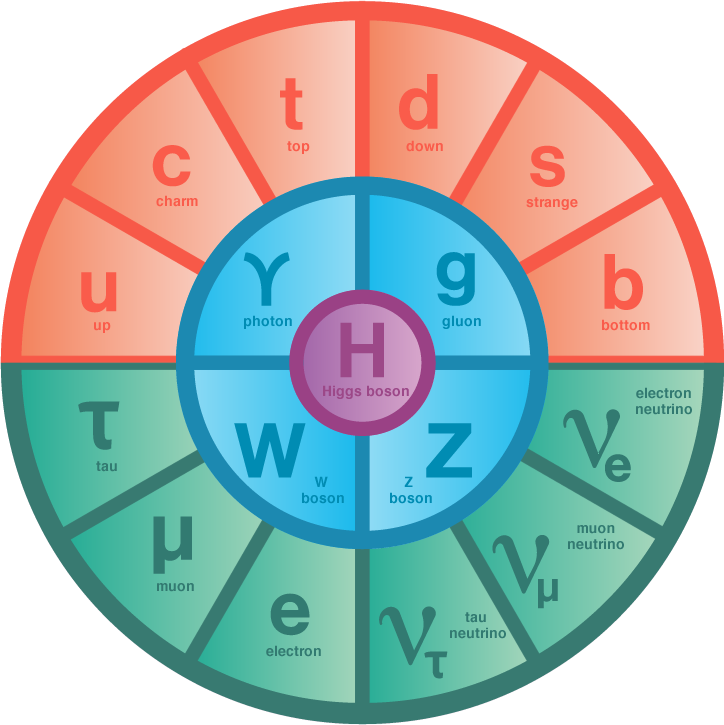
\includegraphics[width=4.2cm, height=4cm]{figs/standard_model.png}
	}
   \end{minipage} \hfill \vfill
     
     	%\begin{itemize}
	\justifying
	%\item 
	\begin{block}{}
	\justifying
	\vspace{5pt}
	$\rightarrow$ However, this model is known to have \textbf{several shortcomings} which require further investigation. For example, eventual exotic particles which do not fit within this model (such as dark matter) are extensively searched for nowadays. \vspace{5pt}
	\end{block} \vfill
	%\end{itemize}
	
\end{frame}


\begin{frame}{Dark matter}
	
   \begin{minipage}[c]{.49\linewidth}
   	%\begin{itemize}
	\justifying
	%\item 
	The dark matter hypothesis was introduced as a way to explain the strange behavior of the \textbf{rotation curves} of the galaxies at high radius, and the apparent \textbf{missing mass} in the Universe. \vfill
	%\end{itemize}
   \end{minipage} \hfill
   \begin{minipage}[c]{.49\linewidth}
   	\centering{
		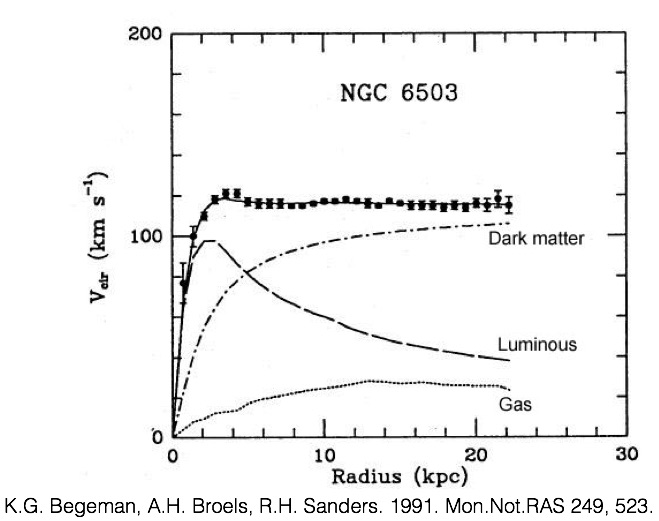
\includegraphics[width=4cm, height=2.5cm]{figs/RotationCurve2.jpeg}
	}
   \end{minipage} \hfill \vfill	
   
   \begin{minipage}[c]{.34\linewidth}
   	\centering{
		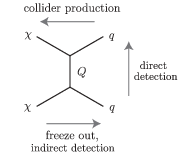
\includegraphics[width=3cm, height=2.2cm]{figs/detection.png}
	}
   \end{minipage} \hfill
   \begin{minipage}[c]{.64\linewidth}
   %\begin{itemize}
   	\justifying
	%\item 
	Ordinary baryonic matter constitutes only  5\% of the total mass of the Universe, while the dark matter accounts for 27\%. \vfill \vspace{8pt}We also assume that dark matter is \textbf{made out of cold particles} and interact only weakly with ordinary matter or itself, making it \textbf{extremely difficult to detect}.
	%\end{itemize}
    \end{minipage} \hfill \vfill	
    
    \begin{block}{}
	\justifying
	\vspace{5pt}
   $\rightarrow$ Since we do not know any baryonic candidate fulfilling these conditions, we can postulate the \textbf{existence of new elementary particles}, the WIMPs. This is typically the kind of particles we \textbf{hope to find at the LHC}. \vspace{5pt}
    \end{block} \vfill
	
\end{frame}

\begin{frame}{Our channel of interest}

	\justifying
	This work will be focused on \textbf{dark matter production in association with a top and an anti-top quarks}, in the dilepton final state. The dark matter $\chi$ is produced through the interaction of two gluons and through the apparition of a \textbf{mediator $\Phi$} for which we will consider \textbf{different masses and couplings} (scalar and pseudoscalar). \\ \vspace{8pt} \vfill
	
	\begin{minipage}[c]{.39\linewidth}
	\centering{
		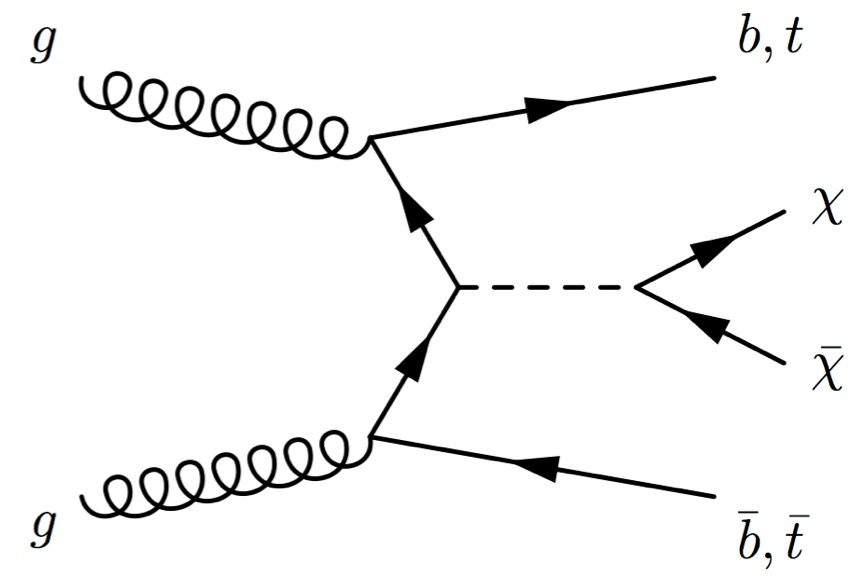
\includegraphics[width=3.2cm, height=2.5cm]{figs/feynman2.jpg}
	}
   	\end{minipage} \hfill
   	\begin{minipage}[c]{.59\linewidth}
	\justifying
	\color{mycolor} We are looking at this channel mainly because... \color{black} 
	\begin{itemize}
	\justifying
	\item The \textbf{signature left by the top quarks} can be isolated well with respect to the other backgrounds' leftovers. \vfill
	\item If we assume that the dark matter mediator couples in the same way than the Higgs does, it should have \textbf{stronger couplings with heavier particles} (and the top is the most massive fermion known). \vfill
	\end{itemize}
   	\end{minipage} \hfill \vfill	
	
	\vspace{8pt}
	
	The dilepton final state is interesting because, even though this is the channel with the \textbf{smallest branching ratio} (fraction of times for which a particle decays by an individual decay mode with respect to the total number of decays), this is also the channel having the \textbf{least number of backgrounds}. \vfill

\end{frame}


\begin{frame}{The Large Hardon Collider}

	\begin{minipage}[c]{.49\linewidth}
	\centering{
		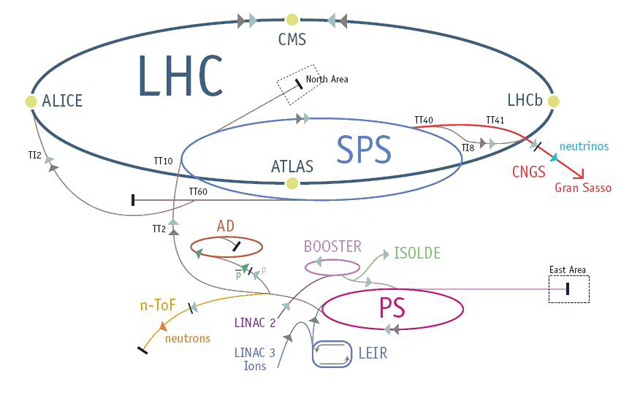
\includegraphics[width=4.2cm, height=3.1cm]{figs/lhc2.jpg}
	}
   	\end{minipage} \hfill
   	\begin{minipage}[c]{.49\linewidth}
	\justifying
	The data has been taken by the Large Hardron Collider, a \textbf{circular underground proton-proton collider}, situated at CERN. With its 27 kilometers of circumference, it is currently the \textbf{most powerful accelerator} in the world. \\ \vspace{10pt}
	It is the result of a collaboration of 22 countries, and has been built in order to study and reproduce the Universe at its origin. \vfill
   	\end{minipage} \hfill \vfill	

	\begin{block}{\vspace{5pt} The LHC in a nutshell}
	\begin{itemize}
	\justifying
	\vspace{5pt}
	\item Beams of protons circulate in opposite directions at velocities close to the speed of light and collide in 4 different points, where the detectors are. \\ \vspace{3pt}
	\item Accelerates 2808 bunches of 10$^{11}$ protons up to a center of mass energy of 13 TeV so far (but has been designed to reach 14 TeV). \\ \vspace{3pt}
	\item Can reach an instantaneous luminosity of 10$^{34}$ cm$^{-2}$s$^{-1}$ and a collision rate of 40 MHz.\\ \vspace{5pt}
	\end{itemize}
	\end{block} \vfill
	
\end{frame}

\begin{frame}{The Compact Muon Solenoid}
	\begin{minipage}[c]{.49\linewidth}
	\justifying
	CMS is one of the two \textbf{polyvalent detectors} of the LHC, designed to make measurements in most of the major different fields of particle physics, from precision measurements to the search of new exotic processes. \\ \vspace{10pt}
	\centering{
		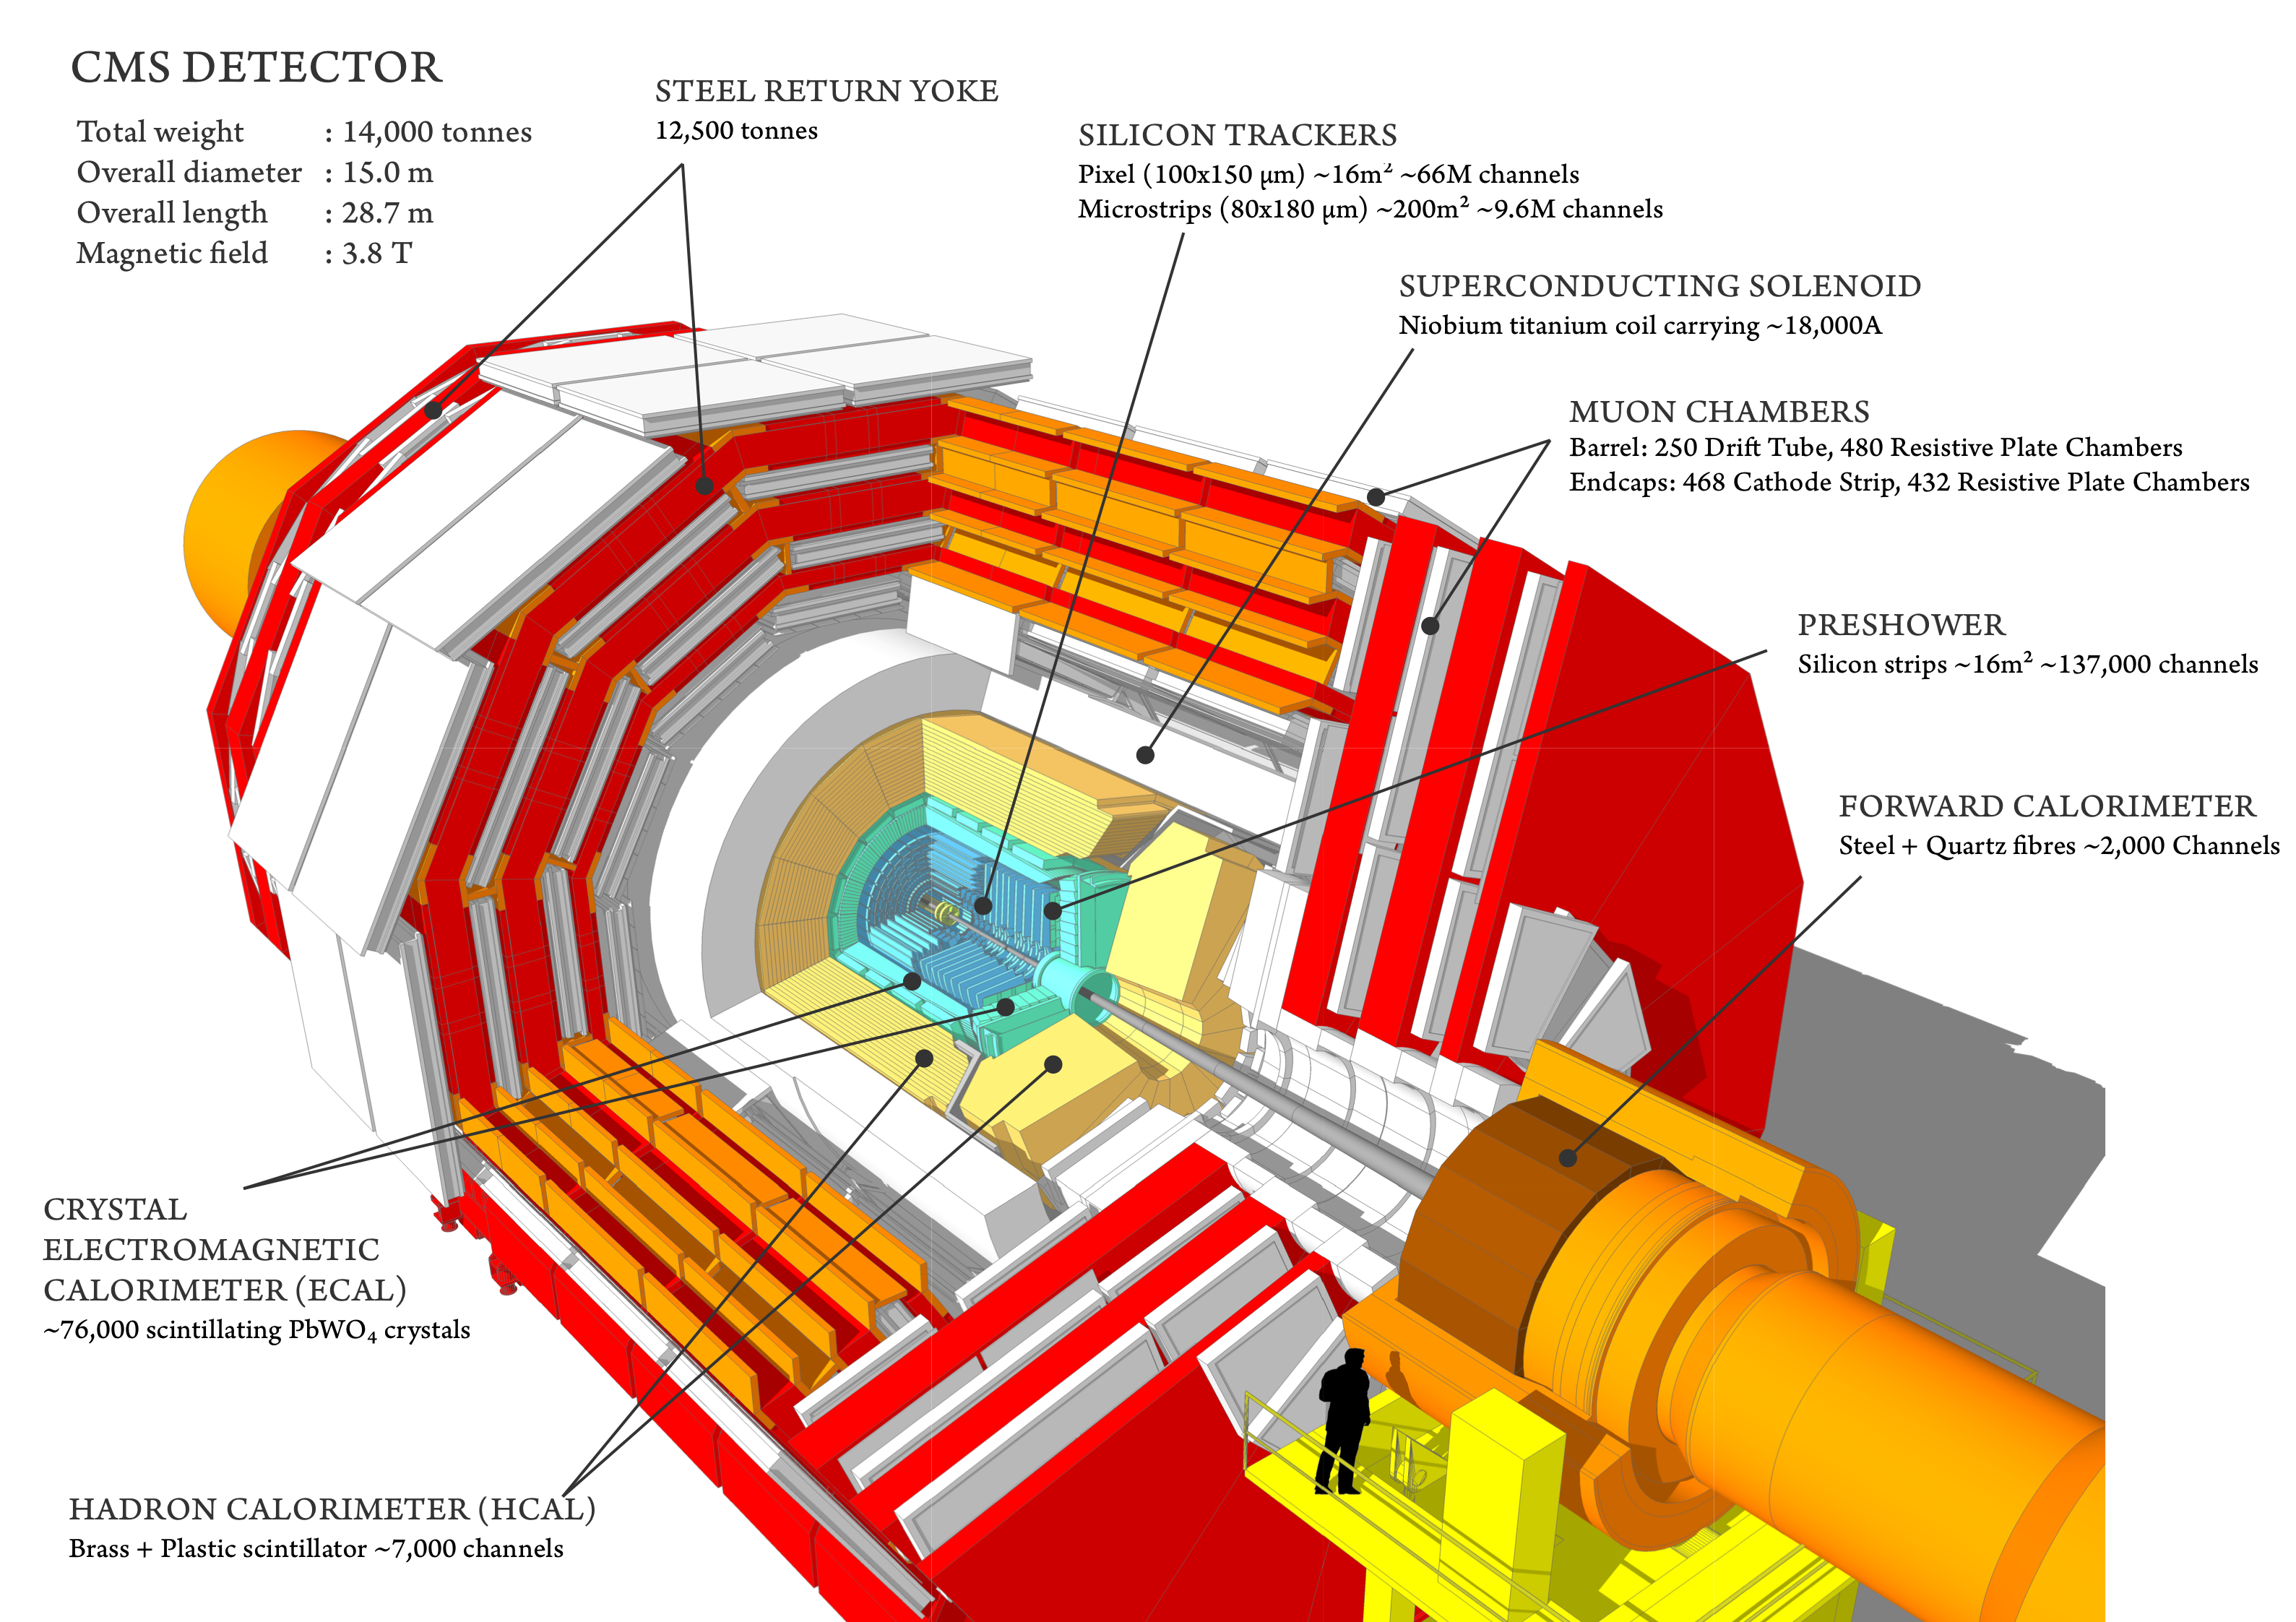
\includegraphics[width=6.2cm, height=4.9cm]{figs/CMS.png} 
	} \vfill
   	\end{minipage} \hfill
   	\begin{minipage}[c]{.42\linewidth}
		\begin{block}{\vspace{5pt} CMS in a nutshell}
	\begin{itemize}
	\justifying
	\vspace{5pt}
	\item Is a \textbf{compact} detector (its 14.000 tons are compacted in a relatively small volume). \\ \vspace{3pt}
	\item Has a \textbf{powerful tracker and muon detection system} allowing us to measure some of the properties of the leptons throughout a large range of energies. \\ \vspace{3pt}
	\item Has a \textbf{huge solenoid} as central piece able to produce a 3.8T magnetic field, to curve the particles and study their properties. \\ \vspace{3pt}
	\item Is made out of \textbf{different layers} (such as the tracker, the calorimeters and the muon chambers), each having its own purpose. \\ \vspace{5pt}
	\end{itemize}
	\end{block}
   	\end{minipage} \hfill \vfill	
\end{frame}


\begin{frame}{What are we looking for?}

	\justifying
	For an event to be considered interesting, we basically require the presence of exactly \textbf{two energetic leptons}, at least \textbf{two b-jets} and some \textbf{missing transverse energy} (corresponding to the unbalanced transverse momentum of the collision). \vspace{8pt}

	\begin{exampleblock}{} Two leptons and two b-jets \end{exampleblock} \vspace{8pt}

	\begin{minipage}[c]{.59\linewidth}
	\justifying
	We are looking for dark matter produced with a top and an anti-top, which are not stable and decay immediately to a W$^\pm$ and a bottom quark. We are then searching for the results of the \textbf{hadronisation of the bottom} quarks, and for \textbf{two leptons coming from the W$^\pm$}. \vfill
   	\end{minipage} \hfill
   	\begin{minipage}[c]{.39\linewidth}
	\centering{
		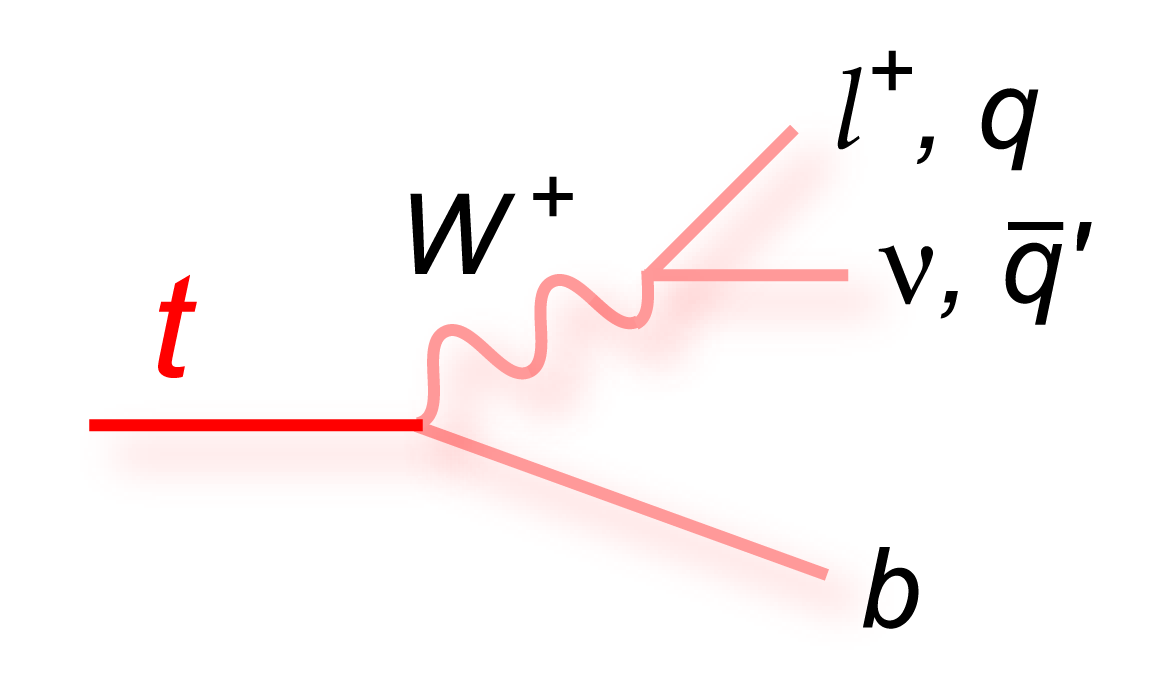
\includegraphics[width=3.2cm, height=2.2cm]{figs/top_decay.png} 
	}
	\end{minipage} \hfill \vfill
	
	\begin{exampleblock}{} Missing transverse energy \end{exampleblock}
	
	\vspace{8pt}
	\justifying
	Moreover, since dark matter particles do not interact with ordinary matter, we do not expect this kind of particles to \textbf{interact at all with the detector}. We are then also looking for a large amount of \textbf{missing transverse energy}. \vfill

\end{frame}


\begin{frame}{Datasets and triggers}

	\begin{exampleblock}{} The datasets... \end{exampleblock}
	
	\vspace{8pt}
	\begin{minipage}[c]{.59\linewidth}
	\begin{itemize}
	\justifying
	\item Have been recorded during 7 different periods and have been selected to match the current \textbf{blinding policy} (we look at the already published 2.4 fb$^{-1}$ for the signal region, and at the full 35.9 fb$^{-1}$ for the control regions). \\ \vspace{8pt}
	\item This blinding policy consists in optimizing the analysis considering a \textbf{limited dataset} only, to avoid any \textbf{conscious or unconscious bias} when one tries to optimize his analysis based on what has already been seen.
	\end{itemize} \vfill
   	\end{minipage} \hfill
   	\begin{minipage}[c]{.39\linewidth}
	\begin{center}
	\resizebox{95pt} {!}{
	\begin{tabular}{c|c}
		& \\
		Era & Luminosity (fb$^{-1}$) \\
		& \\
		\hline \hline
		& \\
		Run2016B & 5.748 \\
		Run2016C & 2.573 \\
		Run2016D & 4.248 \\
		Run2016E & 4.009 \\
		Run2016F & 3.102 \\
		Run2016G & 7.540 \\
		Run2016H & 8.606 \\ 
		& \\ 
		\hline
		& \\
		Total & 35.827 \\
		& \\
	\end{tabular}
	}
	\end{center}
   	\end{minipage} \hfill \vfill	
	
	\begin{exampleblock}{} The triggers... \end{exampleblock}
	\begin{itemize}
	\justifying
	\item Are used to \textbf{store only interesting events} out of the 40 MHz of collisions produced. \\ \vspace{8pt}
	\item Have been chosen and combined to only select events with at least 1 or 2 leptons while trying to maximize the efficiency of selection.
	\end{itemize} \vfill 
	
\end{frame}


\begin{frame}{Background processes}

	\justifying
	Different backgrounds have similar final state, distributions and/or signatures than the ones expected for our signal. Here are the most important ones. \vfill
	
	\begin{itemize}
	\justifying
	\item $t \bar t$ $\rightarrow$ is our main background and has kinematics close to the expected ones for our signal. The biggest challenge of the analysis consists in finding ways to reduce this background while leaving the signal as it is. \vspace{8pt} 
	
\begin{minipage}[c]{.24\linewidth}
   	\centering{
		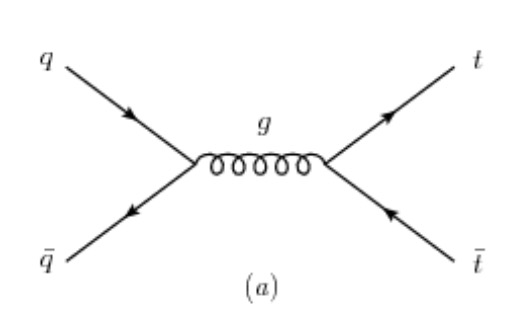
\includegraphics[width= 60pt, height= 45pt]{figs/tt1.jpg} \\
	}
   \end{minipage}
   \begin{minipage}[c]{.24\linewidth}
   	\centering{
		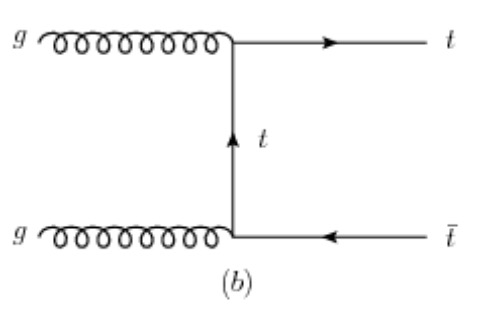
\includegraphics[width= 60pt, height= 45pt]{figs/tt2.jpg} \\
	}
\end{minipage}
	 \begin{minipage}[c]{.24\linewidth}
   	\centering{
		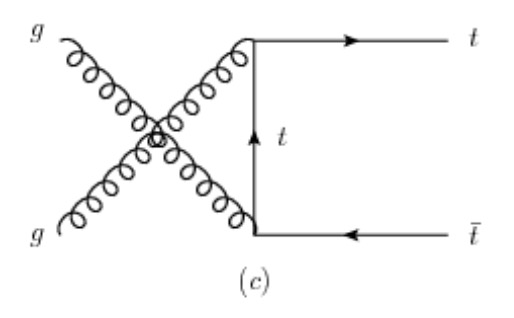
\includegraphics[width= 60pt, height= 45pt]{figs/tt3.jpg} \\
	}
\end{minipage}
	\begin{minipage}[c]{.24\linewidth}
   	\centering{
		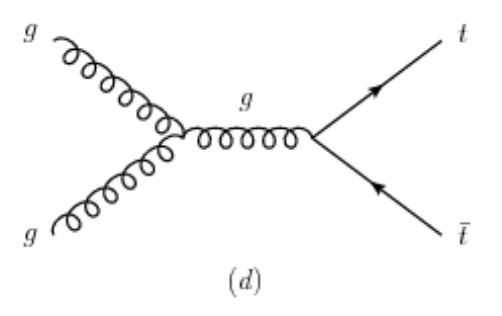
\includegraphics[width= 60pt, height= 45pt]{figs/tt4.jpg} \\
	}
\end{minipage} \vspace{8pt} 
	
	\item $t W^\pm$ $\rightarrow$ having a lower cross section and different kinematics, this background has a lower impact on the final results, even though it features a two b-jets and missing transverse energy in the final state as well. \\ \vspace{8pt} 
	%\item Non-prompt $\rightarrow$ appears basically when a jet is misidentified as a lepton. The impact on the final yields has been calculated by applying a general tight-to-loose data-driven method. \\ \vspace{8pt} 
	\item ttV (ttW/ttZ) $\rightarrow$ having two top quarks in the final state, some of this process is also expected to survive the selection of the analysis and to have an impact on the final results. \\ \vspace{8pt} 
	\item Other backgrounds $\rightarrow$ such as the Drell-Yan ($Z/\gamma*$) or the non-prompt background also have different kinematics and only a limited impact on the final results. 
	\end{itemize} \vfill
	
\end{frame}


\begin{frame}{Monte Carlo samples}
	
	\begin{itemize}
	\justifying
	\item The different backgrounds have either been simulated with \textbf{Monte Carlo simulations} and checked in \textbf{control regions} (regions enriched in a single background) or measured using \textbf{data-driven methods} (estimated directly from the data). \\ \vspace{8pt} 
	\item The dark matter samples have also been generated using Monte Carlo simulations. Different samples have been produced, for different \textbf{dark matter mediator masses} (10, 20, 50, 100, 200, 300 and 500 GeV), considering both the \textbf{scalar and pseudoscalar mediator couplings}.
	\end{itemize} \vfill 

\hspace{4pt}
\begin{minipage}[c]{.02\linewidth}
	\begin{exampleblock}{} \rotatebox{90}{ MC samples used } \end{exampleblock}
\end{minipage}	
\hspace{8pt}
\begin{minipage}[c]{.28\linewidth}
\begin{table}
\centering
\resizebox{95pt} {!}{
\begin{tabular}{c|c}
& \\
Background & $\sigma$ [pb] \\
& \\
 \hline \hline
 & \\
$t \bar t \rightarrow$ ll $\nu$$\nu$ & 87.31 \\
Single top & 35.6  \\
Single antitop & 35.6 \\
$t \bar t$W $\rightarrow$ l $\nu$ & 0.2043  \\
$t \bar t$W $\rightarrow$ $q \bar q$ & 0.4062 \\
$t \bar t$Z $\rightarrow$ ll $\nu$$\nu$ & 0.2529 \\
$t \bar t$Z $\rightarrow$ $q \bar q$ & 0.5297  \\
Z $\rightarrow$ ll (low $m_{ll}$) & 18610  \\
Z $\rightarrow$ ll (high $m_{ll}$) & 6025.2  \\
W$\gamma \rightarrow$ l $\nu$ $\gamma$ & 586 \\
Z$\gamma \rightarrow$ ll $\gamma$ & 131.3 \\
& \\
\end{tabular}
}
\end{table} 
   	\end{minipage} \hfill
   	\begin{minipage}[c]{.22\linewidth}
	\begin{center}
	\begin{exampleblock}{} \begin{center} Scalar \\ mediators \end{center} \end{exampleblock}
	\end{center}
	\vspace{-8pt}
\begin{table}
\centering
\resizebox{74pt} {!}{
\begin{tabular}{c|c}
& \\
$m_S$ [GeV] & $\sigma$ [pb] \\
& \\
 \hline \hline
 & \\
10 & 19.950 \\
20 & 10.480 \\
50 & 2.941 \\
100 & 0.672 \\
200 & 0.093 \\
300 & 0.029 \\
500 & 0.005 \\
& \\
\end{tabular}
}
\end{table} 	
   	\end{minipage} \hfill
	\begin{minipage}[c]{.22\linewidth}
	\begin{center}
	\begin{exampleblock}{} \begin{center} Pseudoscalar mediators \end{center} \end{exampleblock}
	\end{center}
	\vspace{-8pt}
\begin{table}
\centering
\resizebox{74pt} {!}{
\begin{tabular}{c|c}
& \\
$m_P$ [GeV] & $\sigma$ [pb] \\
& \\
 \hline \hline
 & \\
10 & 0.441 \\
20 & 0.399 \\
50 & 0.303 \\
100 & 0.191 \\
200 & 0.084 \\
300 & 0.040 \\
500 & 0.005 \\
& \\
\end{tabular}
}
\end{table} 	
   	\end{minipage} \hfill \vfill	
	
\end{frame}


\begin{frame}{Event reconstruction}

	\begin{block}{\vspace{5pt} Reconstruction of the objects}
	\justifying
	\vspace{5pt}
	A particular algorithm, the Particle Flow, is usually used in order to \textbf{gather the information} coming from the different parts of the detector and to \textbf{reconstruct the tracks} of the different particles.\vspace{5pt}\vfill
	\end{block}

	\vspace{8pt}

	\begin{minipage}[c]{.54\linewidth}
   	\centering{
		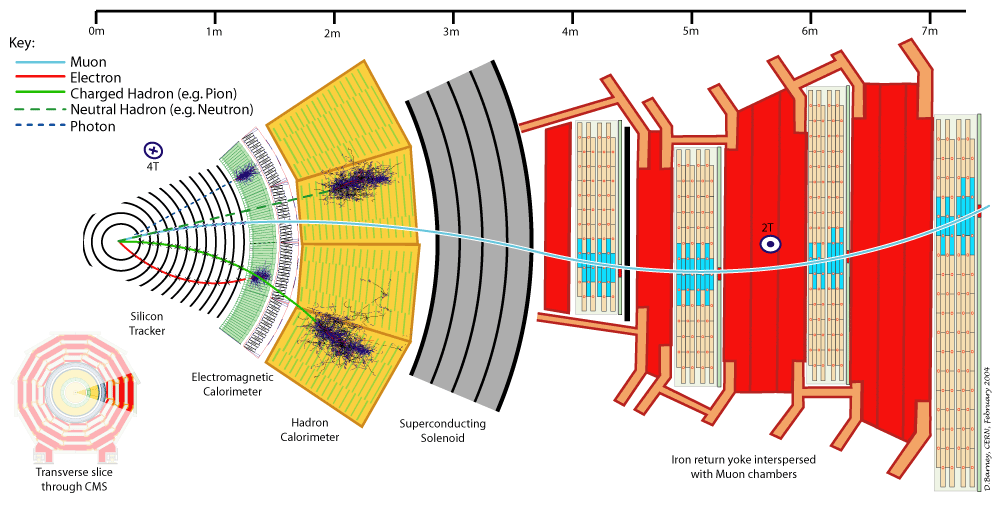
\includegraphics[width=5.4cm, height=3.6cm]{figs/CMS_inside.png} \vfill
	}
	\end{minipage}
	 \begin{minipage}[c]{.44\linewidth}
   		\justifying 
		The geometry of the detector is quite simple. Usually, the z-axis is defined as the axis followed by the beams, meaning that the $O_{xy}$ plane (also called $\Phi$ plane) corresponds to the transverse plane of the detector. \\ \vspace{8pt}
		The pseudorapidity $\eta$ is a Lorentz invariant quantity defined as $-ln\left(tan(\frac{\theta}{2}) \right)$ where $\theta$ is the angle between the z- and x-axes.
		
	\end{minipage}
	
	\vspace{5pt}
	\justifying
	In this analysis, only \textbf{isolated tight leptons} (complying with a lot of different requirements, resulting in better leptons) having a $p_T$ larger than 10 GeV and $|\eta|$ smaller than 2.5 (2.4) for electrons (muons) are considered. Jets are required have a $p_T$ larger than 30 GeV and $|\eta|$ smaller than 4. \vfill

\end{frame}


\begin{frame}{Top reconstruction}

	\begin{block}{\vspace{5pt} General idea}
	\justifying
	\vspace{5pt}
	The top reconstruction is a general method developed to calculate the $p_T$ of the tops in any $t \bar t$-like event. We extended this method so that it is also \textbf{able to measure the $p_T$ of the mediator} produced in the dark matter case.\\ \vspace{8pt}
	\end{block} \vfill
	
	\justifying
	Having a way to determine the $p_T$ of the mediator is interesting, because this variable is expected to \textbf{give us a good discrimination} between the $t \bar t$ and our signal. \vfill
	
   \begin{minipage}[c]{.24\linewidth}
   	\centering{
		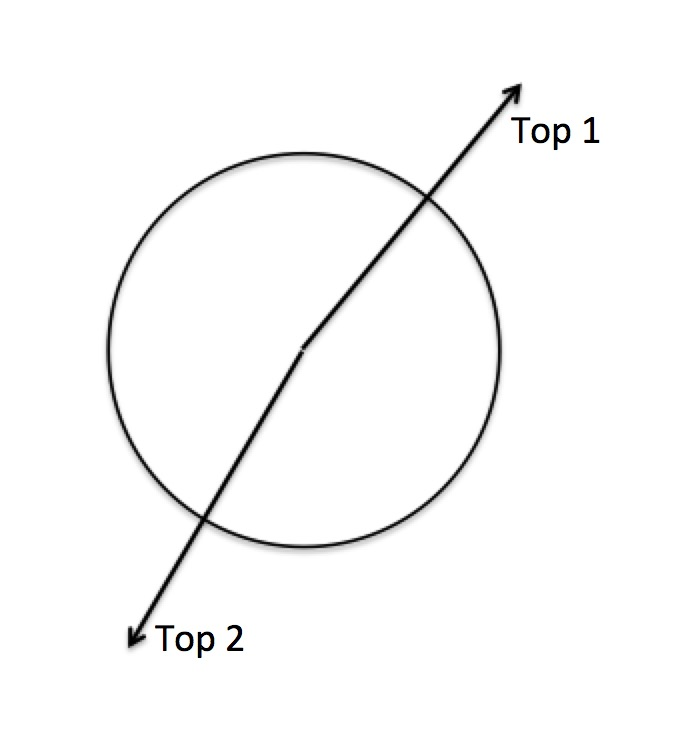
\includegraphics[width= 80pt, height= 80pt]{figs/tt.jpg}
	}
   \end{minipage} \hfill
   \begin{minipage}[c]{.24\linewidth}
   	\justifying
	In the usual $t \bar t$, both the tops are expected to leave the primary vertex back-to-back.
   \end{minipage} \hfill
   \begin{minipage}[c]{.24\linewidth}
   	\centering{
		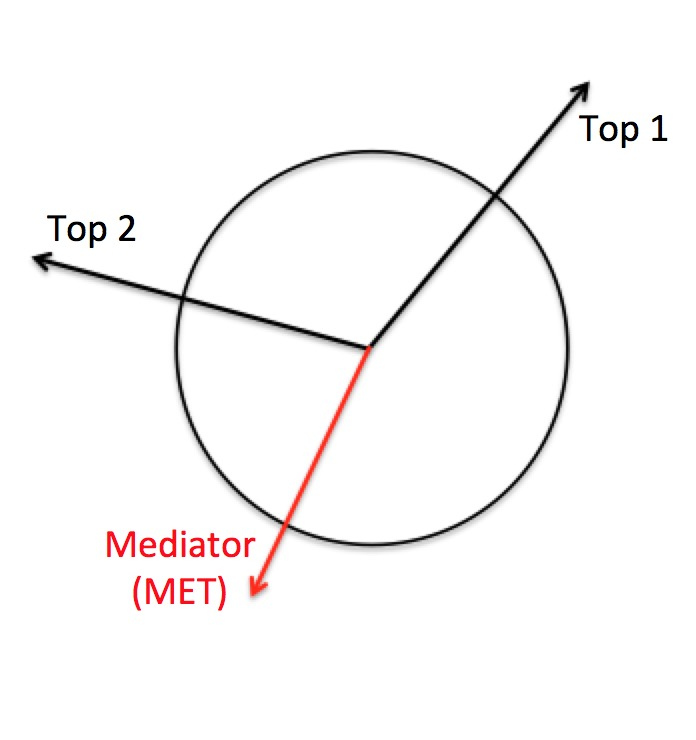
\includegraphics[width= 80pt, height= 80pt]{figs/ttandDM.jpg}
	}
   \end{minipage} \hfill
   \begin{minipage}[c]{.24\linewidth}
   	\justifying
	In the $t \bar t$ + DM case, the mediator leaves the primary vertex with a $p_T$ equal to the difference in $p_T$ of the tops.
   \end{minipage} \hfill \vfill

	\justifying
	An event passing the usual top reconstruction gets a value of dark $p_T$ exactly equal to 0, while an event passing moreover our improved reconstruction (and therefore more likely to be a signal event) gets a value higher than 0. \vfill

\end{frame}


\begin{frame}{Event preselection}

	\justifying
	We want to be able to reduce as much as we possible can the background, while keeping as much signal as possible by applying several cuts on different variables. This is first done by cutting in several general variables. \vfill  %(the values where to cut have been determined in order to optimize the significance of the signal). \vfill 

\hspace{4pt}
   \begin{minipage}[c]{.02\linewidth}
	\begin{exampleblock}{} \rotatebox{90}{ Preselection of the analysis } \end{exampleblock}
   \end{minipage}	
   \hspace{2pt}
   \begin{minipage}[c]{.97\linewidth}
   \begin{center}
   \resizebox{300pt} {!}{
   \begin{tabular}{c|c|c|c}
   Number & Cut level & Cut & Comment \\
   	& & & \\
   	\hline \hline
	& & & \\
	  \multirow{4}{*}{0} & \multirow{4}{*}{Preselection} & $p_{T}^{lep_1} >$ 25 GeV & On the leading lepton\\ 
	  & & $p_{T}^{lep_2}$ $>$ 20 GeV & On the trailing lepton \\ 
	  & & $p_{T}^{lep_3}$ $<$ 10 GeV &Third lepton veto \\ 
	  & & $q_{l}^{lep_1} \cdot q_{l}^{lep_2} < 0$ & Opposite charge requirement \\ 
	  & & & \\
	  \hline
	   & & & \\
	  \multirow{4}{*}{1} & \multirow{4}{*}{First level} & $m_{ll} > 20$ GeV &  \\
	  & & $|m_{ll} - m_Z| > 15$ GeV & Only applied to $ee$ and $\mu \mu$ channels \\
	  & & $n_{jet} \geq 2$ &  \\
	  & & $n_{b_{jet}} \geq 1$ &  \\
	  & & & \\
   \end{tabular}
   } 
   \end{center}
   \end{minipage} \hfill \vfill

	\justifying
	All these cuts allow us to reduce strongly different backgrounds (such as the Drell-Yan). However, we still need to find other variables able to remove some of the $t \bar t$, the most problematic background. \vfill

\end{frame}


\begin{frame}{Discriminating variables}

	\justifying
	In the following plots have been represented the distributions of the number of event for four different variables. These plots have been obtained by applying the cuts corresponding to the preselection of the analysis, and both the 10 (red line) and 500 GeV (brown line) scalar signals have been represented (and \textbf{rescaled} by a factor 10 and 1000, respectively). \vfill
	
	\begin{minipage}[c]{.48\linewidth}
	
   	\begin{center}
	\begin{exampleblock}{} { \begin{center} \vspace{1pt} Dark $p_T$ \vspace{1pt} \end{center}} \end{exampleblock} \vspace{5pt}
	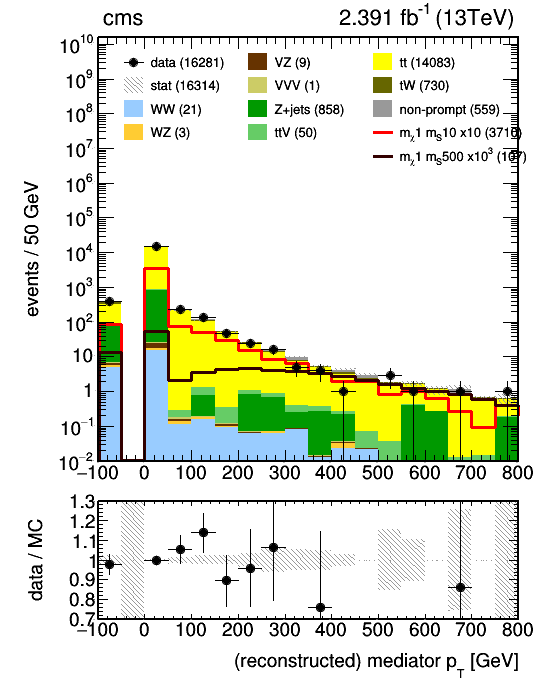
\includegraphics[width= 130pt, height= 115pt]{figs/darkpt_log-preSel3.png} \\
	Reconstructed mediator $p_T$, obtained by applying our top reconstruction method
	\end{center}
	
	\end{minipage}
	\hspace{5pt}
	 \begin{minipage}[c]{.48\linewidth}
   	
	\begin{center}
	\begin{exampleblock}{} { \begin{center} $m_{T2}^{ll}$ \end{center}} \end{exampleblock} \vspace{5pt}
	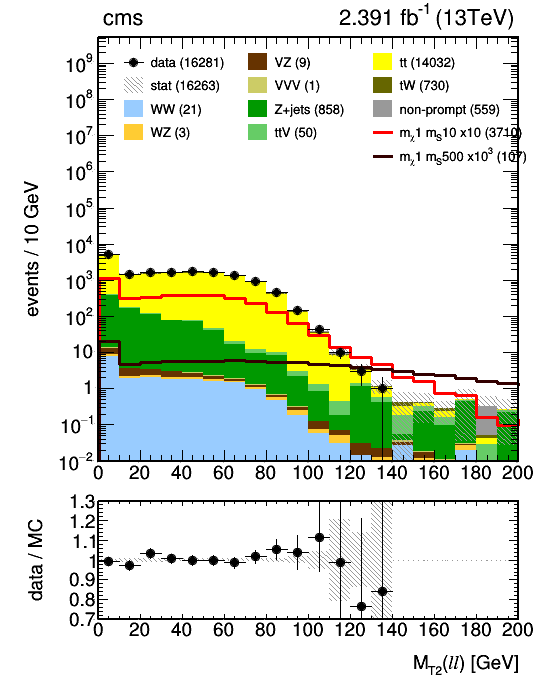
\includegraphics[width= 130pt, height= 115pt]{figs/mt2ll_log-preSel3.png} \\
	Transverse mass of the pair of leptons produced (cf. backup)
	\end{center}
	
	\end{minipage} \vfill

\end{frame}


\begin{frame}{Discriminating variables II}

	\begin{minipage}[c]{.48\linewidth}
	
   	\begin{center}
	\begin{exampleblock}{} { \begin{center} \vspace{0.6pt} $E_T^{\text{miss}}$ \vspace{0.6pt} \end{center}} \end{exampleblock} \vspace{5pt}
	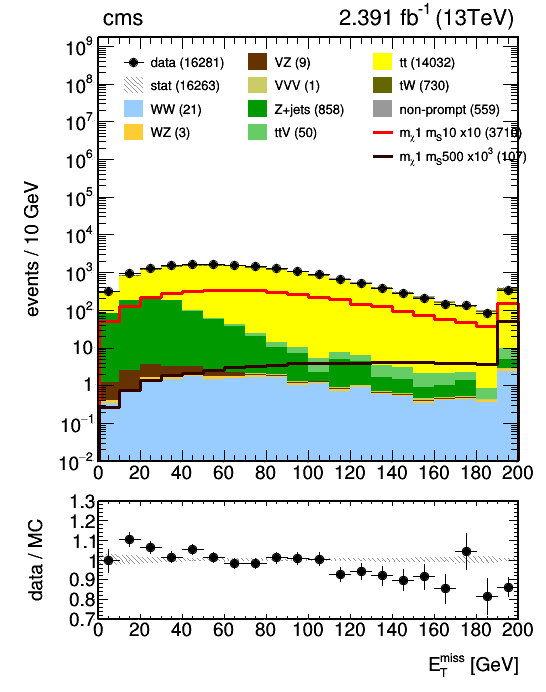
\includegraphics[width= 130pt, height= 115pt]{figs/metPfType1_log-preSel3.png} \\
	Missing transverse energy, equivalent \\ to the imbalance of vector momentum \\ in the O$_{xy}$ plane
	\end{center}
	
	\end{minipage}
	\hspace{5pt}
	 \begin{minipage}[c]{.48\linewidth}
   	
	\begin{center}
	\begin{exampleblock}{} { \begin{center} $\Delta \Phi_{ll, E_T^{\text{miss}}}$ \end{center}} \end{exampleblock} \vspace{5pt}
	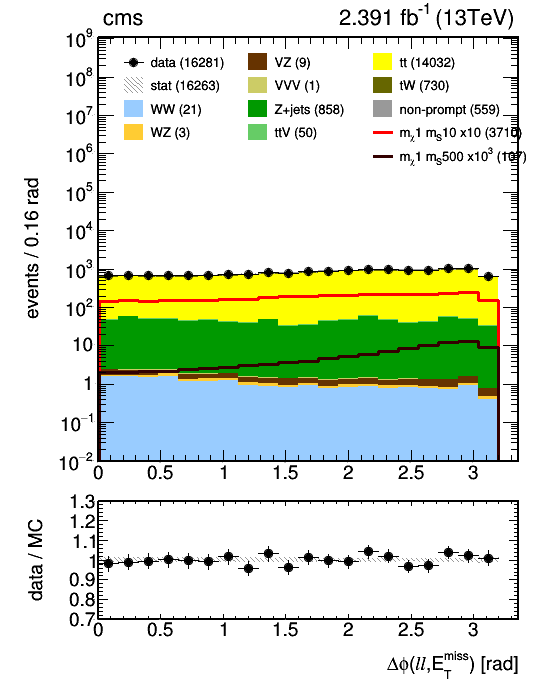
\includegraphics[width= 130pt, height= 115pt]{figs/dphillmet_log-preSel3.png} \\
	Angle between the two leptons coming from the top quarks and \\ the $E_T^{\text{miss}}$ in the O$_{xy}$ plane
	\end{center}
	
	\end{minipage} \vfill

	\begin{block}{}
	\justifying
	Our complete analysis actually lays on the discriminating power of four different variables that will be used as input for our different neural networks, as we will see later. \end{block} \vfill

\end{frame}


\begin{frame}{Final event selection}

	\justifying
	We can then use the previous discriminating variables to introduce a third level of selection, to gain even more in purity. \vfill 

	\hspace{4pt}
   \begin{minipage}[c]{.02\linewidth}
	\begin{exampleblock}{} \rotatebox{90}{ Complete selection of the analysis } \end{exampleblock}
   \end{minipage}	
   \hspace{2pt}
   \begin{minipage}[c]{.97\linewidth}
   \begin{center}
   \resizebox{300pt} {!}{
   \begin{tabular}{c|c|c|c}
   Number & Cut level & Cut & Comment \\
   	& & & \\
   	\hline \hline
	& & & \\
	  \multirow{4}{*}{0} & \multirow{4}{*}{Preselection} & $p_{T}^{lep_1} >$ 25 GeV & On the leading lepton\\ 
	  & & $p_{T}^{lep_2}$ $>$ 20 GeV & On the trailing lepton \\ 
	  & & $p_{T}^{lep_3}$ $<$ 10 GeV &Third lepton veto \\ 
	  & & $q_{l}^{lep_1} \cdot q_{l}^{lep_2} < 0$ & Opposite charge requirement \\ 
	  & & & \\
	  \hline
	   & & & \\
	  \multirow{4}{*}{1} & \multirow{4}{*}{First level} & $m_{ll} > 20$ GeV &  \\
	  & & $|m_{ll} - m_Z| > 15$ GeV & Only applied to $ee$ and $\mu \mu$ channels \\
	  & & $n_{jet} \geq 2$ &  \\
	  & & $n_{b_{jet}} \geq 1$ & \\
	  & & & \\
	  \hline
	  & & & \\
	  \multirow{3}{*}{2} & \multirow{3}{*}{Second level} & $E_T^{\text{miss}}$ $> 80$ GeV &  \\
	  & & $m_{T2}^{ll} >$ 80 GeV &  \\
	  & &  Dark $p_T>$ 0 GeV & Our top reconstruction works \\
	  & & & \\
	  %\hline
	  %& & & \\
	  %3 & Third level & On the ANN output & Will be explained later \\
	  %& & & \\
   \end{tabular}
   } 
   \end{center}
   \end{minipage} \hfill

\end{frame}


%\begin{frame}{Same sign control region}

	%\justifying
	%We also defined a same sign control region in order to study the data-driven method used to calculate the non-prompt background. \vfill

%\end{frame}


\begin{frame}{Multi-Variate Analysis}

	\justifying 
	Performing a general \textbf{cut and count analysis} (applying several cuts on different variables to check for the yields obtained) is not optimal when looking for dark matter, since the \textbf{significance} of the signal is expected to be really low. \\ \vspace{10pt}
	 We then need to come up with solutions to \textbf{extract as much information as we can} from the data. This is why we decided to perform a \textbf{Multi-Variate Analysis}, by using general machine learning techniques and neural networks. \vfill

	\hspace{10pt}
	\begin{minipage}[c]{.45\linewidth}
	
   	\begin{block}{}
	\justifying
	\vspace{5pt}
	The main idea of the MVA consists in using a \textbf{neural network} to combine the information coming from the four previous variables into a single output. \\ \vspace{8pt}
	This should give a way to classify any single event as either background or signal, after training correctly the networks created. \vspace{5pt}
	\end{block}
		
	\end{minipage}
	\hspace{5pt}
	 \begin{minipage}[c]{.48\linewidth}
   	
	\begin{center}
	\vspace{8pt}
	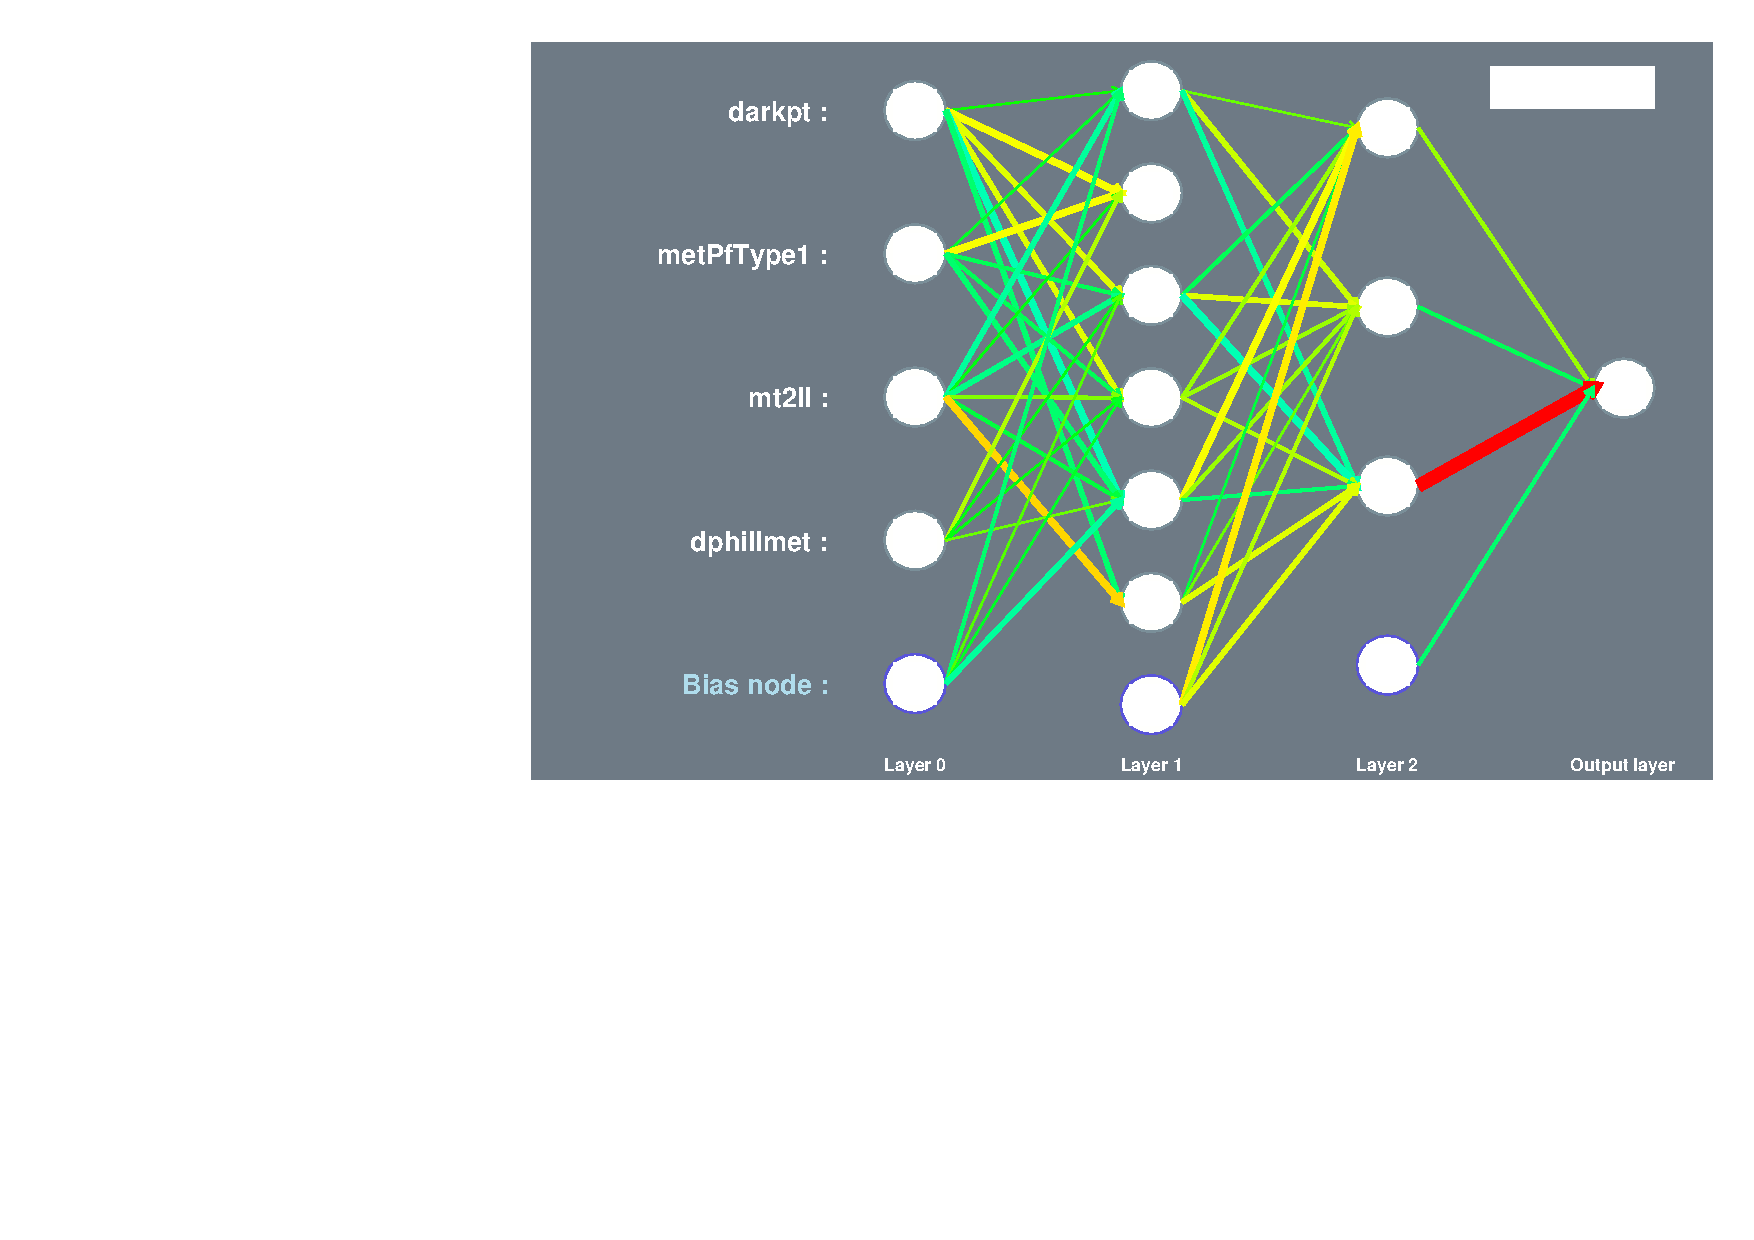
\includegraphics[width=135pt, height=95pt]{figs/newMVA/sigmoid_architecture.pdf}
	\end{center}
	
	\end{minipage} \vfill

\end{frame}


\begin{frame}{Artificial Neural Network}

	\justifying
	Our MVA is performed by defining several different \textbf{neural networks}.
	\begin{itemize}
	\justifying
	\item Each network created contains \textbf{two hidden layers} made out of respectively 6 and 3 neurons. We considered two different kind of neurons, having different \textbf{activation functions}. %(mathematical function applied to get the actual output).
	\item We train a \textbf{different network for each mediator mass} point considered, and for both the scalar and pseudoscalar mediators. The neural networks are trained using 200 events and are trained for the moment only against the $t \bar t$.
	\end{itemize} \vfill

   \hspace{4pt}
   \begin{minipage}[c]{.02\linewidth}
	\begin{exampleblock}{} \rotatebox{90}{ Input distributions } \end{exampleblock}
   \end{minipage}
   \hspace{5pt}
	\begin{minipage}[c]{.44\linewidth}
   	\centering{
		\begin{exampleblock}{}{ \begin{center} 10 GeV scalar mediator \end{center}} \end{exampleblock} \vspace{5pt}
		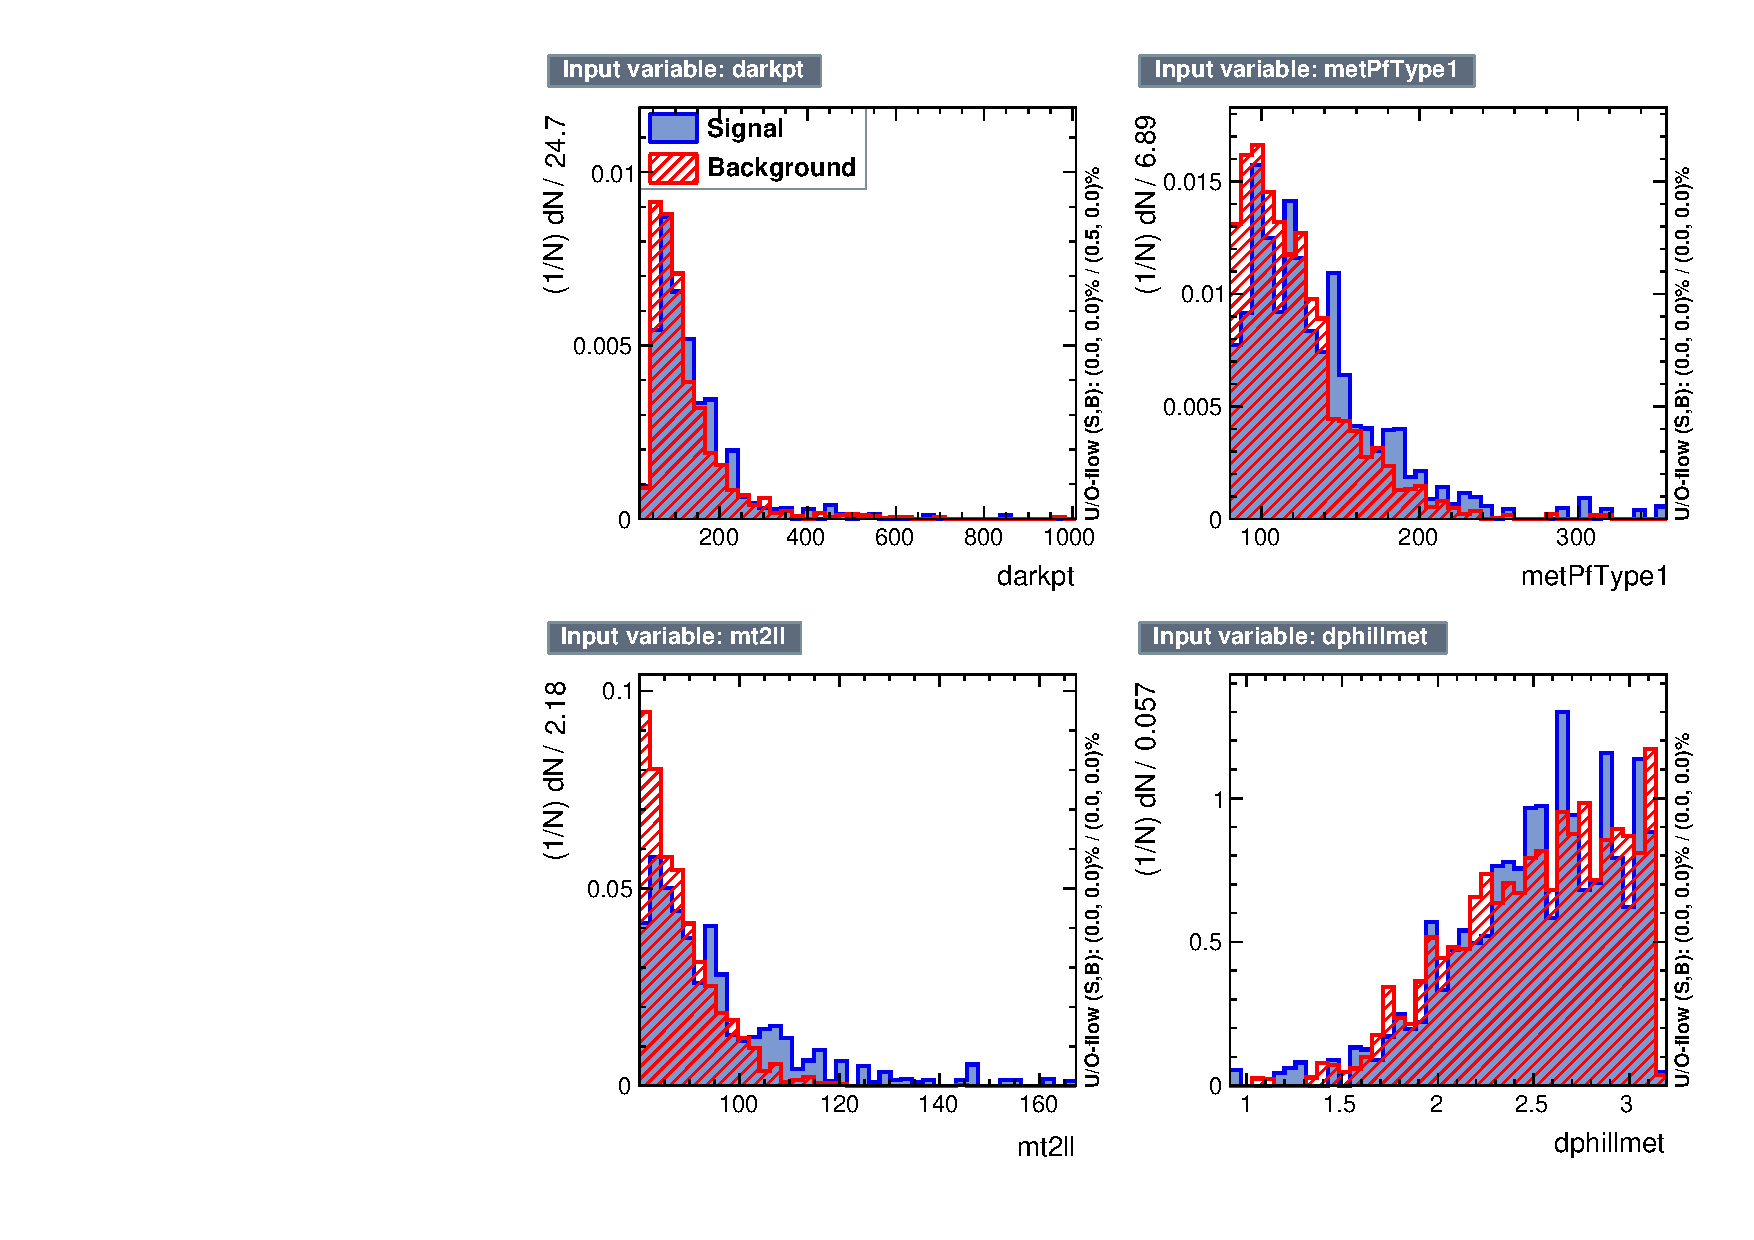
\includegraphics[width=125pt, height=110pt]{figs/newMVA/input_10GeV.pdf}
	}
   \end{minipage} \hfill
   \hspace{10pt}
   \begin{minipage}[c]{.44\linewidth}
   	\centering{
		\begin{exampleblock}{}{ \begin{center} 500 GeV scalar mediator \end{center}} \end{exampleblock} \vspace{5pt}
		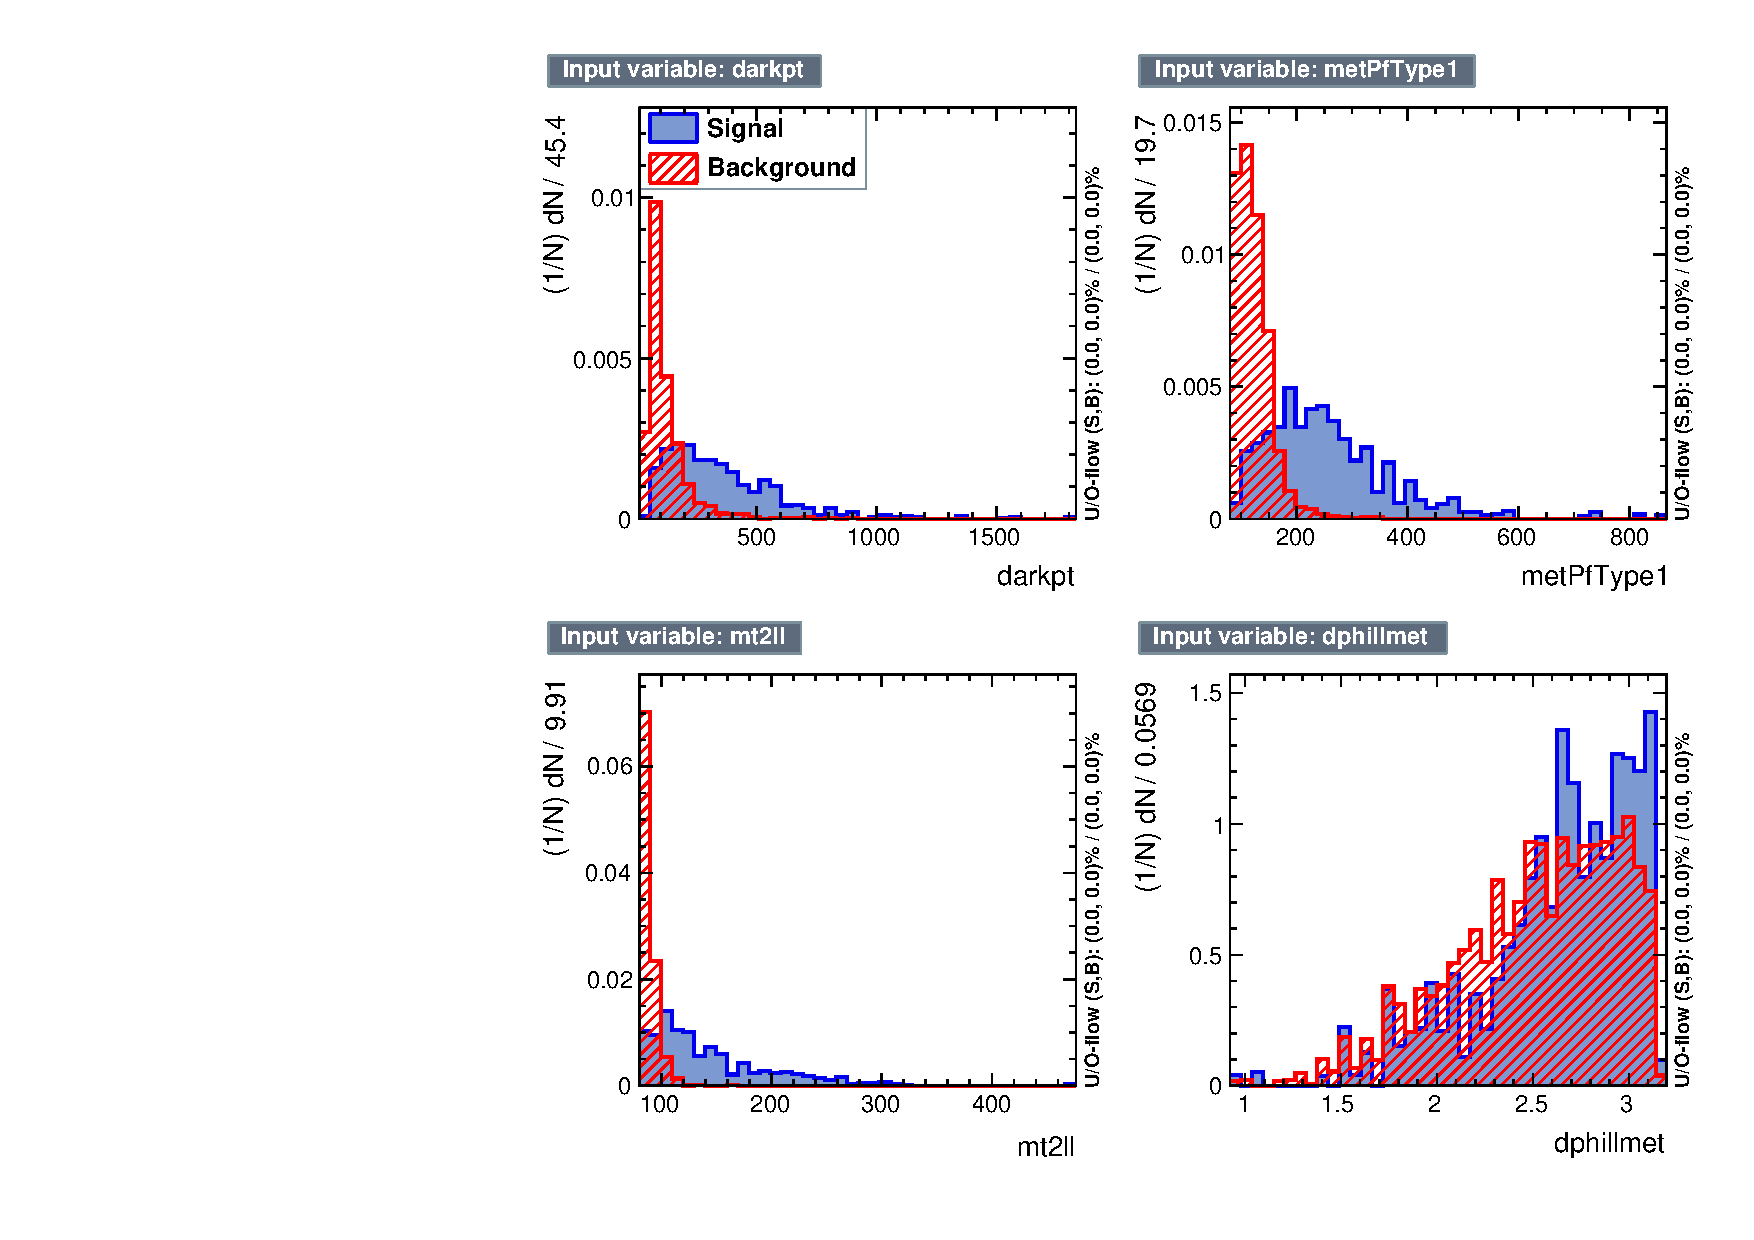
\includegraphics[width= 125pt, height= 110pt]{figs/newMVA/input_500GeV.pdf} \\
	}
   \end{minipage} \hfill \vfill

\end{frame}


\begin{frame}{Artificial Neural Network II}

	\justifying 
	It is also important to check the presence of eventual \textbf{correlations} between the input variables, to make sure not to complicate the networks without valid reason. \vfill

\hspace{4pt}
   \begin{minipage}[c]{.02\linewidth}
	\begin{exampleblock}{} \rotatebox{90}{ $m_\Phi$ = 10 GeV} \end{exampleblock}
   \end{minipage}	
   \hspace{5pt}
   \begin{minipage}[c]{.30\linewidth}
   	\centering{
		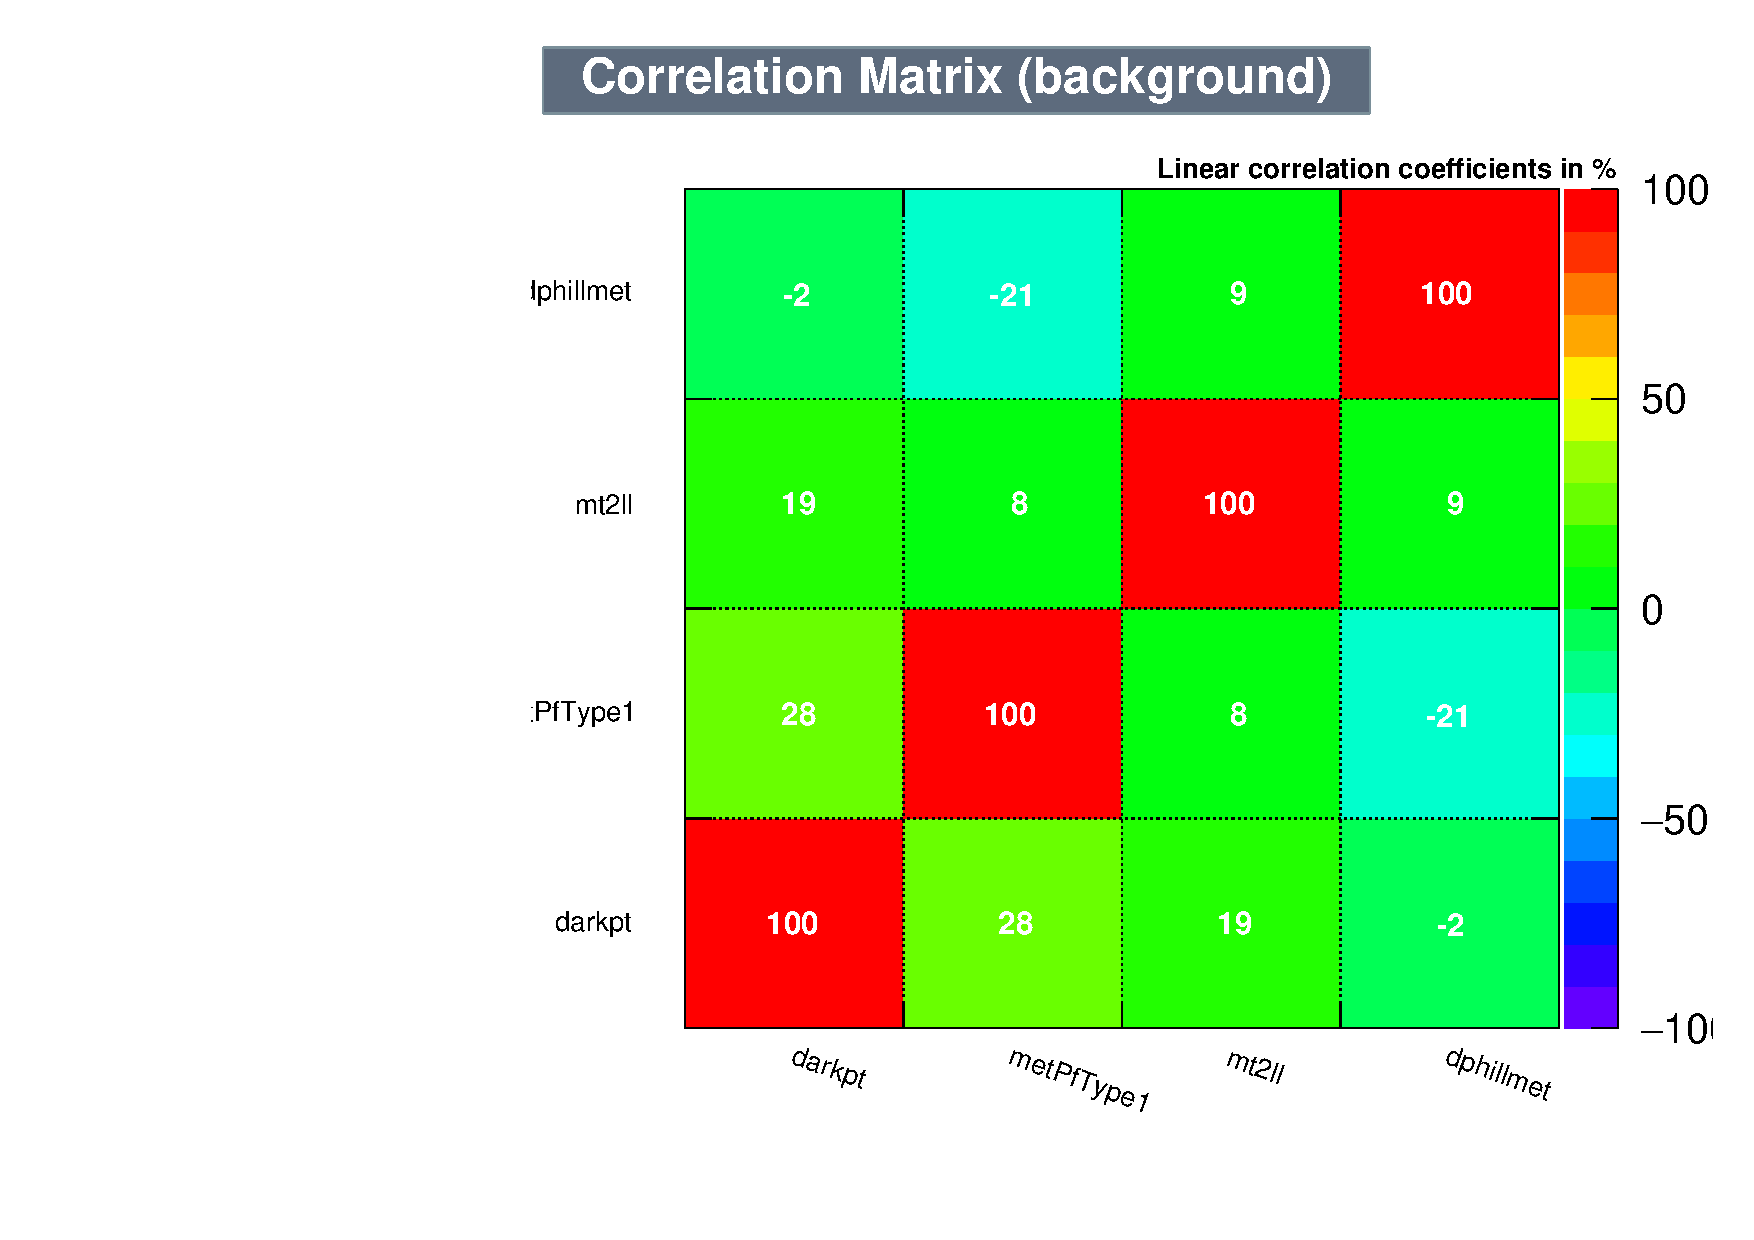
\includegraphics[width= 90pt, height= 90pt]{figs/newMVA/correlation_background_10GeV.pdf}
	}
   \end{minipage} \hfill
   \begin{minipage}[c]{.30\linewidth}
   	\centering{
		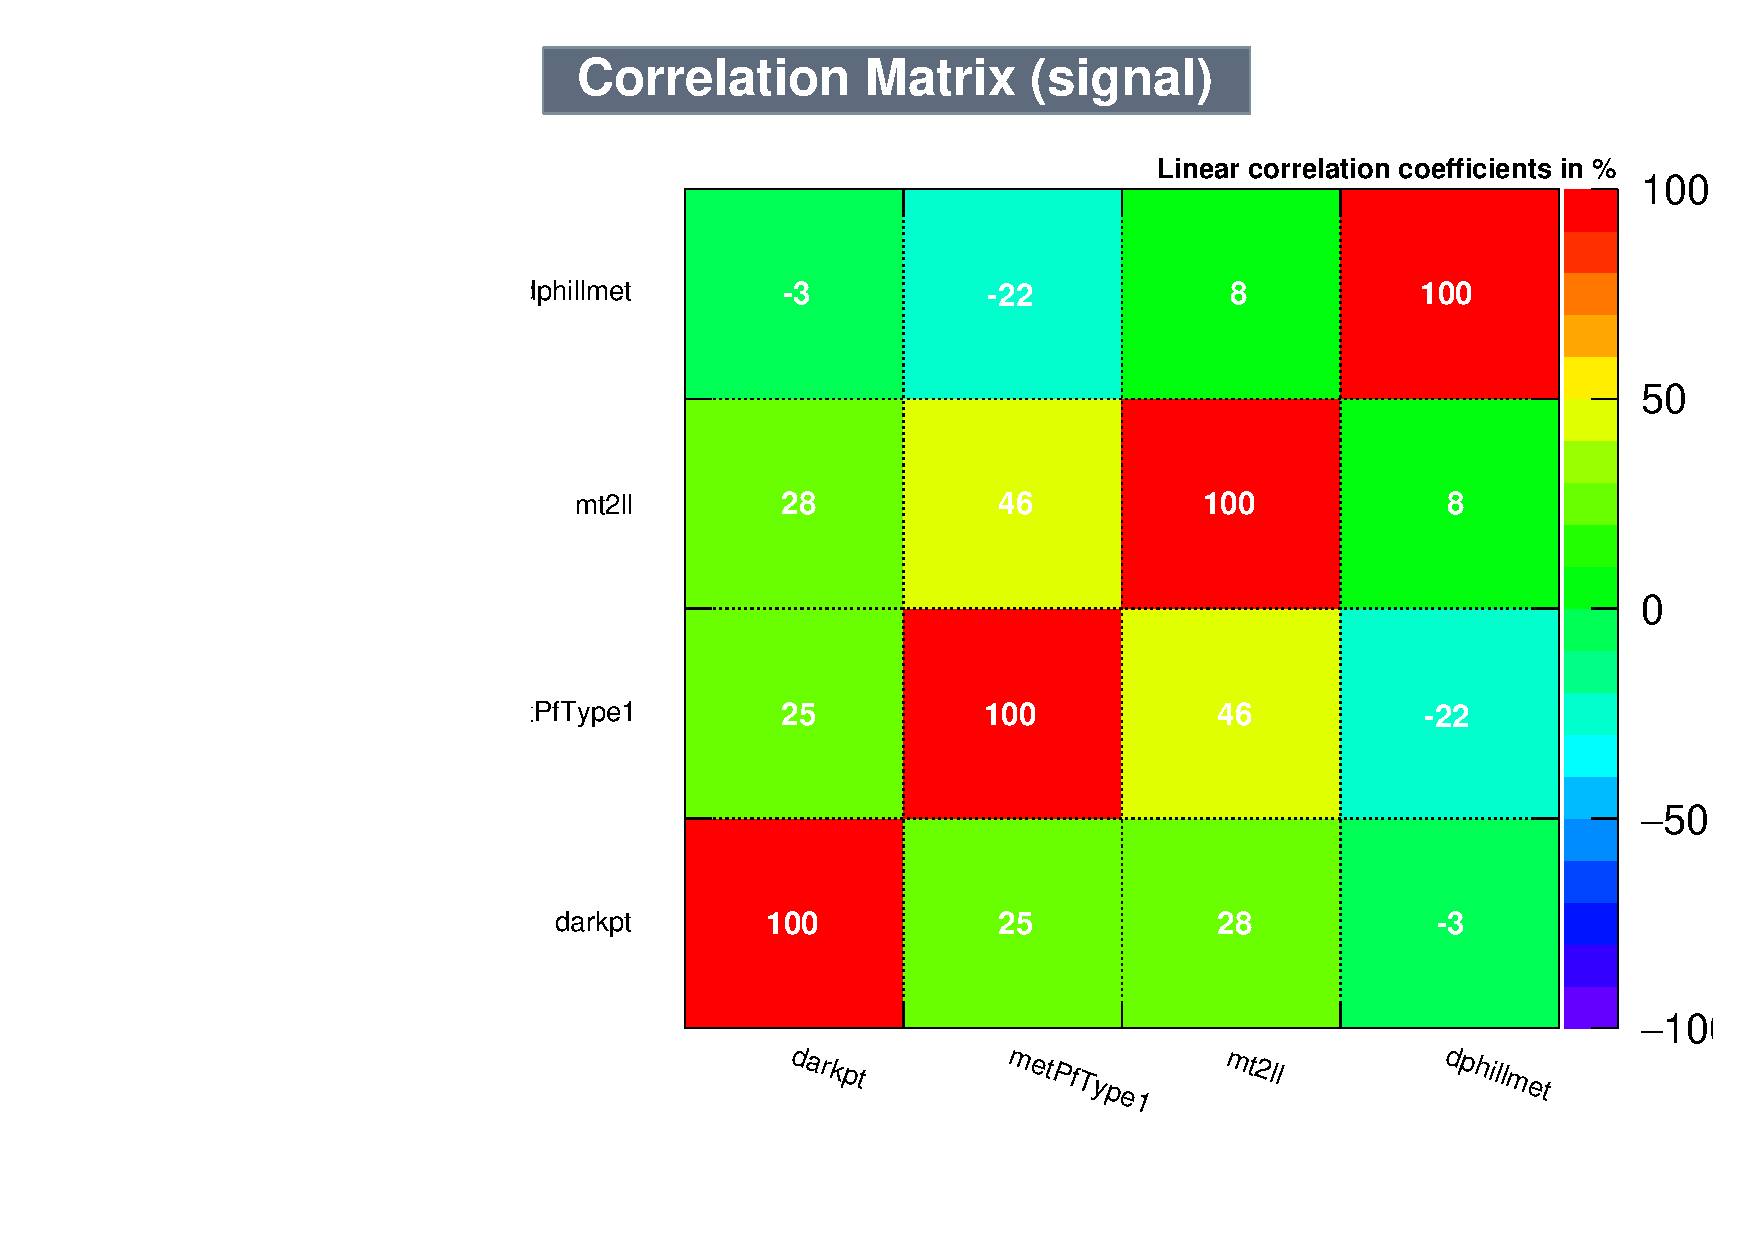
\includegraphics[width= 90pt, height= 90pt]{figs/newMVA/correlation_signal_10GeV.pdf} \\
	}
   \end{minipage} \hfill
   \begin{minipage}[c]{.30\linewidth}
   	\justifying
	The strongest correlation is obtained for the signal, between the $m_{T2}^{ll}$ and the $E_T^{\text{miss}}$ variables (46 \%).
   \end{minipage} \hfill
   %\begin{minipage}[c]{.30\linewidth}
   	%\begin{center} 
	%\resizebox{94pt} {!}{
	%\begin{tabular}{c|c|c}
	%	& & \\
	%	Variable & Sigmoid & Tanh \\
	%	& & \\
	%	\hline \hline
	%	& & \\
	%	dark $p_T$ & 11.06 & 10.93 \\
	%	$m_{T2}^{ll}$ & 7.18 & 3.70 \\
	%	$E_T^{\text{miss}}$ & 3.84 & 4.48 \\
	%	$\Delta \phi_{ll, E_T^{\text{miss}}}$ & 0.58 & 0.82 \\
	%	& & \\
	%\end{tabular}
	%}
	%\end{center}
   %\end{minipage} \hfill
   
  \hspace{4pt}
   \begin{minipage}[c]{.02\linewidth}
	\begin{exampleblock}{} \rotatebox{90}{ $m_\Phi$ =  500 GeV} \end{exampleblock}
   \end{minipage}	
   \hspace{5pt}
   \begin{minipage}[c]{.30\linewidth}
   	\centering{
		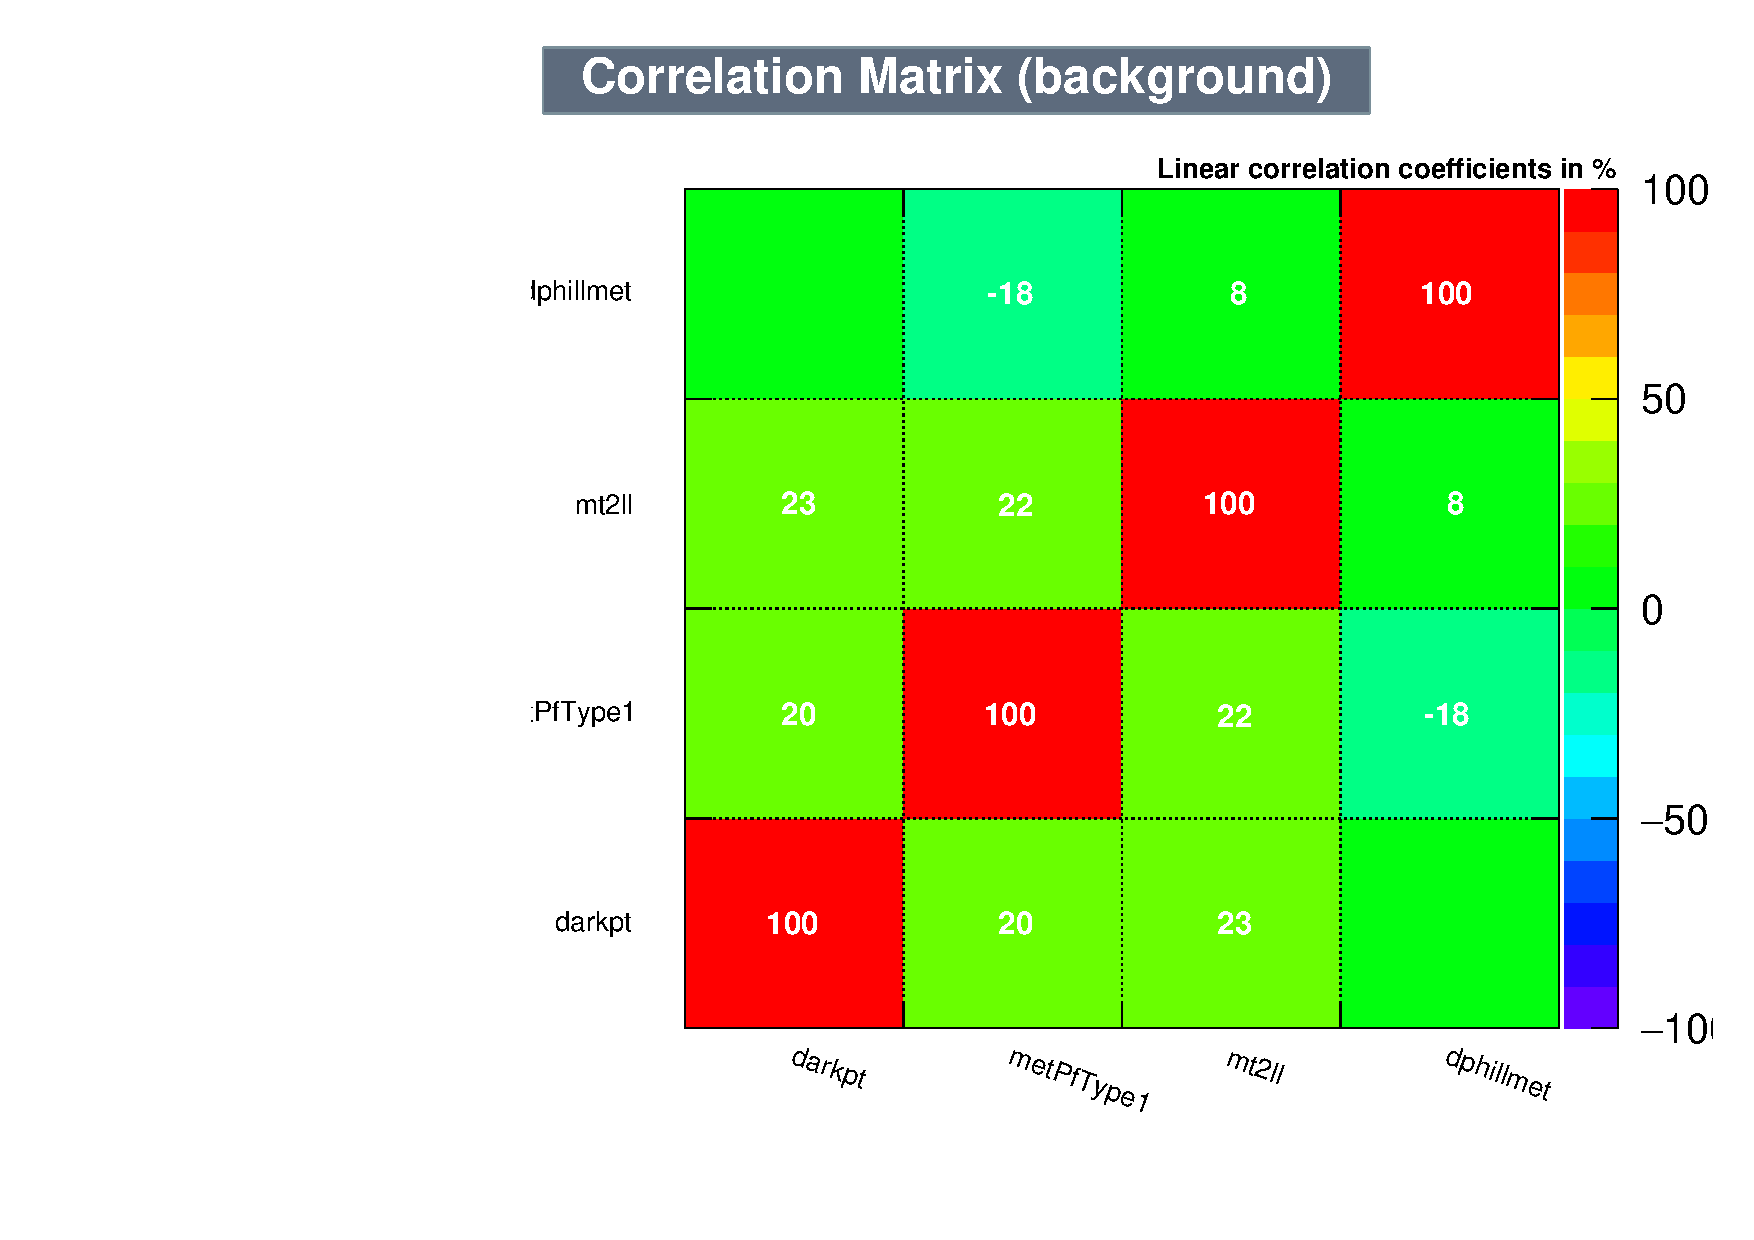
\includegraphics[width= 90pt, height= 90pt]{figs/newMVA/correlation_background_500GeV.pdf}
	}
   \end{minipage} \hfill
   \begin{minipage}[c]{.30\linewidth}
   	\centering{
		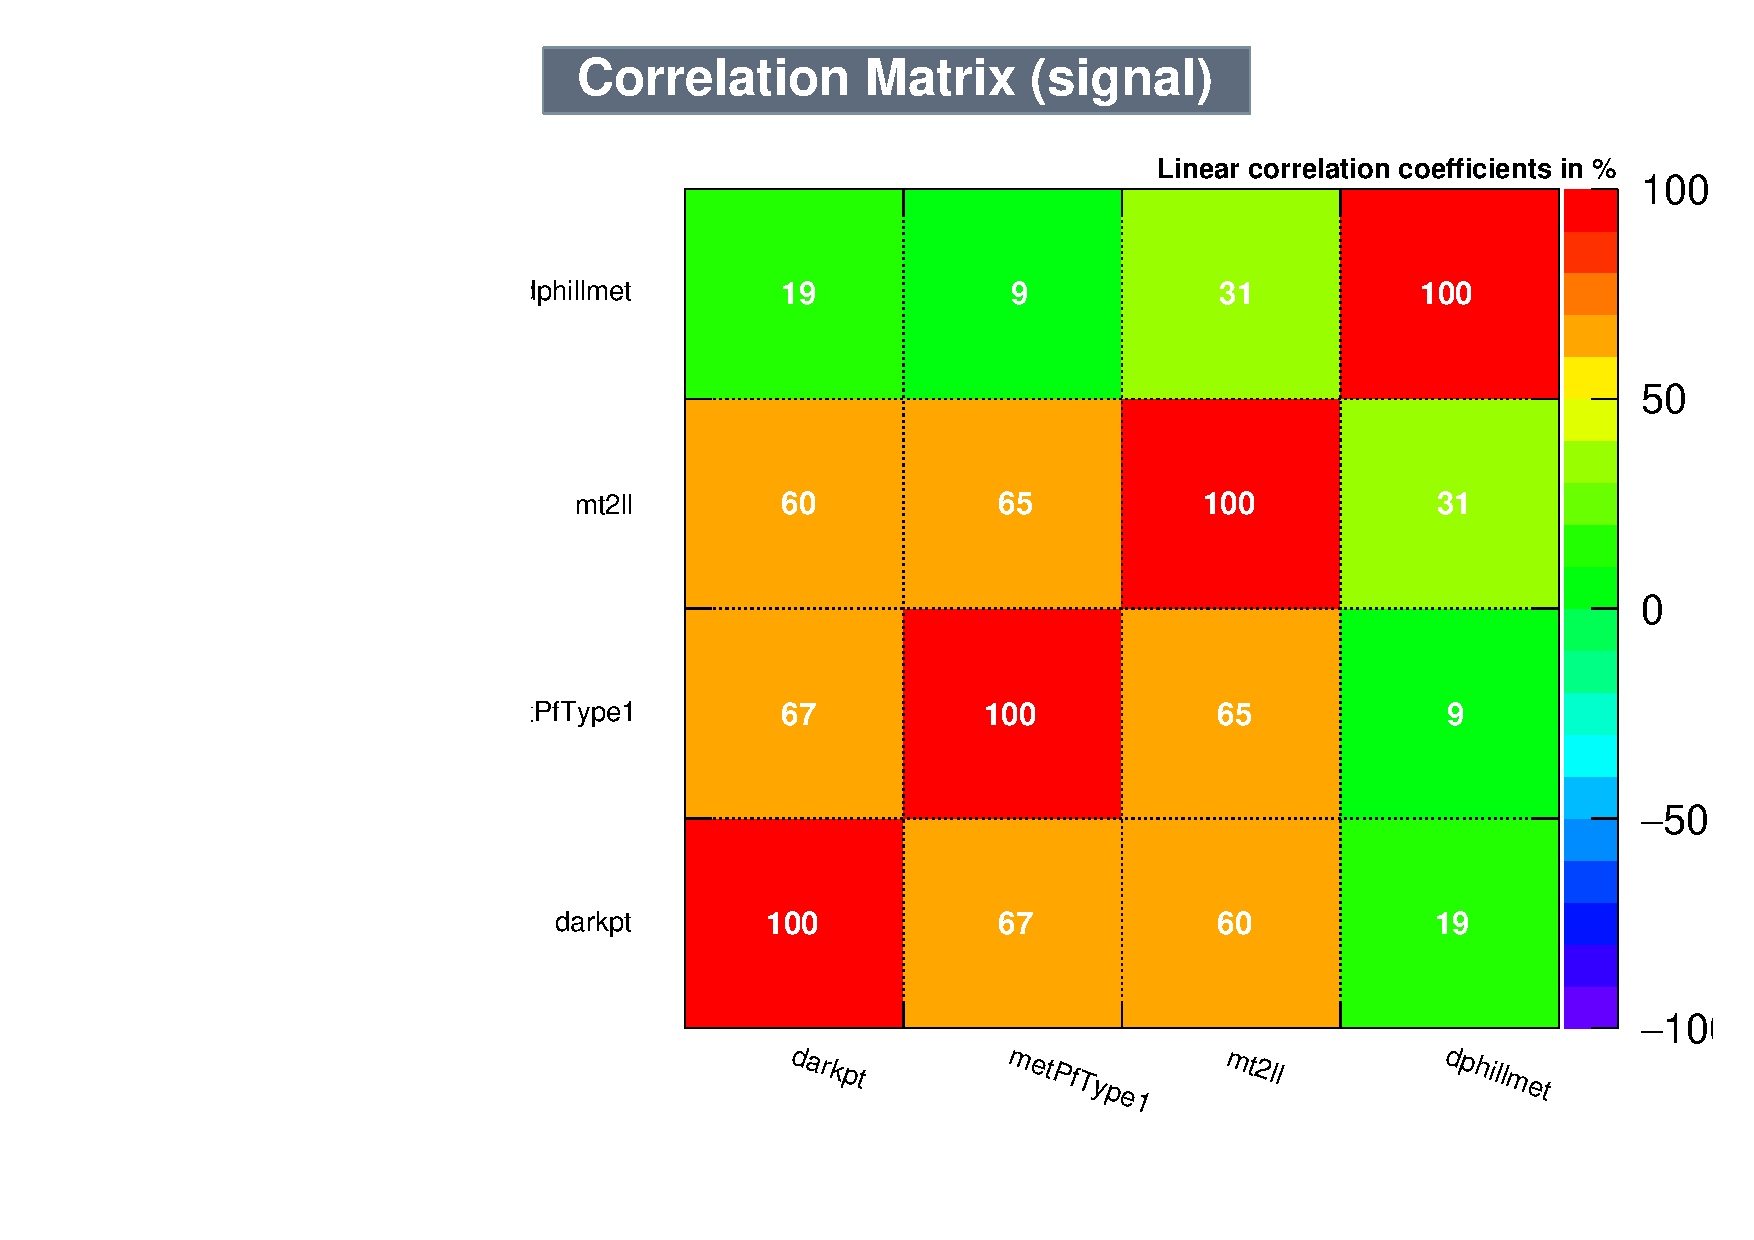
\includegraphics[width= 90pt, height= 90pt]{figs/newMVA/correlation_signal_500GeV.pdf} \\
	}
   \end{minipage} \hfill
   \begin{minipage}[c]{.30\linewidth}
   	\justifying
	The strongest correlations are obtained for the signal, between the $m_{T2}^{ll}$, the $E_T^{\text{miss}}$ and the dark $p_T$ variables.
   \end{minipage} \hfill
   %\begin{minipage}[c]{.30\linewidth}
   %	\begin{center} 
	%\resizebox{94pt} {!}{
	%\begin{tabular}{c|c|c}
	%	& & \\
	%	Variable & Sigmoid & Tanh \\
	%	& & \\
	%	\hline \hline
	%	& & \\
	%	$m_{T2}^{ll}$ & 17.75 & 14.83 \\
	%	dark $p_T$ & 4.62 & 6.64 \\
	%	$E_T^{\text{miss}}$ & 6.77 & 5.69 \\
	%	$\Delta \phi_{ll, E_T^{\text{miss}}}$ & 0.40 & 0.69 \\
	%	& & \\
	%\end{tabular}
	%}
	%\end{center}
   %\end{minipage} \hfill \vfill

\end{frame}


\begin{frame}{Artificial Neural Network III}

	\justifying
	Finally we can study the \textbf{actual output} of the different networks considered so far which is, at least for the moment, used in a simple count and count analysis. \vfill
	
	\hspace{4pt}
   \begin{minipage}[c]{.02\linewidth}
	\begin{exampleblock}{} \rotatebox{90}{ $m_\Phi$ = 10 GeV } \end{exampleblock}
   \end{minipage}
   \hspace{5pt}
	\begin{minipage}[c]{.44\linewidth}
   	\centering{
		\begin{exampleblock}{}{ \begin{center} Activation function 1 \end{center}} \end{exampleblock} \vspace{5pt}
		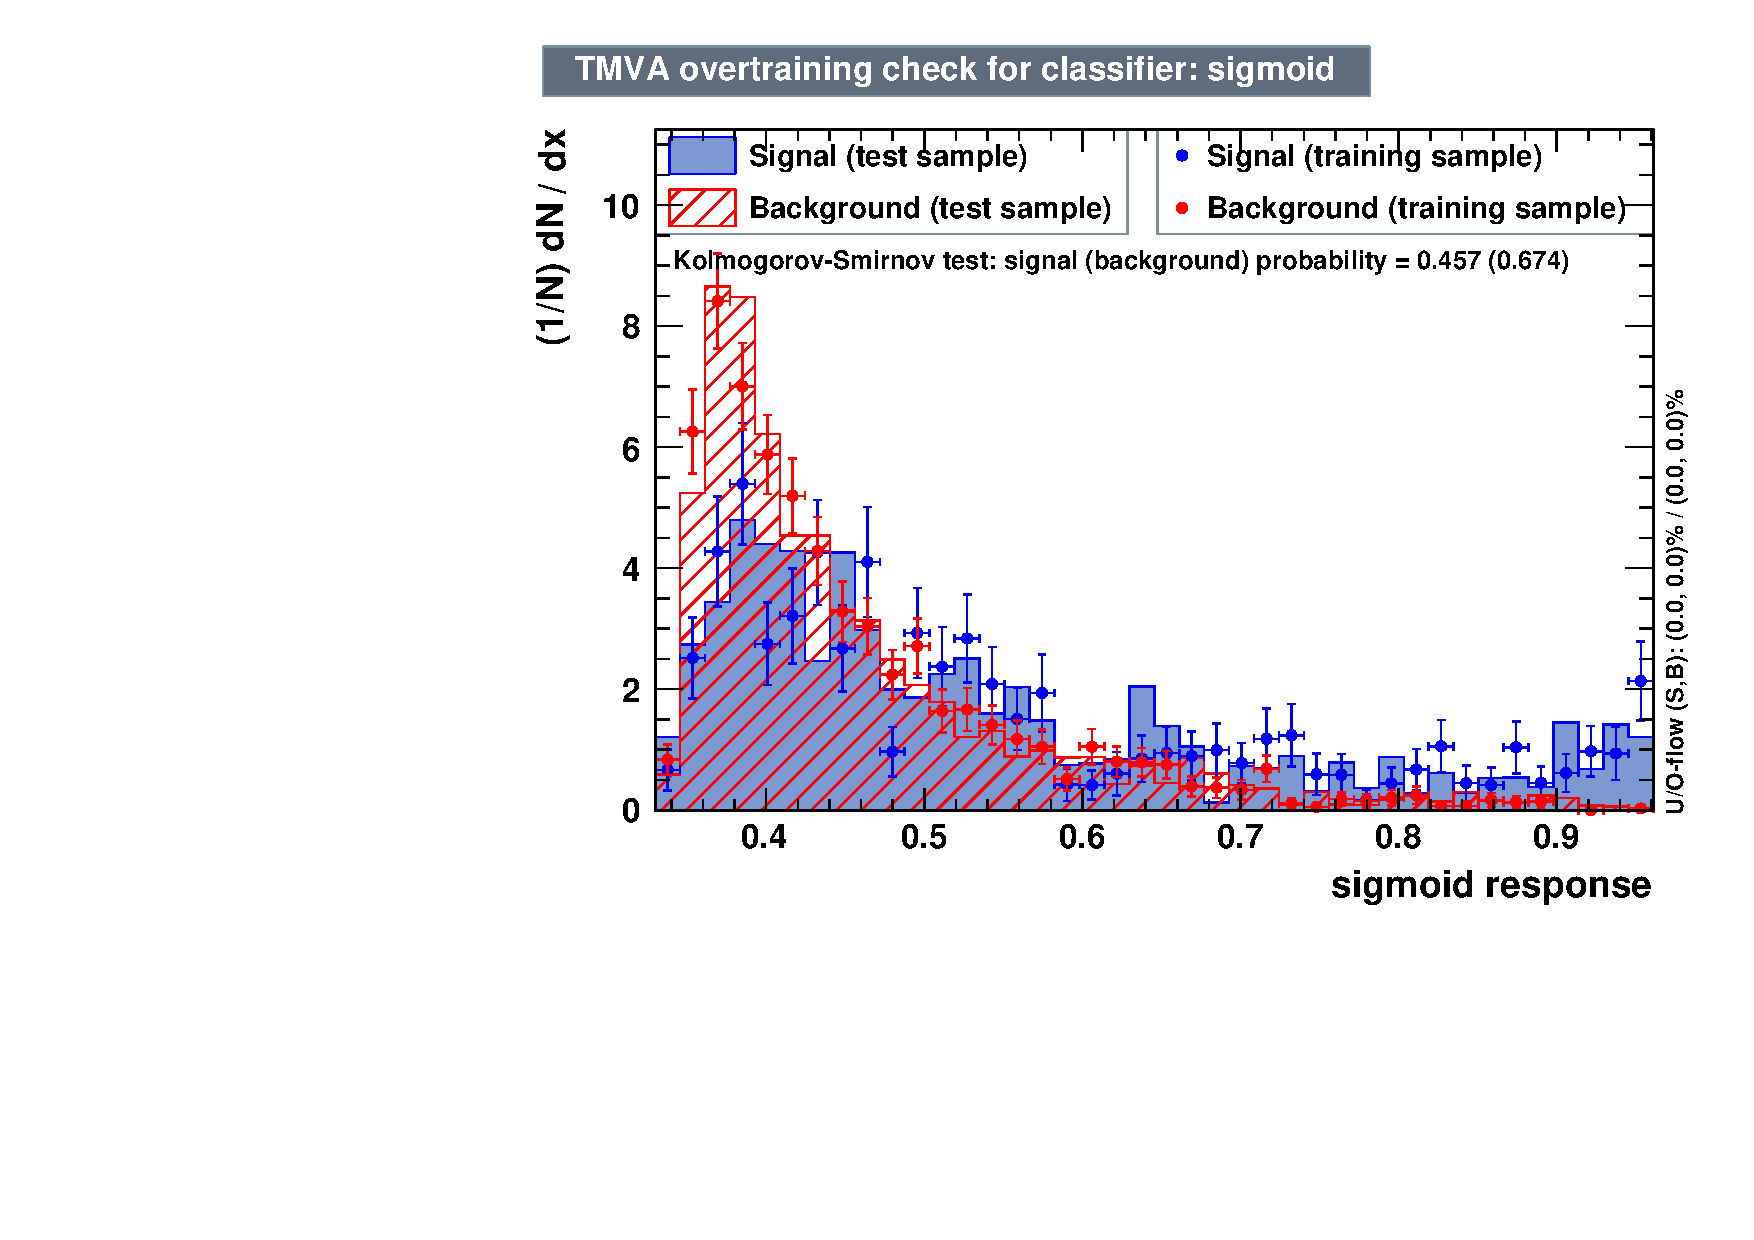
\includegraphics[width= 100pt, height= 72pt]{figs/newMVA/response_sigmoid_10GeV.pdf}
	}
   \end{minipage} \hfill
   \hspace{10pt}
   \begin{minipage}[c]{.44\linewidth}
   	\centering{
		\begin{exampleblock}{}{ \begin{center} Activation function 2 \end{center}} \end{exampleblock} \vspace{5pt}
		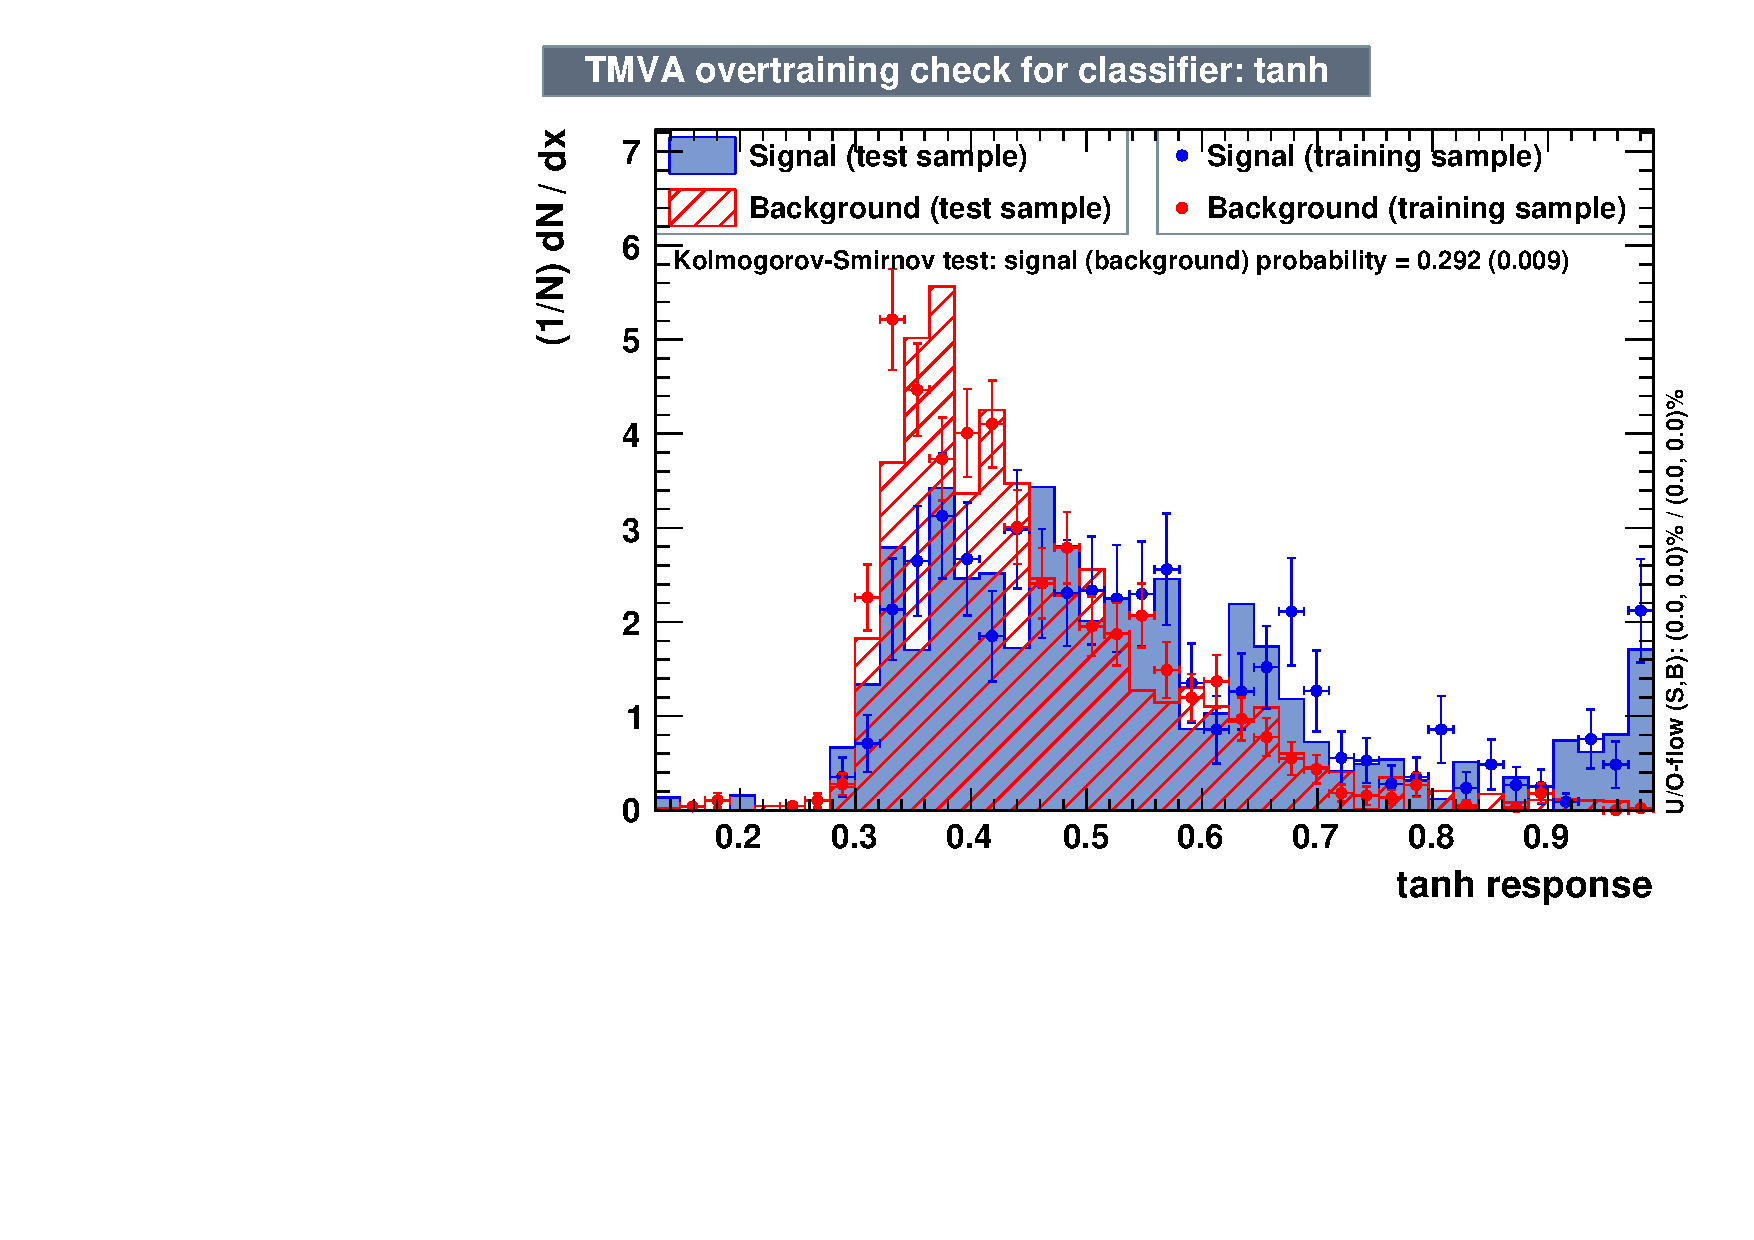
\includegraphics[width= 100pt, height= 72pt]{figs/newMVA/response_tanh_10GeV.pdf}
	}
   \end{minipage} \hfill \vfill
   
   	\hspace{4pt}
   \begin{minipage}[c]{.02\linewidth}
	\begin{exampleblock}{} \rotatebox{90}{ $m_\Phi$ = 500 GeV } \end{exampleblock}
   \end{minipage}
   \hspace{5pt}
	\begin{minipage}[c]{.44\linewidth}
   	\centering{
		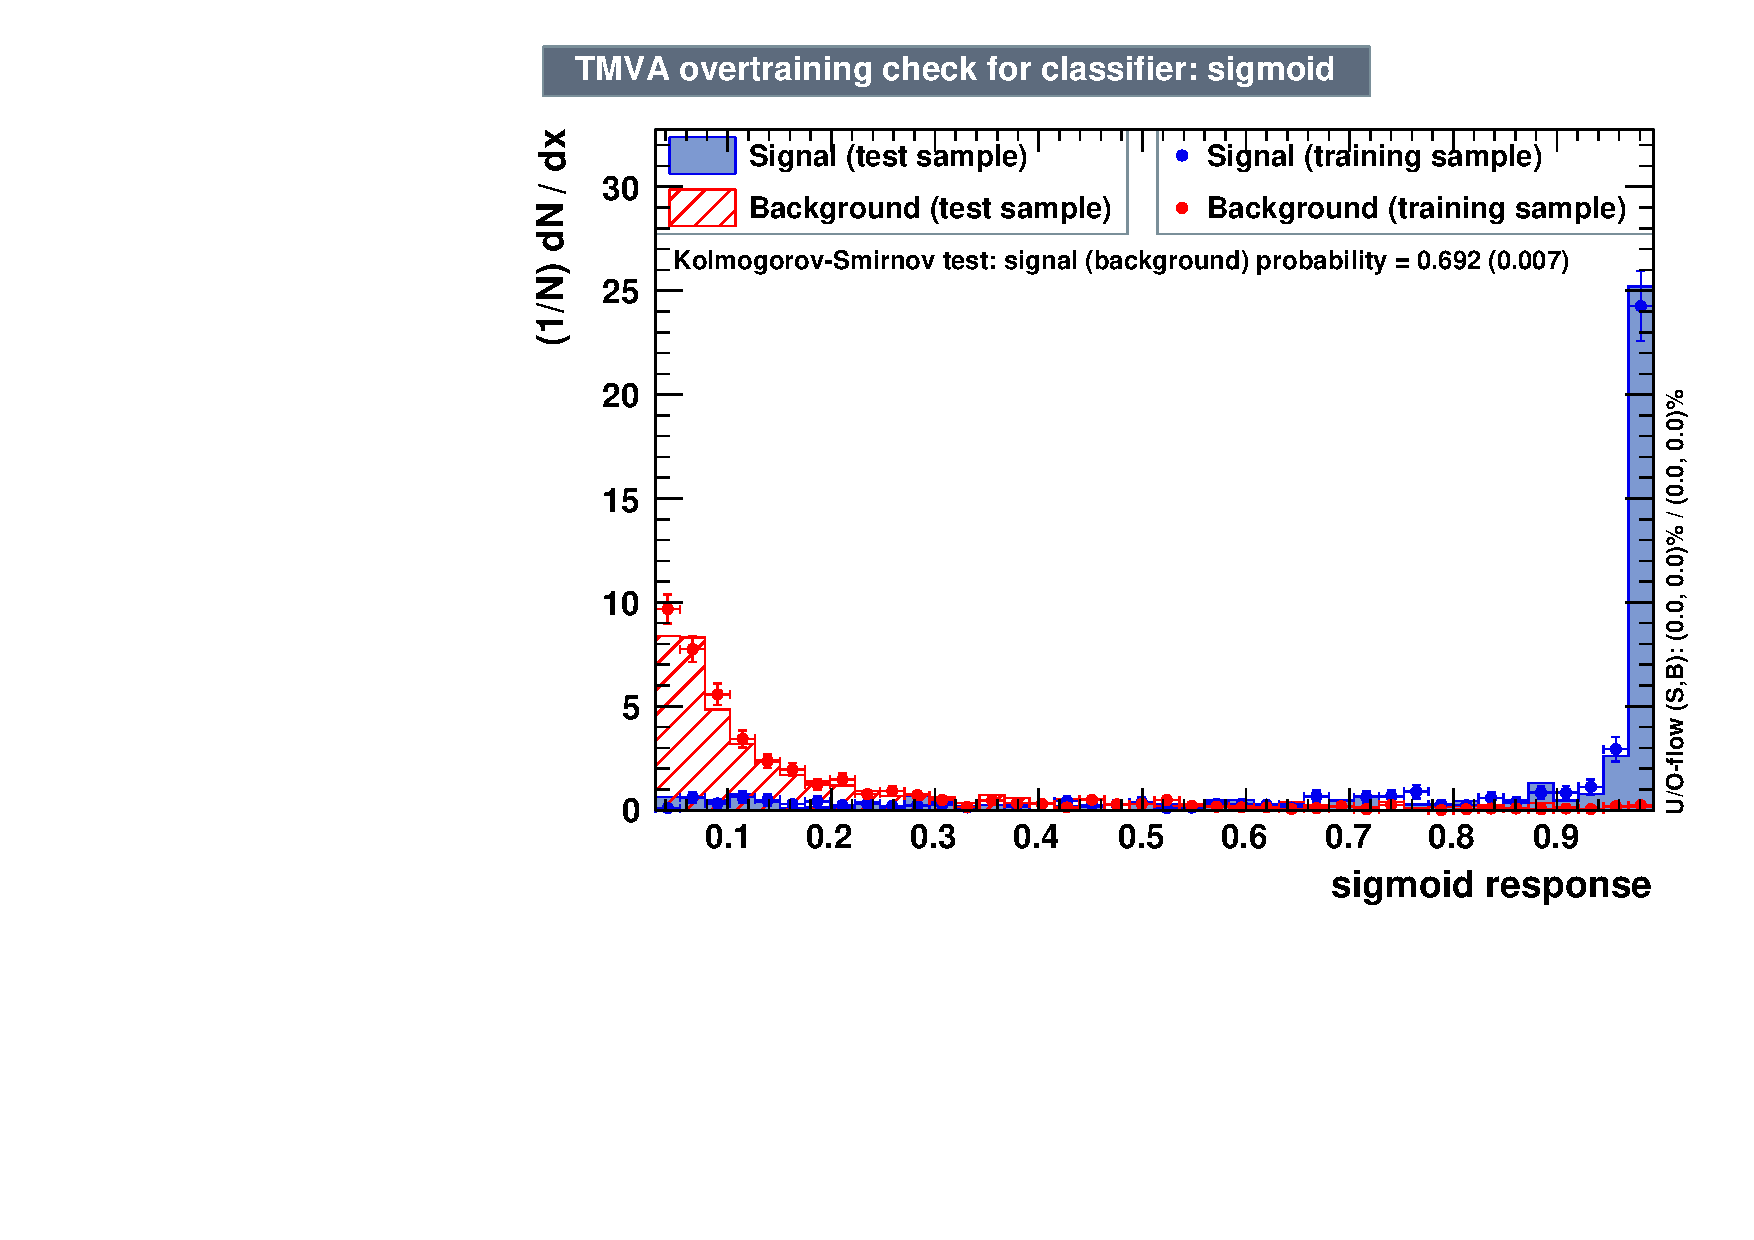
\includegraphics[width= 100pt, height= 72pt]{figs/newMVA/response_sigmoid_500GeV.pdf}
	}
   \end{minipage} \hfill
   \hspace{10pt}
   \begin{minipage}[c]{.44\linewidth}
   	\centering{
		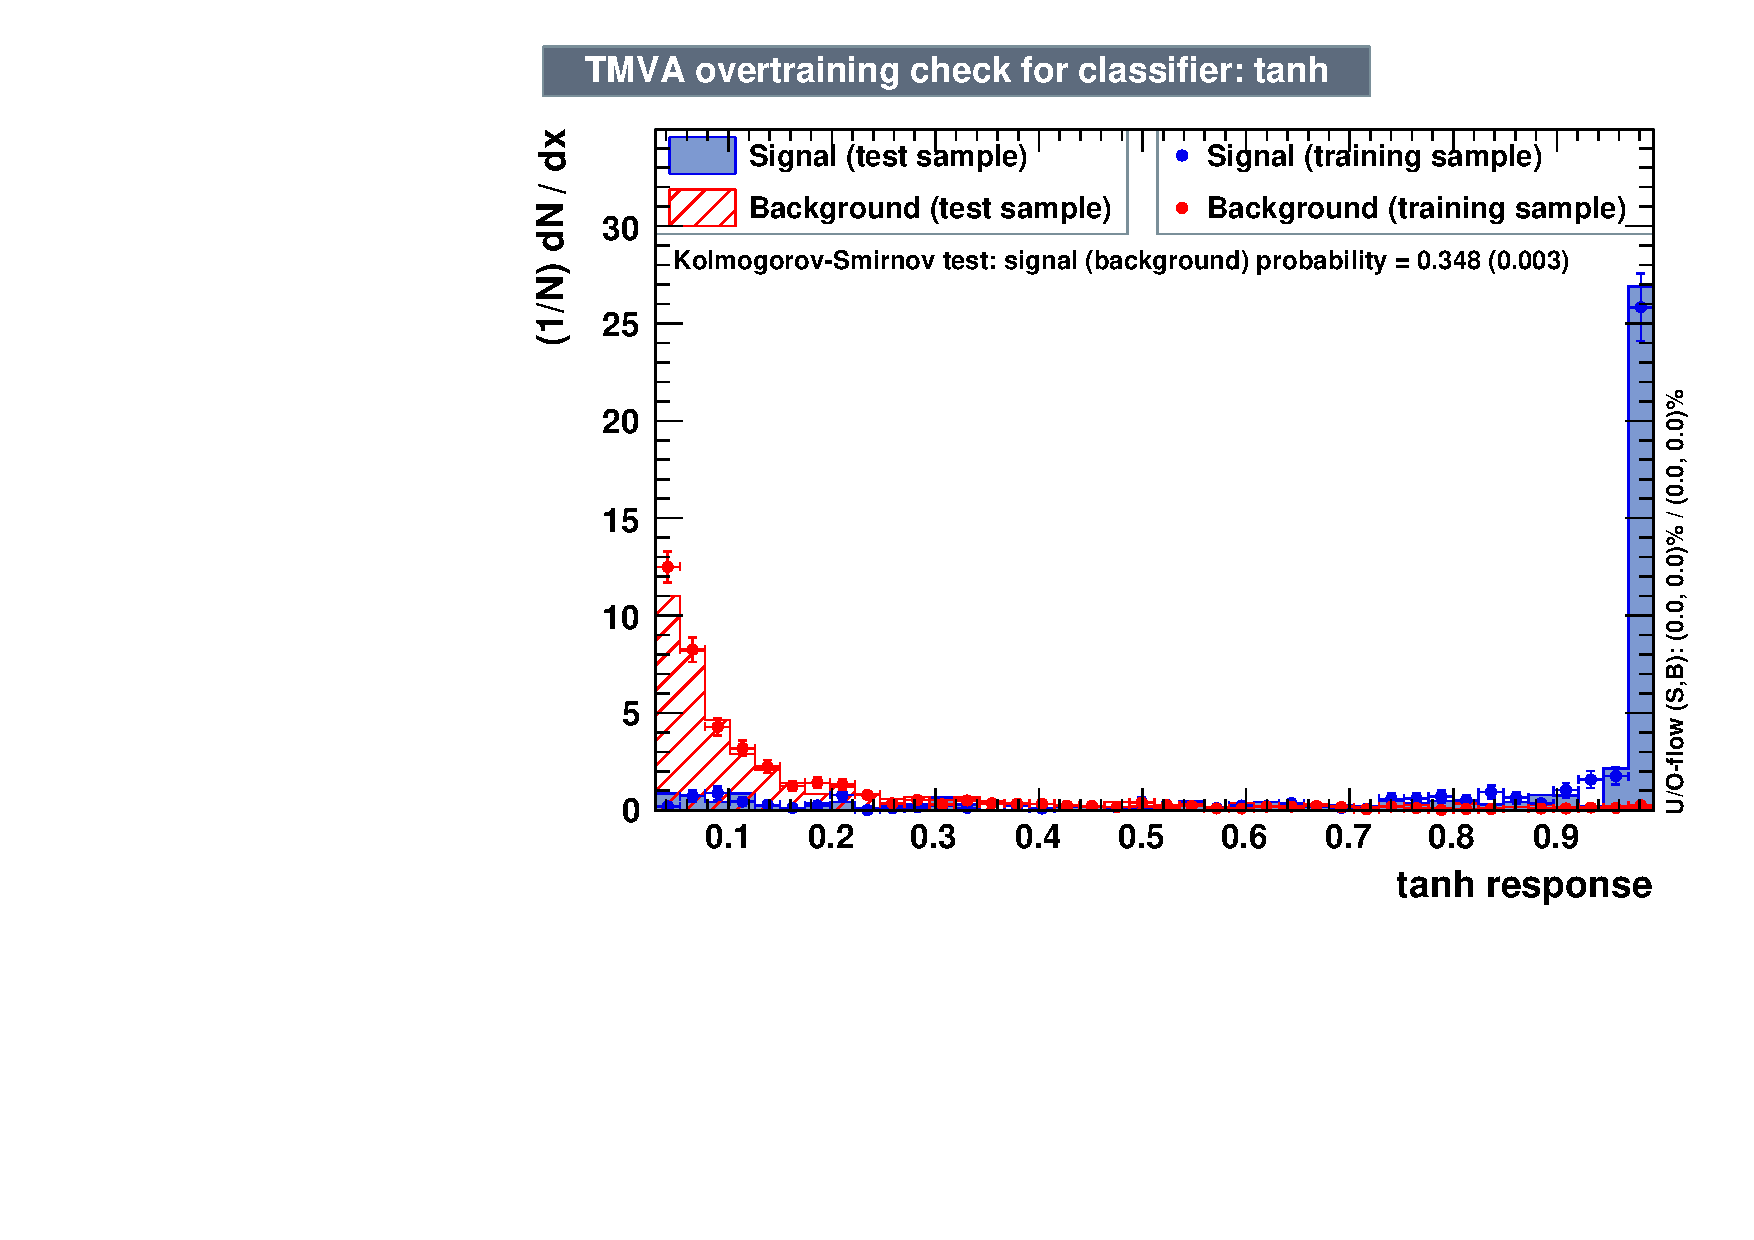
\includegraphics[width= 100pt, height= 72pt]{figs/newMVA/response_tanh_500GeV.pdf}
	}
   \end{minipage} \hfill \vfill
	
	\justifying
	We clearly observe a \textbf{better discrimination} of the output in the 500 GeV case, and the Kolmogorov-Smirnov test indicates that the first activation function output presents less overtraining. \vfill

\end{frame}


\begin{frame}{Systematic uncertainties}

	\justifying
	Several sources of \textbf{systematic uncertainties} have been considered, and can be classified into two different categories. The estimation of these systematics is a crucial point of the analysis since we need to get a precise idea about the error we are committing if we want to be able to make some conclusions about the eventual existence of dark matter. \vfill
	
	\begin{itemize}
	\justifying
	\item The \textbf{\color{mycolor}theoretical uncertainties\color{black}}, such as the Parton Density Functions normalization ($<$ 5\%) and shape ($<$ 3\%), and the high-order corrections of the MC simulations uncertainties. \vfill
	\item The \textbf{\color{mycolor}experimental uncertainties\color{black}} are usually coming from the detector itself. In this category are grouped several different uncertainties, such as:
	\vspace{-5pt}
		\begin{multicols}{2}
		\begin{itemize}
		\item Determination of the luminosity
		\item Lepton RECO and ID normalization ($<$ 2\%) and shape ($<$ 1\%)
		\item B-tagging efficiency normalization ($<$ 7\%) and shape ($<$ 7\%)
		\item Jet energy scale normalization ($<$ 4\%) and shape ($<$ 10\%)
		\item $E_T^{\text{miss}}$ modeling and resolution 
		%\item Top $p_T$ reweighting 
		\item Non-prompt (30\%), $t \bar t$ (15\%) and Drell-Yan normalizations (7\%)
		\end{itemize}
		\end{multicols}
	\end{itemize} \vfill
	
	\justifying
	The other backgrounds estimated directly from Monte Carlo get an usual 50\% systematic uncertainty associated. All of the previously mentioned systematics have of course been taken into account when plotting the limits of the analysis (and for most of them, we did considered both their normalization and shape). \vfill

\end{frame}


\begin{frame}{Yields table}

	\justifying 
	We can now represent the yields obtained for the different backgrounds with the associated systematics, for the different background processes and different dark matter mediator mass points (and therefore, different neural networks). \vfill
	
	\begin{minipage}[c]{.48\linewidth}
	
	\begin{center}
	
	\begin{exampleblock}{}{ \begin{center} 10 GeV scalar (ANN output $>$ 0.75) \end{center}} \end{exampleblock} \vspace{6pt}
	
	\resizebox{170pt} {!}{
	\begin{tabular}{c|c|c|c}
	 	& & & \\
		Process & Yields & Statistical error & Systematic error \\
		& & & \\
		\hline \hline
		& & & \\
		$t \bar t$ & 11.08 & 0.18 & 1.72 \\
		Non-prompt & 1.30 & 0.92 & 0.39 \\
		ttV & 0.75 & 0.03 & 0.19 \\
		Single top & 0.48 & 0.07 & 0.16 \\
		Drell-Yan & 0.46 & 0.35 & 0.34 \\
		WW & 0.02 & 0.02 & 0.02 \\
		& & & \\
		\hline
		& & & \\
		Total background & 14.09 & 1.00 & 1.81 \\
		& & & \\
		\hline
		& & & \\
		Signal & 3.21 & 0.18 & 2.28 \\
		Total with signal & 17.30 & 1.02 & 2.91 \\
		& & & \\
		\hline
		& & & \\
		Data & 10 & - & - \\
		& & & \\
	\end{tabular}
	} 
	
	\end{center}

	\end{minipage} \hfill
	\begin{minipage}[c]{.48\linewidth}
	
	\begin{exampleblock}{}{ \begin{center} 500 GeV scalar (ANN output $>$ 0.98) \end{center}} \end{exampleblock} \vspace{6pt}
	
	\resizebox{170pt} {!}{
	\begin{tabular}{c|c|c|c}
	 	& & & \\
		Process & Yields & Statistical error & Systematic error \\
		& & & \\
		\hline \hline
		& & & \\
		$t \bar t$ & 1.82 & 0.14 & 0.28 \\
		Non-prompt & 0.00 & 0.00 & 0.00 \\
		ttV & 0.57 & 0.03 & 0.15 \\
		Single top & 0.12 & 0.06 & 0.04 \\
		Drell-Yan & 0.00 & 0.00 & 0.00 \\
		WW & 0.01 & 0.01 & 0.01 \\
		& & & \\
		\hline
		& & & \\
		Total background & 2.52 & 0.16  & 0.32 \\
		& & & \\
		\hline
		& & & \\
		Signal & 0.03 & 0.01 & 0.01 \\
		Total with signal & 2.55 & 0.16 & 0.32 \\
		& & & \\
		\hline
		& & & \\
		Data & 2 & - & - \\
		& & & \\
	\end{tabular}
	} 
	
	\end{minipage} \hfill \vfill
	
	\justifying
	$\rightarrow$ The yields tables for the pseudoscalar mediator can be found in the backup. \vfill

\end{frame}


\begin{frame}{Scalar limits}

	\justifying
	We can now represent the \textbf{limits} of the analysis, for both the scalar and pseudoscalar mediators. \\ \vspace{8pt} The limit plots consist in plotting the value of the upper limit on the cross-section for which we expect to get some sensitivity, divided by the theoretical cross-section. This way, obtaining a value smaller than 1 for a given mass point then means that with the luminosity considered, we would \textbf{expect to get some sensitivity} to the signal. \vfill

	\hspace{4pt}
   \begin{minipage}[c]{.02\linewidth}
	\begin{exampleblock}{} \rotatebox{90}{ Scalar mediator } \end{exampleblock}
   \end{minipage}	
   \hspace{5pt}	
   \begin{minipage}[c]{.40\linewidth}
   	\begin{center}
		\vspace{15pt}
		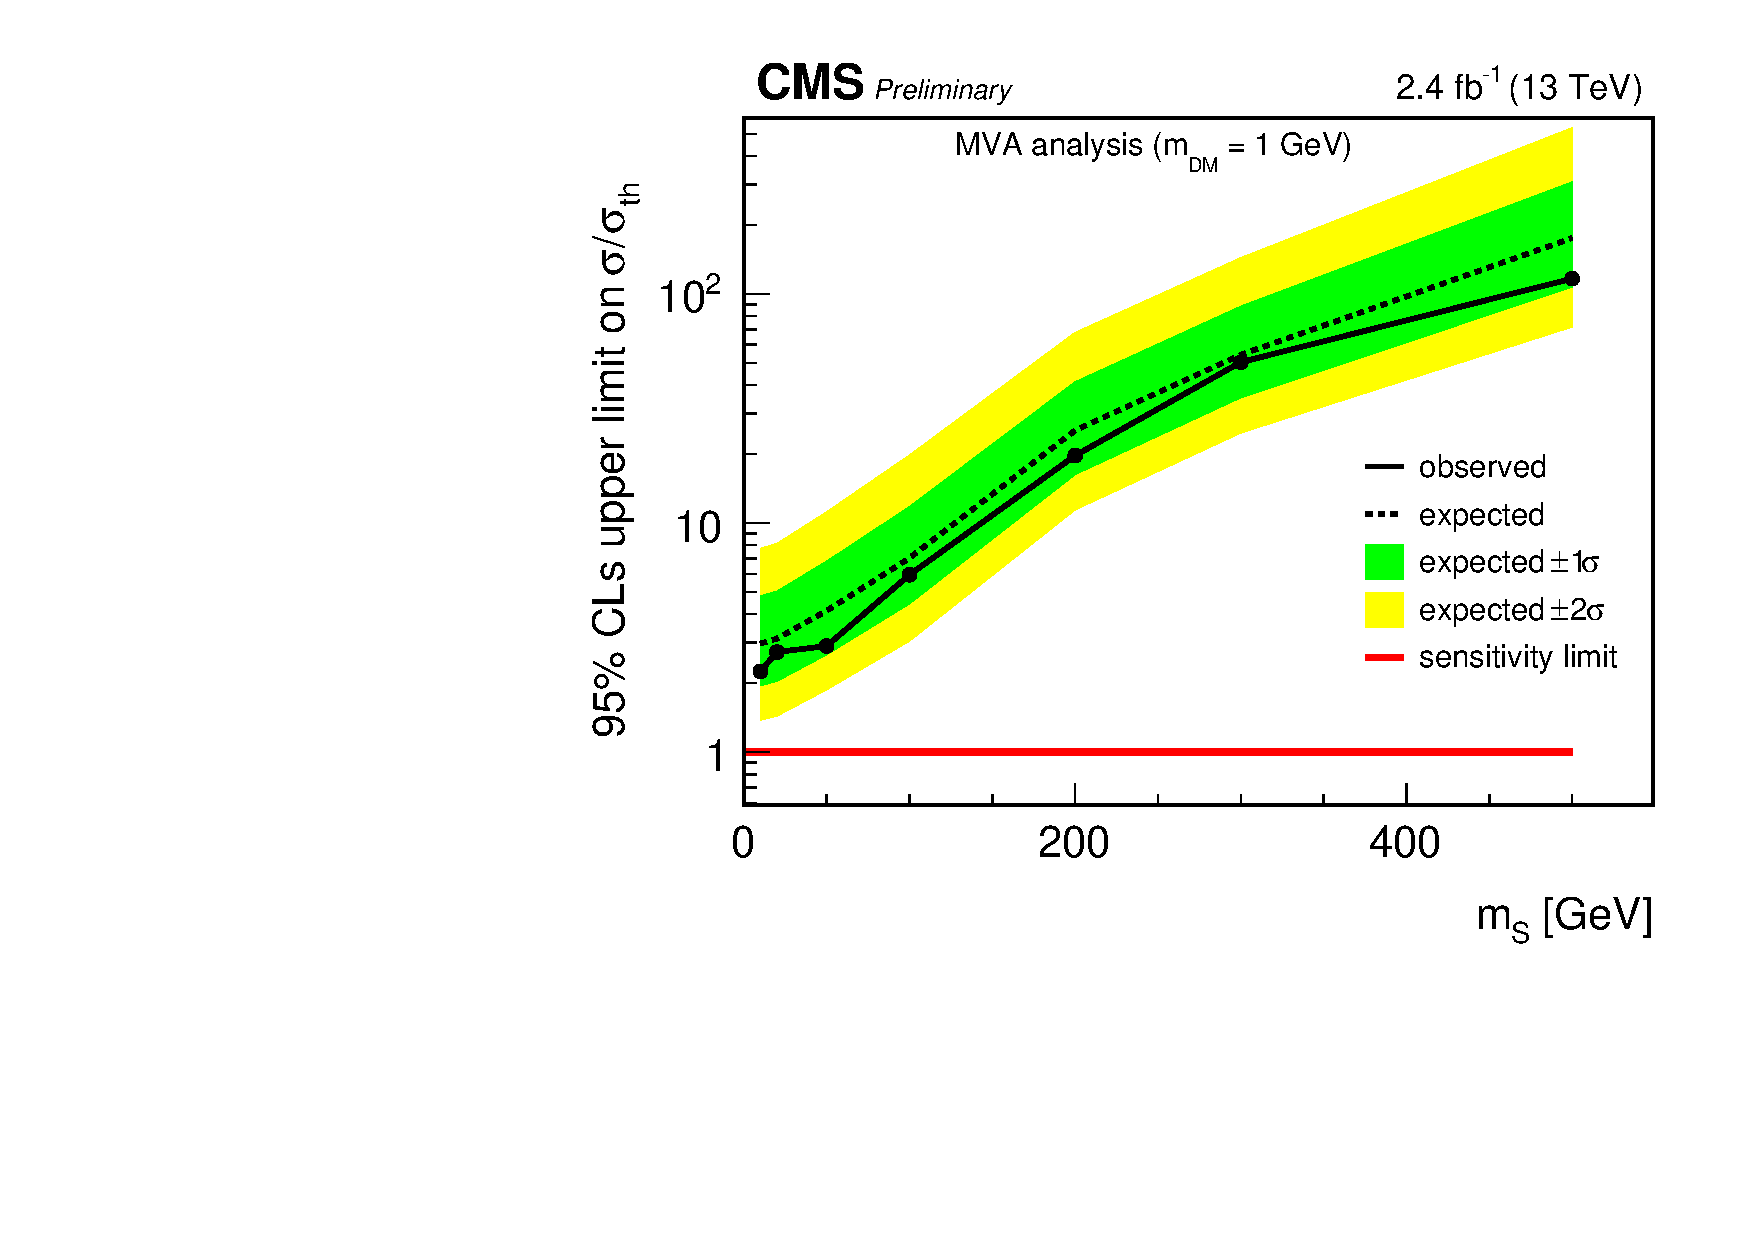
\includegraphics[width=130pt, height=130pt]{figs/limits_scalar.pdf}
	\end{center}
   \end{minipage} \hfill
    \begin{minipage}[c]{.52\linewidth}
   	\begin{center}
	\resizebox{175pt} {!}{
   	\begin{tabular}{c|c|c|c}
		& & & \\
		$m_S$ [GeV]& Best AAN cut & Expected limit & Observed limit \\ 
		& & & \\ 
		\hline \hline
		& & & \\
		10 & 0.75 & 2.99 & 2.22 \\
            	20 & 0.80 & 3.12 & 2.73 \\
            	50 & 0.90 & 4.14 & 2.90 \\
            	100 & 0.90 & 7.03 & 5.94 \\
            	200 & 0.90 & 25.37 & 19.69 \\
            	300 & 0.80 & 54.25 & 50.34 \\
            	500 & 0.98 & 175.50 & 116.65 \\
		& & & \\
          \end{tabular}
          }
          \end{center}
   \end{minipage} \hfill \vfill
   
   The green and yellow lines on the plot correspond to the 1 and 2$\sigma$ confidence intervals for the value of the expected limits. \vfill

\end{frame}


\begin{frame}{Pseudoscalar limits}

	\hspace{4pt}
   \begin{minipage}[c]{.02\linewidth}
	\begin{exampleblock}{} \rotatebox{90}{ Pseudoscalar mediator } \end{exampleblock}
   \end{minipage}	
   \hspace{5pt}	
   \begin{minipage}[c]{.40\linewidth}
   	\begin{center}
		\vspace{15pt}
		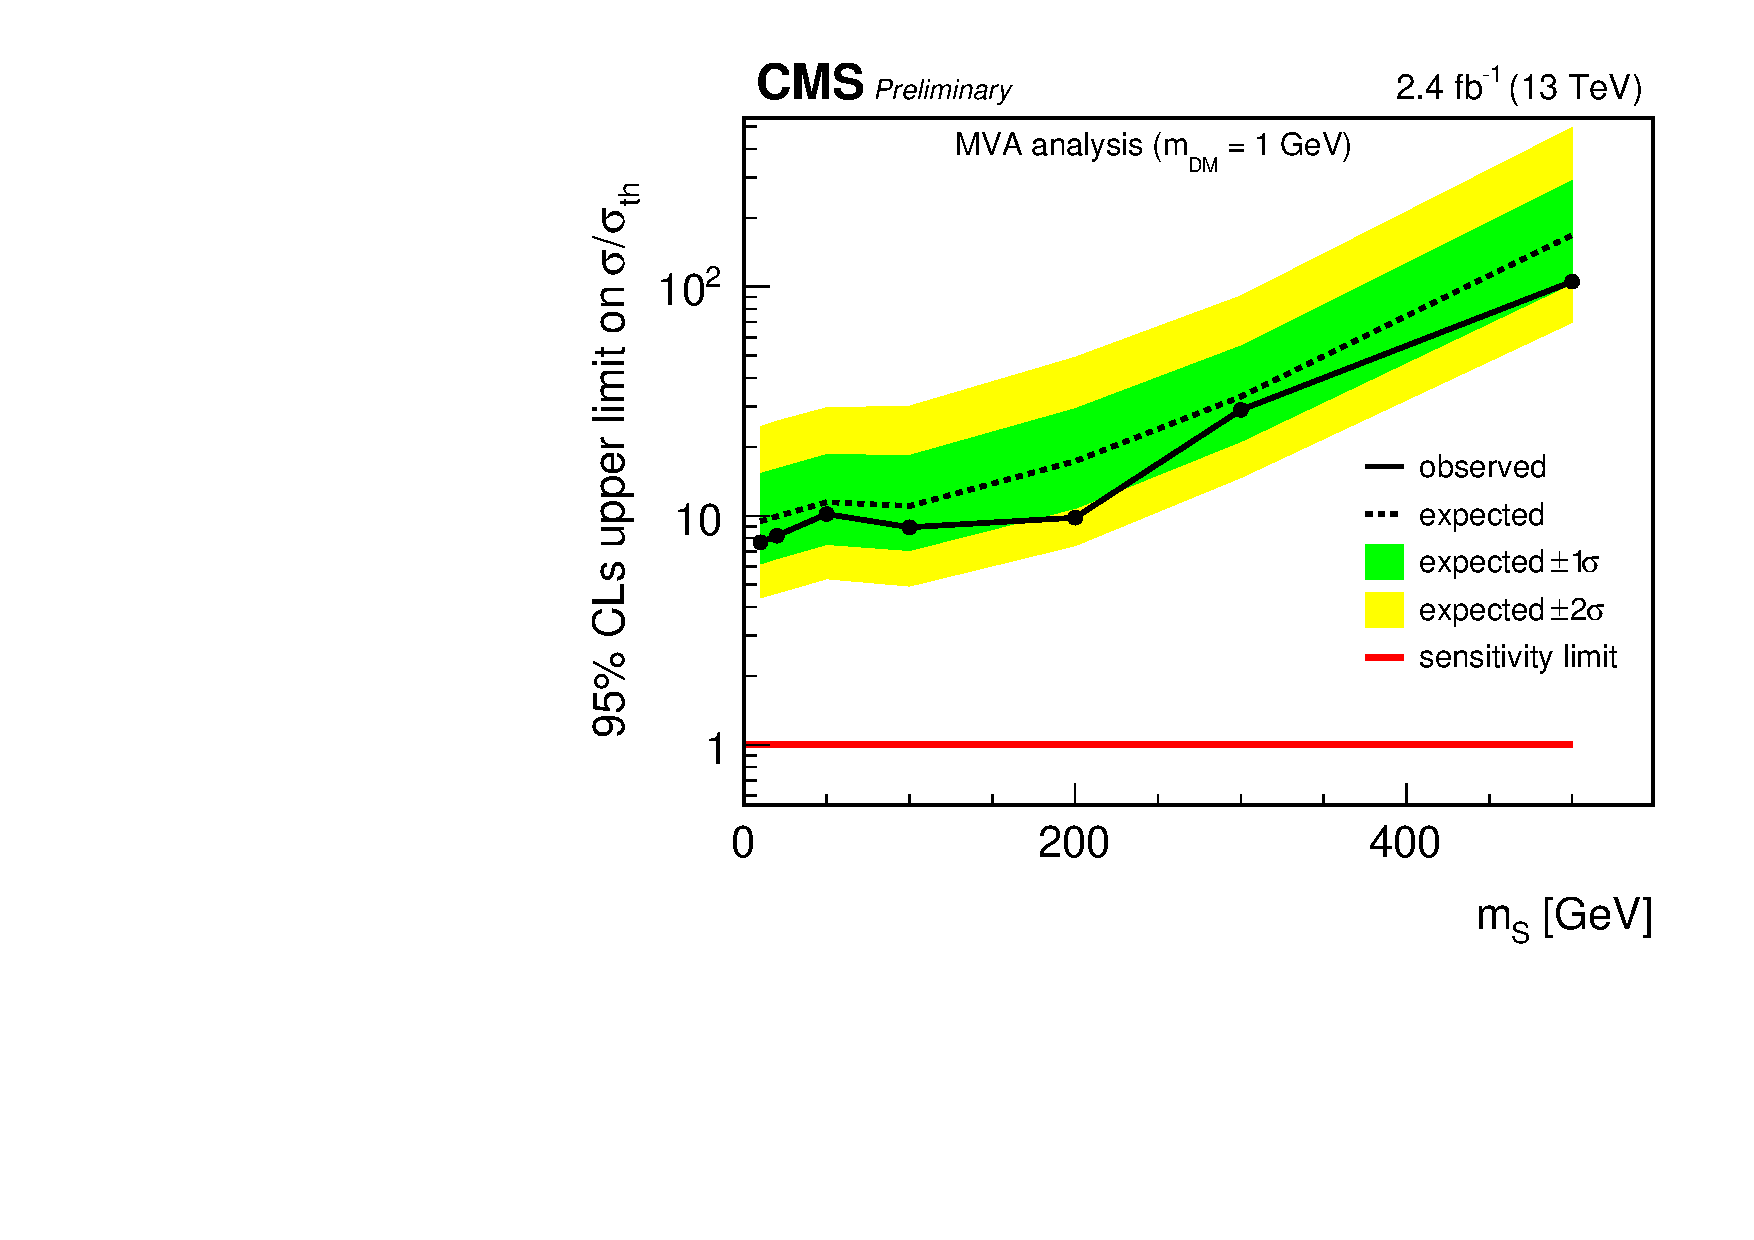
\includegraphics[width=130pt, height=130pt]{figs/limits_pseudo.pdf}
	\end{center}
   \end{minipage} \hfill
    \begin{minipage}[c]{.52\linewidth}
   	\begin{center}
	\resizebox{175pt} {!}{
   	\begin{tabular}{c|c|c|c}
		& & & \\
		$m_P$ [GeV]& Best ANN cut & Expected limit & Observed limit \\ 
		& & & \\ 
		\hline \hline
		& & &  \\
		10 & 0.80 & 9.47 & 7.66 \\
            	20 & 0.85 & 9.94 & 8.18 \\
            	50 & 0.85 & 11.47 & 10.18 \\
            	100 & 0.90 &11.03 & 8.91 \\
            	200 & 0.95 & 17.31 & 9.81 \\
            	300 & 0.80 & 33.12 & 28.98 \\
            	500 & 0.98 & 167.94 & 105.27 \\
		& & & \\
          \end{tabular}
          }
          \end{center}
   \end{minipage} \hfill 
   
   \vspace{-10pt}
   \begin{block}{}
   \justifying
   \vspace{5pt}
	With our analysis and considering for the moment the 2.4 fb$^{-1}$ blinded dataset, we \textbf{cannot exclude} any dark matter production model. \vspace{5pt}
	\end{block} \vfill
	
	\justifying
	However, we expect to be \textbf{able to exclude the 10 and 20 GeV scalar mediators} once considering the complete 2016 dataset, since we know that our sensitivity scales with the change in luminosity. \vfill
   

\end{frame}


\begin{frame}{Conclusions}

	\justifying
	A search for dark matter production in association with top quark pairs in the dilepton final state has been performed. The analysis has been made using a 2.4 fb$^{-1}$ blinded dataset for the signal region, and the complete 35.9 fb$^{-1}$ dataset for the control regions, both taken by the CMS detector at CERN, at a center of mass energy of $\sqrt{s} = 13$ TeV. \vfill
	
	The results obtained \textbf{do not allow us to exclude any dark matter production model} so far, with the limited luminosity considered, but we do \textbf{expect to be able to exclude the 10 and 20 GeV scalar mediators} when unblinding the analysis. \vfill
	
	We did think about several ways we have to improve the analysis. First of all, a \textbf{better understanding} of the different \textbf{backgrounds} (mainly the $t \bar t$) and the different \textbf{systematics} is a crucial point since studying them in more detail and reducing them would allow us to improve our results. Moving to a complete shape study of the output of the MVA instead of performing a simple cut and count analysis is also expected to improve the final results, and will be done as soon as possible. \vfill

\end{frame}



\begin{frame}{}

	\centering
	\huge{\textbf{\color{mycolor} Thank you  \color{black}}} \newline
	\LARGE{\textbf{\color{mycolor} for your attention! \color{black}}} \vfill

	Any questions? \vfill

\end{frame}

\appendix
	\backupbegin
	
\begin{frame}{Top reconstruction addendum}

   	\justifying
	We can get 6 different equations from the kinematics expected for our signal. \vspace{5pt}
	
	\begin{minipage}[c]{.30\linewidth}
        \begin{equation*}
     	\begin{cases}
        		%M(b_1 + \nu_1 + l_1) = M_t \\
		%M(b_2 + \nu_2 + l_2) = M_t \\
		M(b_1 + W_1) = M_t \\
		M(b_2 + W_2) = M_t \\
     	\end{cases}
	\end{equation*}
	\justifying
	...because both the tops produced decay to a bottom and a W boson. \\
   \end{minipage} \hfill
   \hspace{8pt}
   \begin{minipage}[c]{.3\linewidth}
   	\begin{equation*}
     	\begin{cases}
        		M(\nu_1 + l_1) = M_W \\
		M(\nu_2 + l_2) = M_W \\
     	\end{cases}
	\end{equation*}
	\justifying
	...because we only consider the leptonic decay of the W in this analysis. \\
   \end{minipage} \hfill
   \hspace{8pt}
   \begin{minipage}[c]{.3\linewidth}
   	\begin{equation*}
     	\begin{cases}
        		\nu_{1_x} + \nu_{2_x} = (E_T^{miss})_x \\
		%\nu_{1_y} + \nu_{2_y} = $\cancel{\textit{E}}$_{{T}_y} \\
		\nu_{1_y} + \nu_{2_y} = (E_T^{miss})_y \\
     	\end{cases}
	\end{equation*}
	\justifying
	...at least if we assume that the $E_T^{\text{miss}}$ is coming from the neutrinos only. \\
   \end{minipage} \hfill

	\vspace{13pt}

	\justifying
	$\rightarrow$ We have 6 equations and 6 unknowns (the three components of the momenta of the two neutrinos), meaning that this is a problem which can be solved. However, we have to find a way to correct the efficiency drop appearing when considering the signal, since the last hypothesis is not correct in this case (the $E_T^{\text{miss}}$ is not coming only from the neutrinos). \vfill
	
	\begin{block}{}
   	\justifying
	%\item However, since some of the parameters of the previous equations are not well known or precisely determined, this method is not expected to give us the exact momentum of the dark matter mediator, but will return its probable value. The top reconstruction therefore needs to be understood as a statistical problem.
	\vspace{5pt}
	This variable is expected to give some discrimination between the usual $t \bar t$ and our signal because in the dark matter case, we expect the $p_T$ of the tops to be higher, since they will be accommodating for the extra missing transverse energy which appears (at least, if we manage to correct the efficiency drop issue since in this latest case, the previous equations are actually not exactly true). \vspace{5pt}
	\end{block} \vfill

\end{frame}


\begin{frame}{$E_T^{\text{miss}}$ variable definition}

   	\justifying
	The $E_T^{\text{miss}}$, the missing transverse energy, corresponds to the imbalance of vector momentum in the plane perpendicular to the beam direction. It is defined in the following way: \vfill
	
	\begin{equation*}
		E_T^{\text{miss}} = -\sum_i{\overrightarrow{p}_T(i)}
	\end{equation*} \vfill
	
	\justifying
	We have to consider the missing \underline{transverse} energy and not directly the missing energy simply because the LHC is a proton-proton collider, and because each proton has three quarks (and the totat energy is distributed between these quarks in unknown proportions). This means that, for any given collision, we cannot actually know the exact initial longitudinal energy of collision. However, we do know that the initial transverse energy of the collision is equal to 0, so we can only calculate differences in transverse energy. \vfill
	
	\begin{block}{}
	\vspace{5pt}
	\justifying
	We expect this variable to give some discrimination between the $t \bar t$ and our signal because we know that the eventual dark matter particles produced should escape the detector while being undetected, since they almost do not interact with ordinary matter.  The only way to detect the production of this kind of particle is therefore to look at the missing transverse energy. \vspace{5pt}
	\end{block} \vfill

\end{frame}


\begin{frame}{$\Delta \Phi_{ll, E_T^{\text{miss}}}$ variable definition}

   	\justifying
	This variable corresponds to the angle in the $\Phi$ plane, between the two leptons coming from the tops and the missing transverse energy.  \vfill
   
   \begin{minipage}[c]{.3\linewidth}
   	\centering{
	\begin{exampleblock}{}{ \begin{center} $t \bar t$ background \end{center}} \end{exampleblock} \vspace{5pt}
		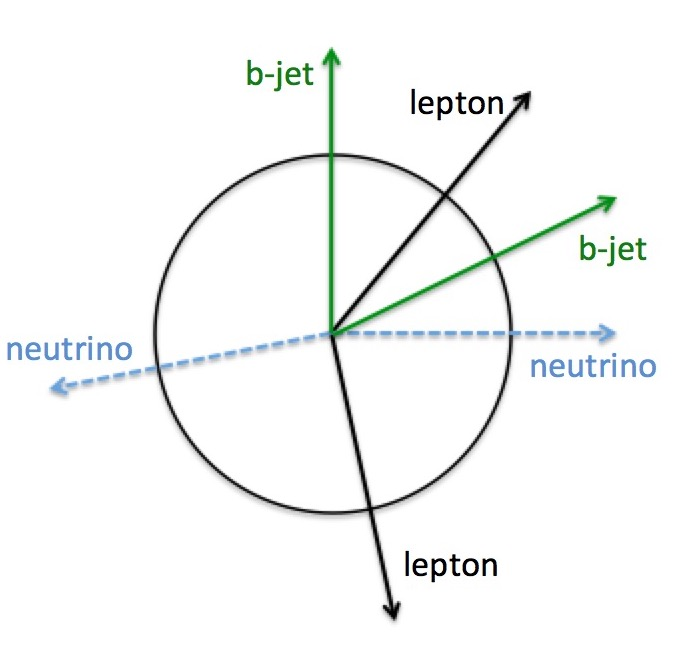
\includegraphics[width= 100pt, height= 100pt]{figs/deltaphi_mine.jpg}
	}
   \end{minipage} \hfill
   \begin{minipage}[c]{.3\linewidth}
   	\centering{
	\begin{exampleblock}{}{ \begin{center} $t \bar t$ + DM (low $m_\Phi$) \end{center}} \end{exampleblock} \vspace{5pt}
		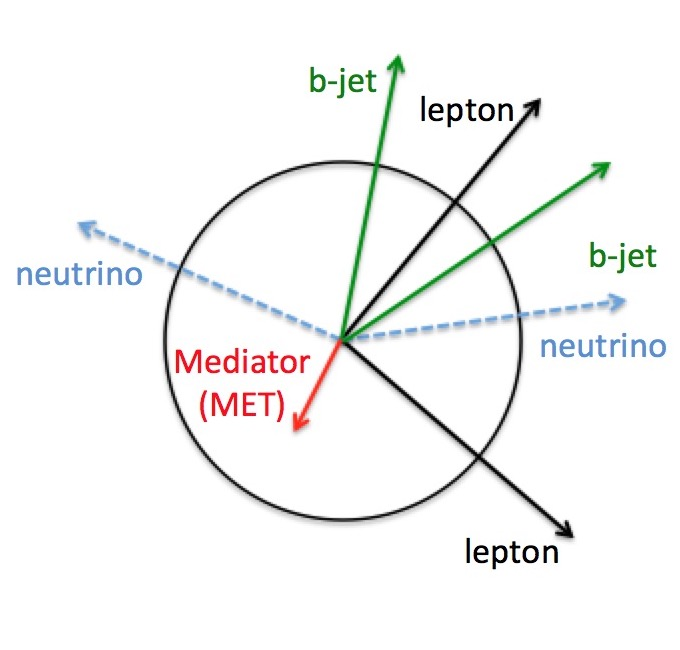
\includegraphics[width= 100pt, height= 100pt]{figs/deltaphi_low_mine.jpg} \\
	}
   \end{minipage} \hfill
   \begin{minipage}[c]{.3\linewidth}
   	\centering{
	\begin{exampleblock}{}{ \begin{center} $t \bar t$ + DM (high $m_\Phi$) \end{center}} \end{exampleblock} \vspace{5pt}
		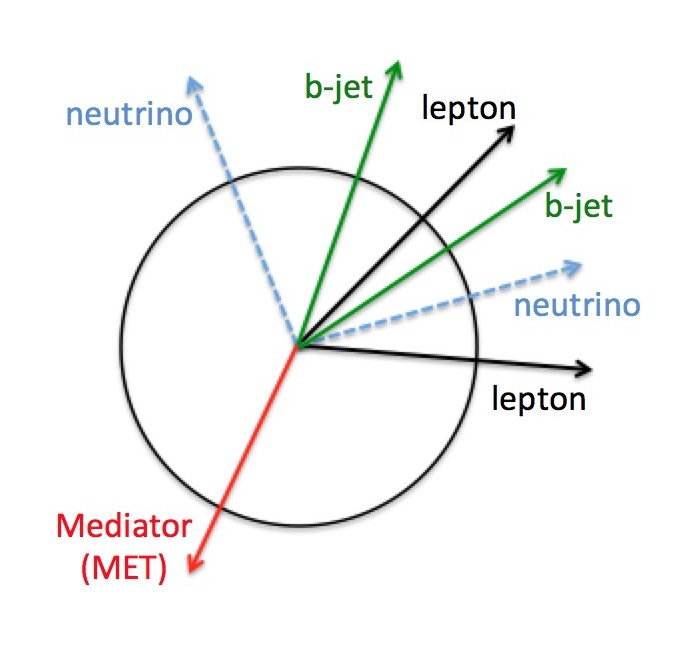
\includegraphics[width= 100pt, height= 100pt]{figs/deltaphi_high_mine.jpg} \\
	}
   \end{minipage} \hfill \vfill
   
   \begin{block}{}
   \vspace{5pt}
   \justifying
   We expect that the tops will be much closer to each other when the mass of the mediator produces raises, so this variable is expected to give some separation between the $t \bar t$ and the signal we are looking for, at least for high mediator masses. \vspace{5pt}
   \end{block} \vfill

\end{frame}


\begin{frame}{$m_{T2}^{ll}$ variable definition}

   	\justifying
	The variable $m_{T2}^{ll}$ has been introduced to measure the mass of a pair of particle produced in the particular case where both these particles decay into a final state including an undetected particle (neutrinos in this case). \\ \vspace{8pt}
	The problem is that in this case we can only know the total amount of $E_T^{\text{miss}}$ of the event considered and there is no way to know the exact contribution to this value given by each neutrino separately. We then need to calculate the transverse mass for the two pairs of particles, for different repartitions of $E_T^{\text{miss}}$. The repartition giving rise to the smallest possible mass is kept as the value of $m_{T2}^{ll}$. \\ \vspace{8pt}
	
\begin{equation*}
	\begin{cases}
	\vspace{8pt}
	\left(M_T^{(i)}\right)^2 = \left(m_{vis}^{(i)}\right)^2 + m_{\chi}^2 + 2 \cdot \left(E_{T}^{vis(i)} E_{T}^{\chi(i)} - \overrightarrow{p}_{T}^{vis(i)} \cdot \overrightarrow{p}_{T}^{\chi(i)}\right) \\ 
m_{T2}\left(m_\chi \right) = \min_{\sum_{i}{\overrightarrow{p}_{T}^{\chi(i)}}}\left[{\max{\left(M_T^{(1)}, M_T^{(2)}\right)}}\right]
	\end{cases}
\end{equation*}
	
	\begin{block}{}
	\vspace{5pt}
	\justifying
	We expect this variable to give some discrimination between $t \bar t$ and our signal because we know that the transverse mass obtained this way for the W has to take values less or equal than the actual mass of the W. However, the presence of additional $E_T^{\text{miss}}$ coming for the dark matter can break this condition. \vspace{5pt}
	\end{block} \vfill

\end{frame}


\begin{frame}{$t \bar t$ control region}

	\justifying
	A \textbf{control region} is usually defined by several cuts in order to check for the validity of a process simulated by Monte Carlo. The control region then has to be defined in such a way that this region is \textbf{enriched in the process we are interested in}. \vfill
	
	This is why we created a control region for the $t \bar t$, our most important background. This region has been defined by removing the $E_T^{\text{miss}}$ and by reversing the cut in $m_{T2}^{ll}$. As always, the 10 GeV signal is represented with the red line and has been rescaled by a factor 10. \vfill

	\hspace{30pt}
   \begin{minipage}[c]{.42\linewidth}
   	\justifying
   	 The main objective of this control region is to calculate a \textbf{scale factor}, a factor by which we need to scale the considered process to get a perfect agreement between data and Monte Carlo.
	 \begin{block}{}
	 \justifying
	 In this case, we obtain a scale factor for the $t \bar t$ of $0.97 \pm 0.01$, the error being statistical only.
	 \end{block}
   \end{minipage} \hfill
    \begin{minipage}[c]{.48\linewidth}
	\begin{center}
	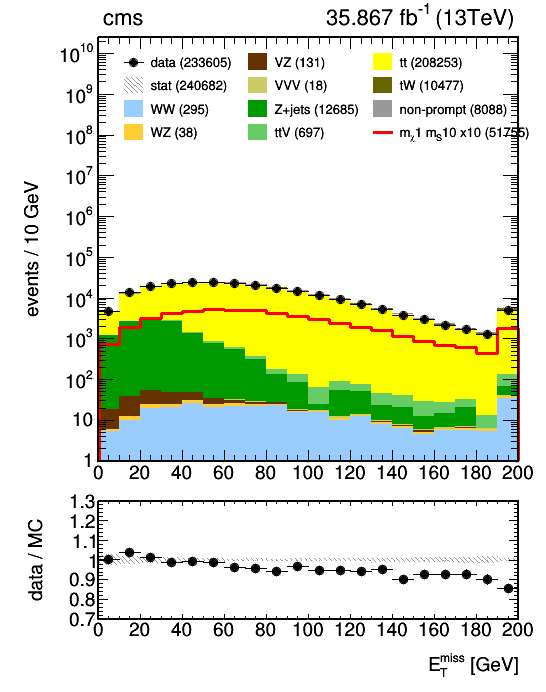
\includegraphics[width= 130pt, height= 130pt]{figs/metPfType1_log-ttCR2.png}
	\end{center}
   \end{minipage} \hfill \vfill

\end{frame}


\begin{frame}{Rin-out method}

	\justifying
	To estimate the Drell-Yan (DY), we calculated its importance using a data-driven method. This method consists basically in estimating the number of DY outside of the peak of the Z directly from the number of data events inside of the peak. \vfill

	\begin{center}
		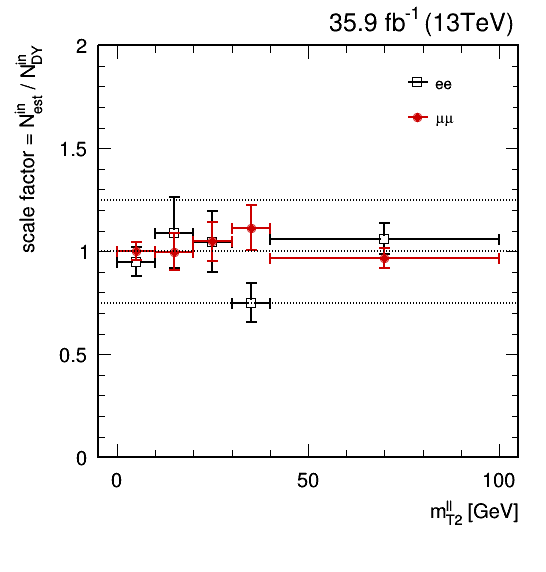
\includegraphics[width= 140pt, height= 140pt]{figs/dy_scale-4.png} \\
	\end{center}
	
	The scale factor obtained (1.07 $\pm$ 0.07) with this method has been applied to the usual MC simulations for the Drell-Yan process. \vfill

\end{frame}


\begin{frame}{Fake rate}

	\justifying
	The fake rate corresponds to the probability to see a fake lepton (usually misidentified from a jet) passing the cuts corresponding to the final selection level of the analysis. This rate is estimated for both electrons and muons, within a QCD-enriched control region, by removing the contamination coming from the Z+jets and W+jets processes. \vfill

\hspace{4pt}
   \begin{minipage}[c]{.02\linewidth}
	\begin{exampleblock}{} \rotatebox{90}{ Electron FR } \end{exampleblock}
   \end{minipage}	
   \hspace{5pt}	
	\begin{minipage}[c]{.48\linewidth}
   	\centering{
		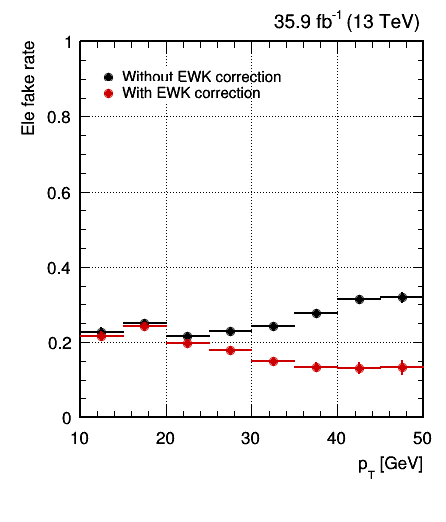
\includegraphics[width= 110pt, height= 95pt]{figs/Ele_FR_pt_35GeV.png}
	}
   \end{minipage} \hfill
   \begin{minipage}[c]{.48\linewidth}
   	\centering{
		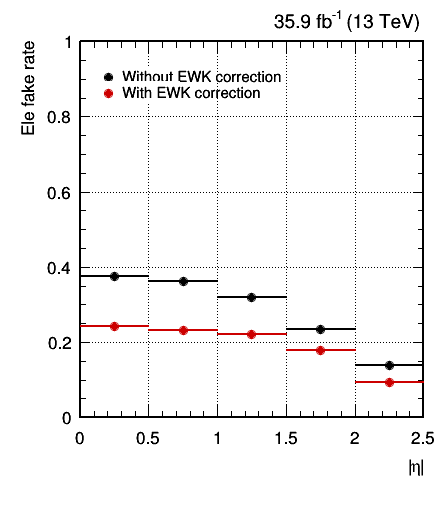
\includegraphics[width= 110pt, height= 95pt]{figs/Ele_FR_eta_35GeV.png} \\
	}
   \end{minipage} \hfill
   
   \vspace{-8pt}
   
   \hspace{4pt}
   \begin{minipage}[c]{.02\linewidth}
	\begin{exampleblock}{} \rotatebox{90}{ Muon FR } \end{exampleblock}
   \end{minipage}	
   \hspace{5pt}
  \begin{minipage}[c]{.48\linewidth}
   	\centering{
		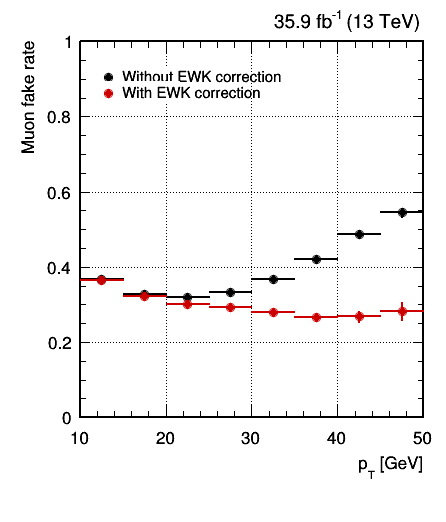
\includegraphics[width= 110pt, height= 95pt]{figs/Muon_FR_pt_25GeV.png}
	}
   \end{minipage} \hfill
   \begin{minipage}[c]{.48\linewidth}
   	\centering{
		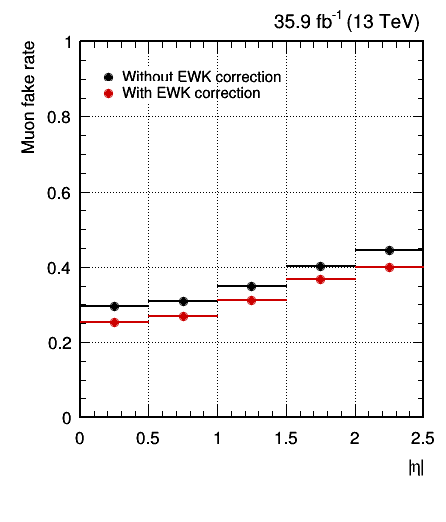
\includegraphics[width= 110pt, height= 95pt]{figs/Muon_FR_eta_25GeV.png} \\
	}
   \end{minipage} \hfill \vfill

\end{frame}


\begin{frame}{Prompt rate}

	\justifying
	The prompt rate is calculated thanks to a general tag and probe method and is useful to take into account the real lepton contamination in the control region we defined to calculate the fake rate. \vfill
	
	\hspace{4pt}
	\begin{minipage}[c]{.02\linewidth}
	\begin{exampleblock}{} \rotatebox{90}{ Electron PR } \end{exampleblock}
   \end{minipage}
	\begin{minipage}[c]{.48\linewidth}
   	\centering{
		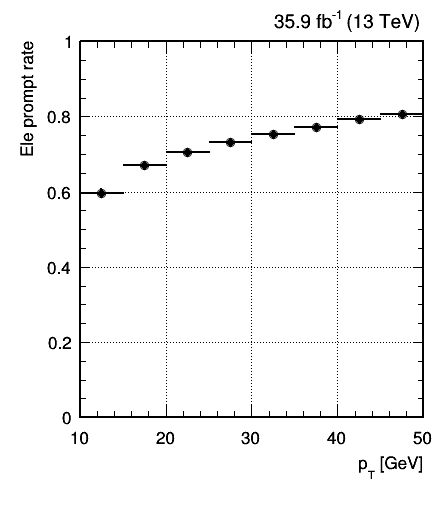
\includegraphics[width= 110pt, height= 95pt]{figs/Ele_PR_pt.png}
	}
   \end{minipage} \hfill
   \begin{minipage}[c]{.48\linewidth}
   	\centering{
		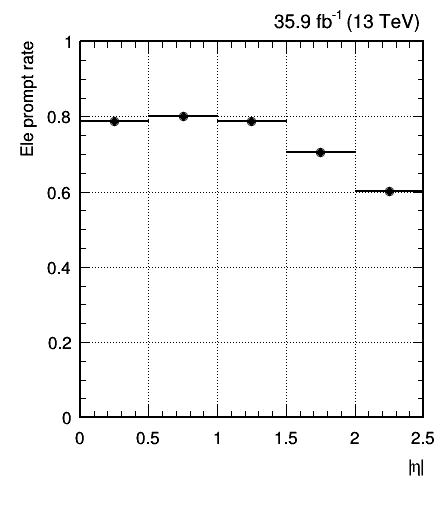
\includegraphics[width= 110pt, height= 95pt]{figs/Ele_PR_eta.png} \\
	}
   \end{minipage} \hfill
   
   \hspace{4pt}
   \begin{minipage}[c]{.02\linewidth}
	\begin{exampleblock}{} \rotatebox{90}{ Muon PR } \end{exampleblock}
   \end{minipage}
   \begin{minipage}[c]{.48\linewidth}
   	\centering{
		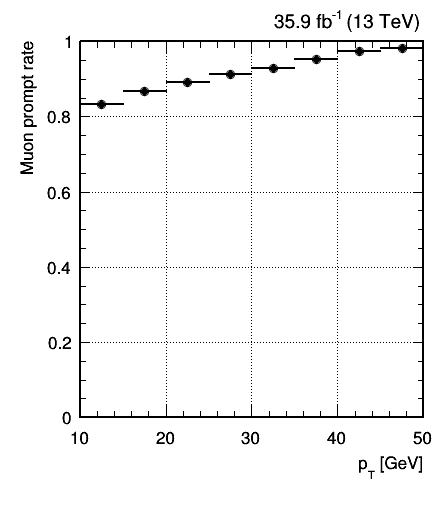
\includegraphics[width= 110pt, height= 95pt]{figs/Muon_PR_pt.png}
	}
   \end{minipage} \hfill
   \begin{minipage}[c]{.48\linewidth}
   	\centering{
		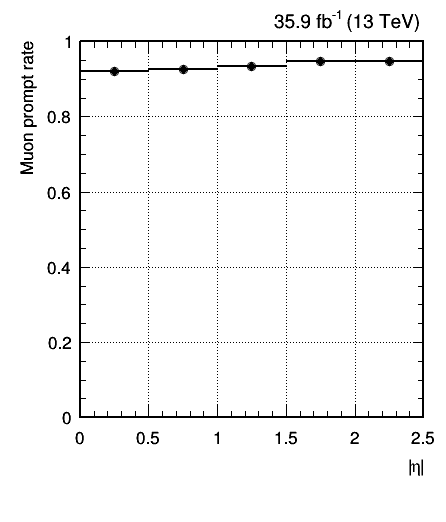
\includegraphics[width= 110pt, height= 95pt]{figs/Muon_PR_eta.png} \\
	}
   \end{minipage} \hfill \vfill

\end{frame}


\begin{frame}{Overtraining issue of the ANN}

	\justifying
	We can check for eventual signs of overtraining for the different neural networks built. This can be done thanks to the convergence plots. \vfill
	
   \hspace{4pt}
   \begin{minipage}[c]{.02\linewidth}
	\begin{exampleblock}{} \rotatebox{90}{ $m_\Phi$ = 10 GeV} \end{exampleblock}
   \end{minipage}	
   \hspace{5pt}	
   \begin{minipage}[c]{.44\linewidth}
   	\centering{
	\begin{exampleblock}{}{ \begin{center}  Activation function 1 \end{center}} \end{exampleblock} \vspace{5pt}
		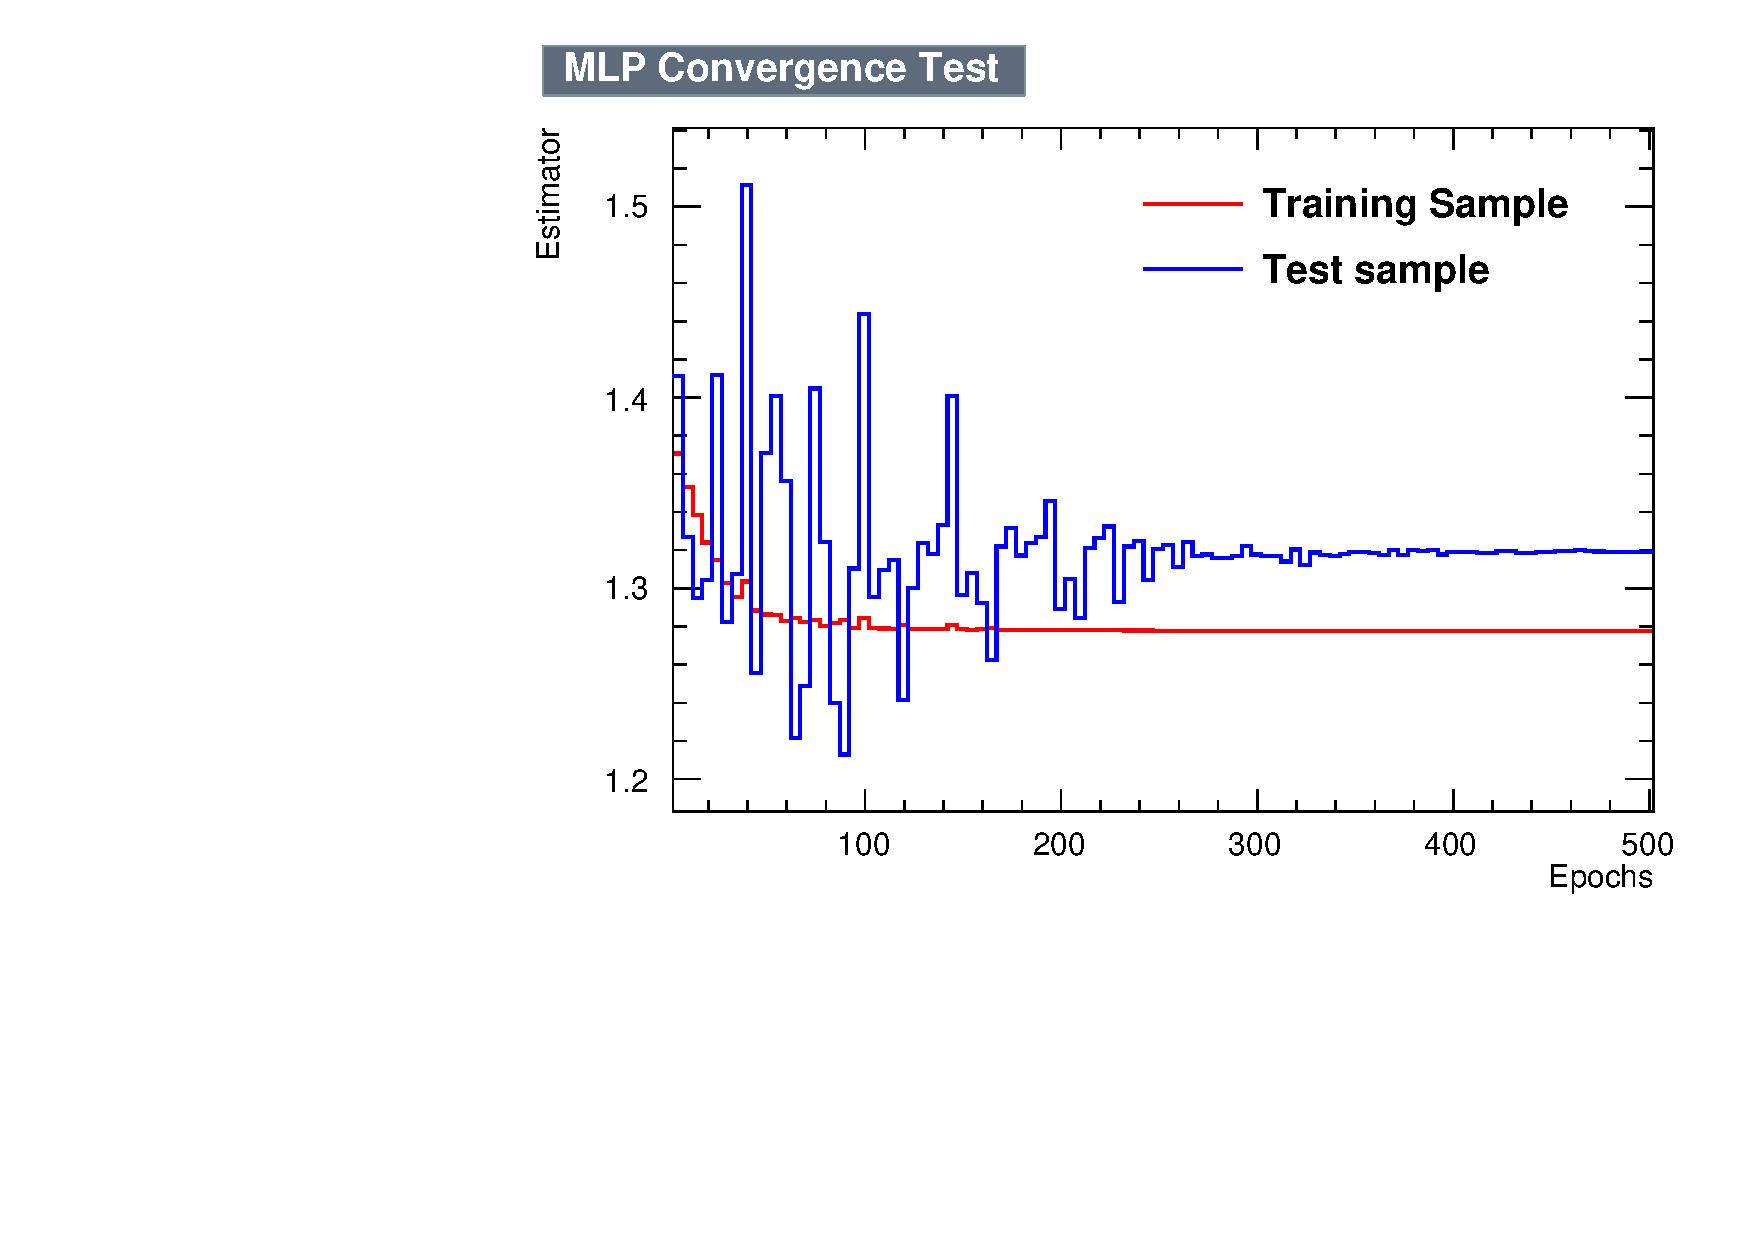
\includegraphics[width= 110pt, height= 87pt]{figs/newMVA/convergence_sigmoid_10GeV.pdf}
	}
   \end{minipage} \hfill
   \begin{minipage}[c]{.44\linewidth}
   	\centering{
		\begin{exampleblock}{}{ \begin{center} Activation function 2 \end{center}} \end{exampleblock} \vspace{5pt}
		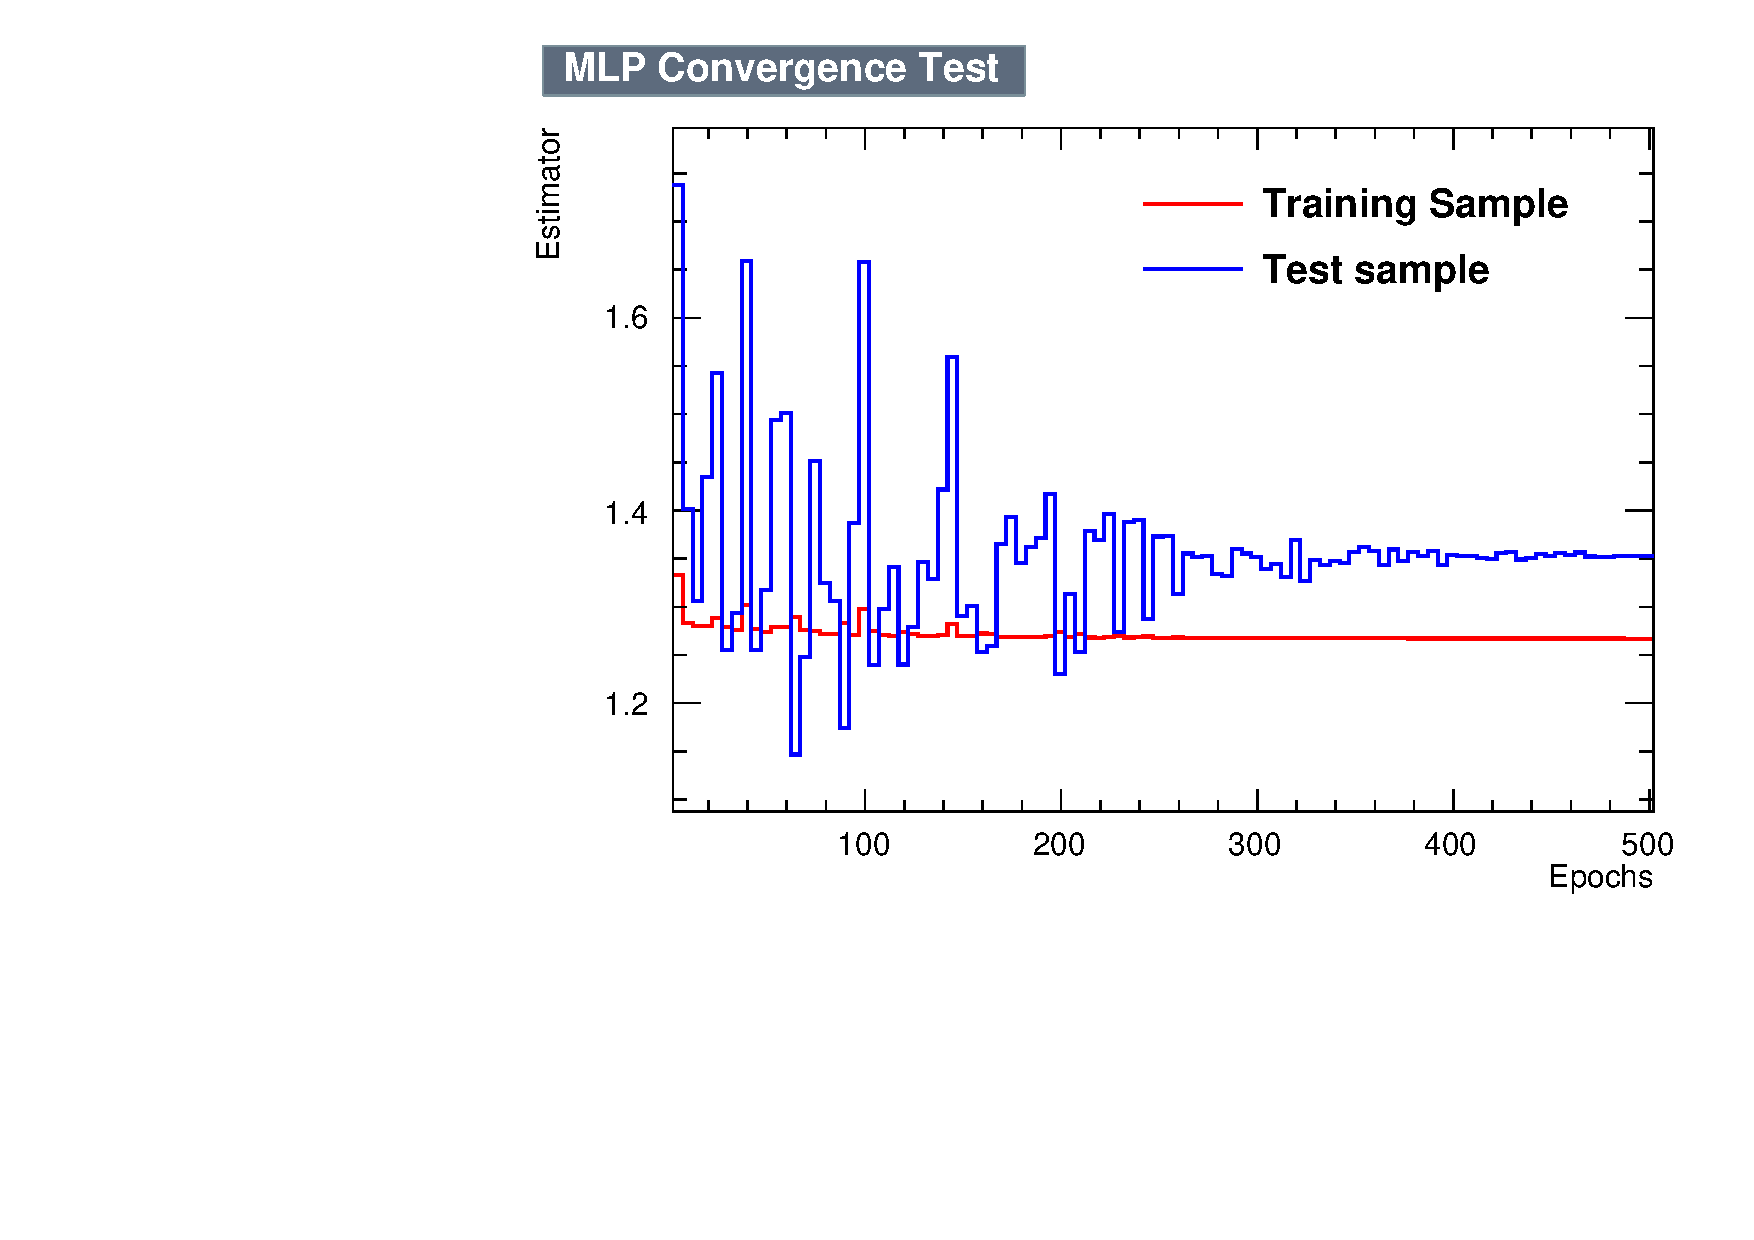
\includegraphics[width= 110pt, height= 87pt]{figs/newMVA/convergence_tanh_10GeV.pdf}
	}
   \end{minipage} \hfill
   
   \hspace{4pt}
    \begin{minipage}[c]{.02\linewidth}
	\begin{exampleblock}{} \rotatebox{90}{ $m_\Phi$ = 500 GeV} \end{exampleblock}
   \end{minipage}	
   \hspace{5pt}
   \begin{minipage}[c]{.44\linewidth}
   	\centering{
		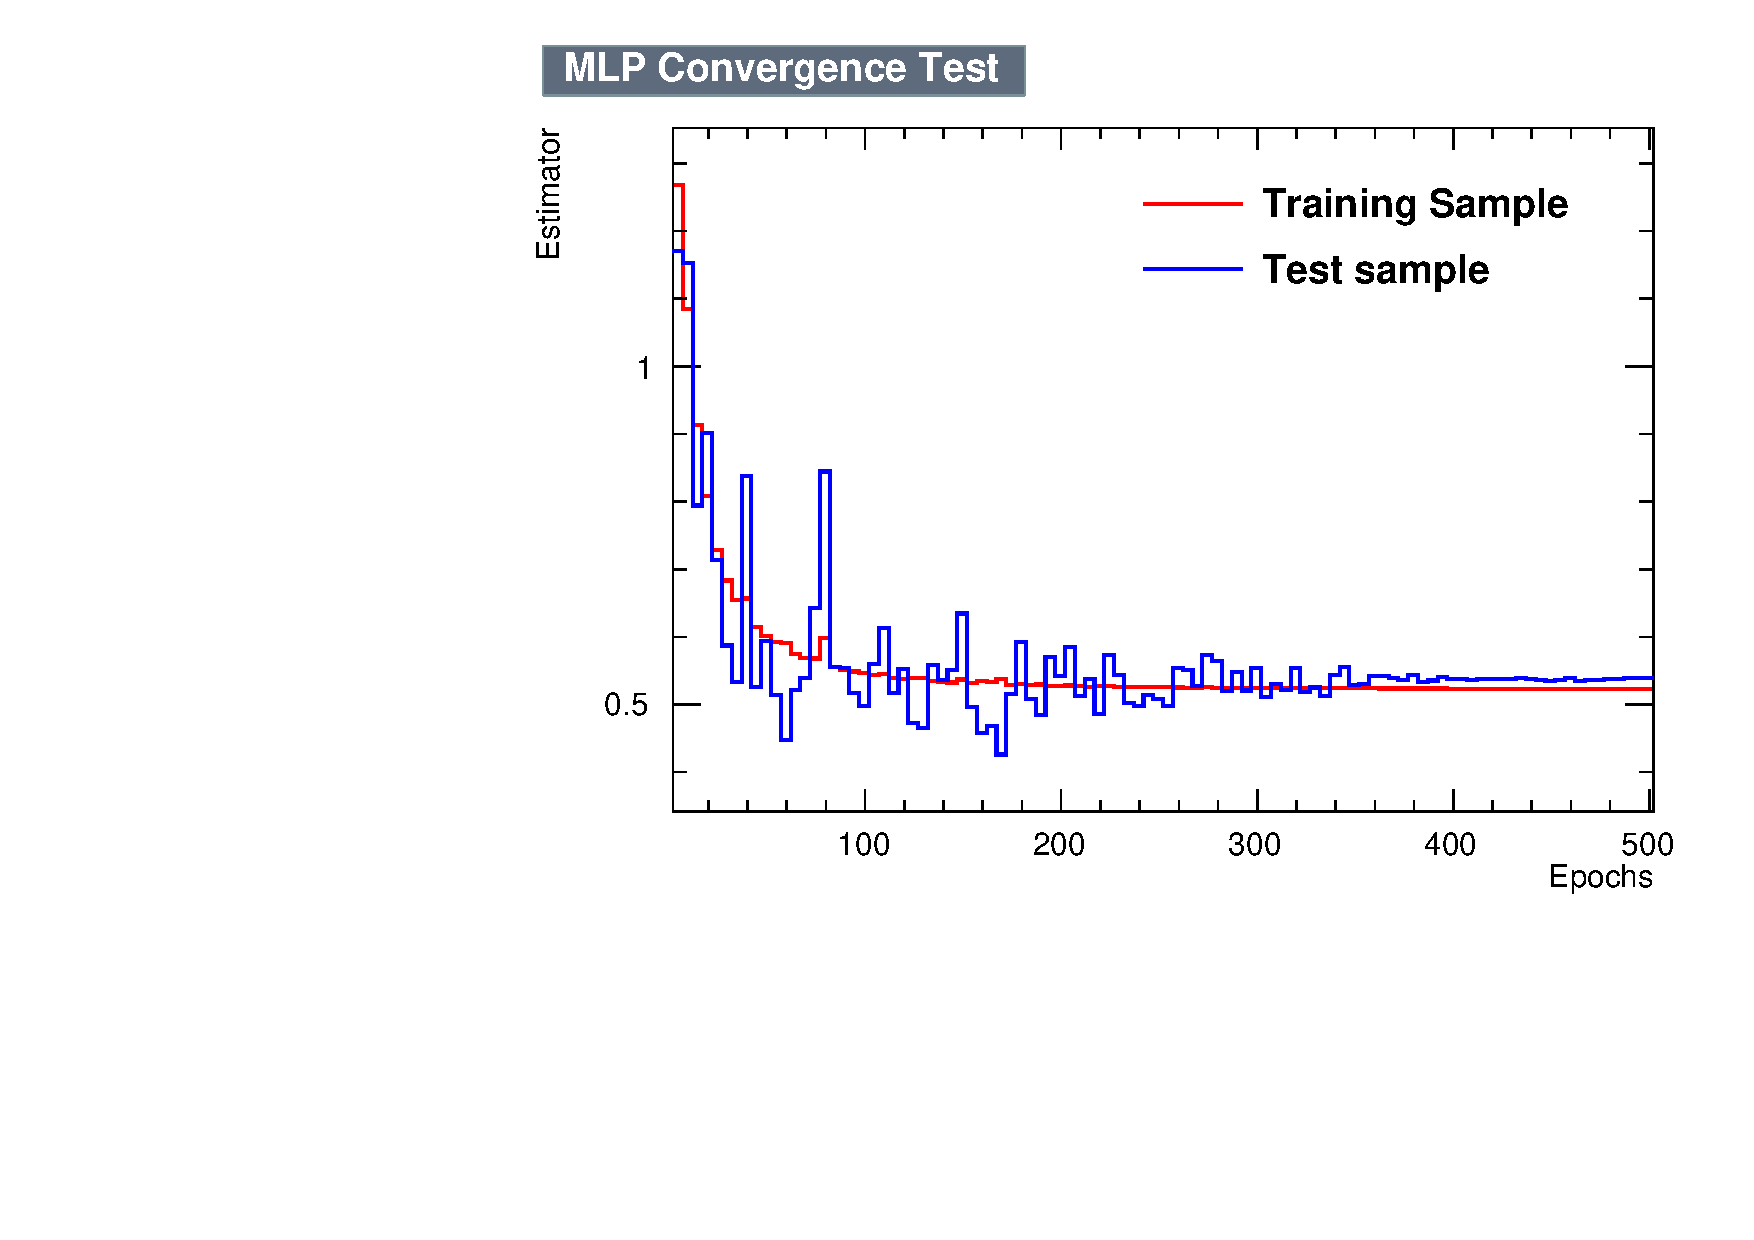
\includegraphics[width= 110pt, height= 87pt]{figs/newMVA/convergence_sigmoid_500GeV.pdf}
	}
   \end{minipage} \hfill
   \begin{minipage}[c]{.44\linewidth}
   	\centering{
		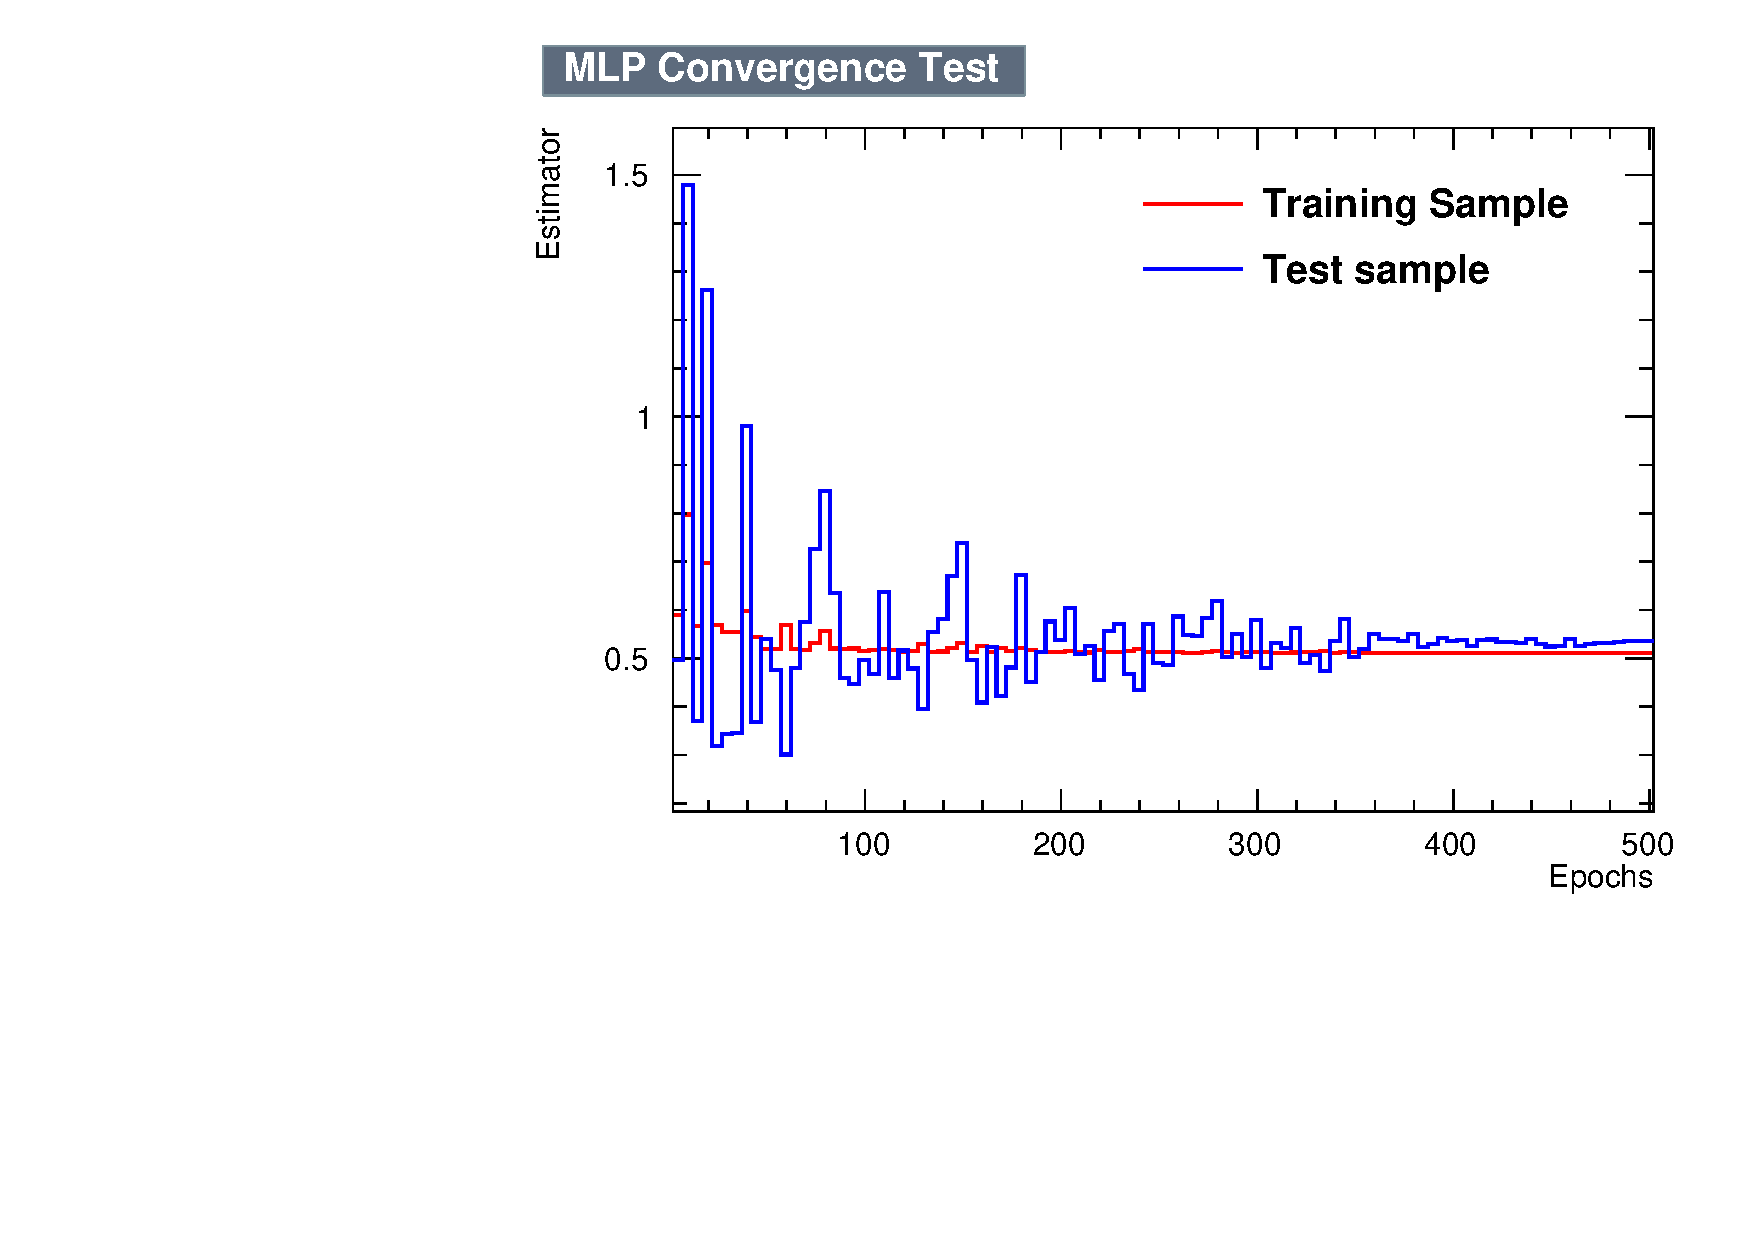
\includegraphics[width= 110pt, height= 87pt]{figs/newMVA/convergence_tanh_500GeV.pdf}
	}
   \end{minipage} \hfill \vfill

\end{frame}


\begin{frame}{ROC curves of the ANN}

	\justifying
 The ROC curves represent the signal efficiency possible to achieve with the neural network considered, given any background rejection we are interested in. Here are compared the ROC curves obtained for both the sigmoid and tanh activation functions, and for both the 10 and 500 GeV networks. As we can see, we can achieve a much better background rejection for any given signal efficiency in the 500 GeV case. \vfill

   \begin{minipage}[c]{.48\linewidth}
       \begin{exampleblock}{} { \begin{center} 10 GeV network \end{center}} \end{exampleblock} \vspace{10pt}
   	\centering{
		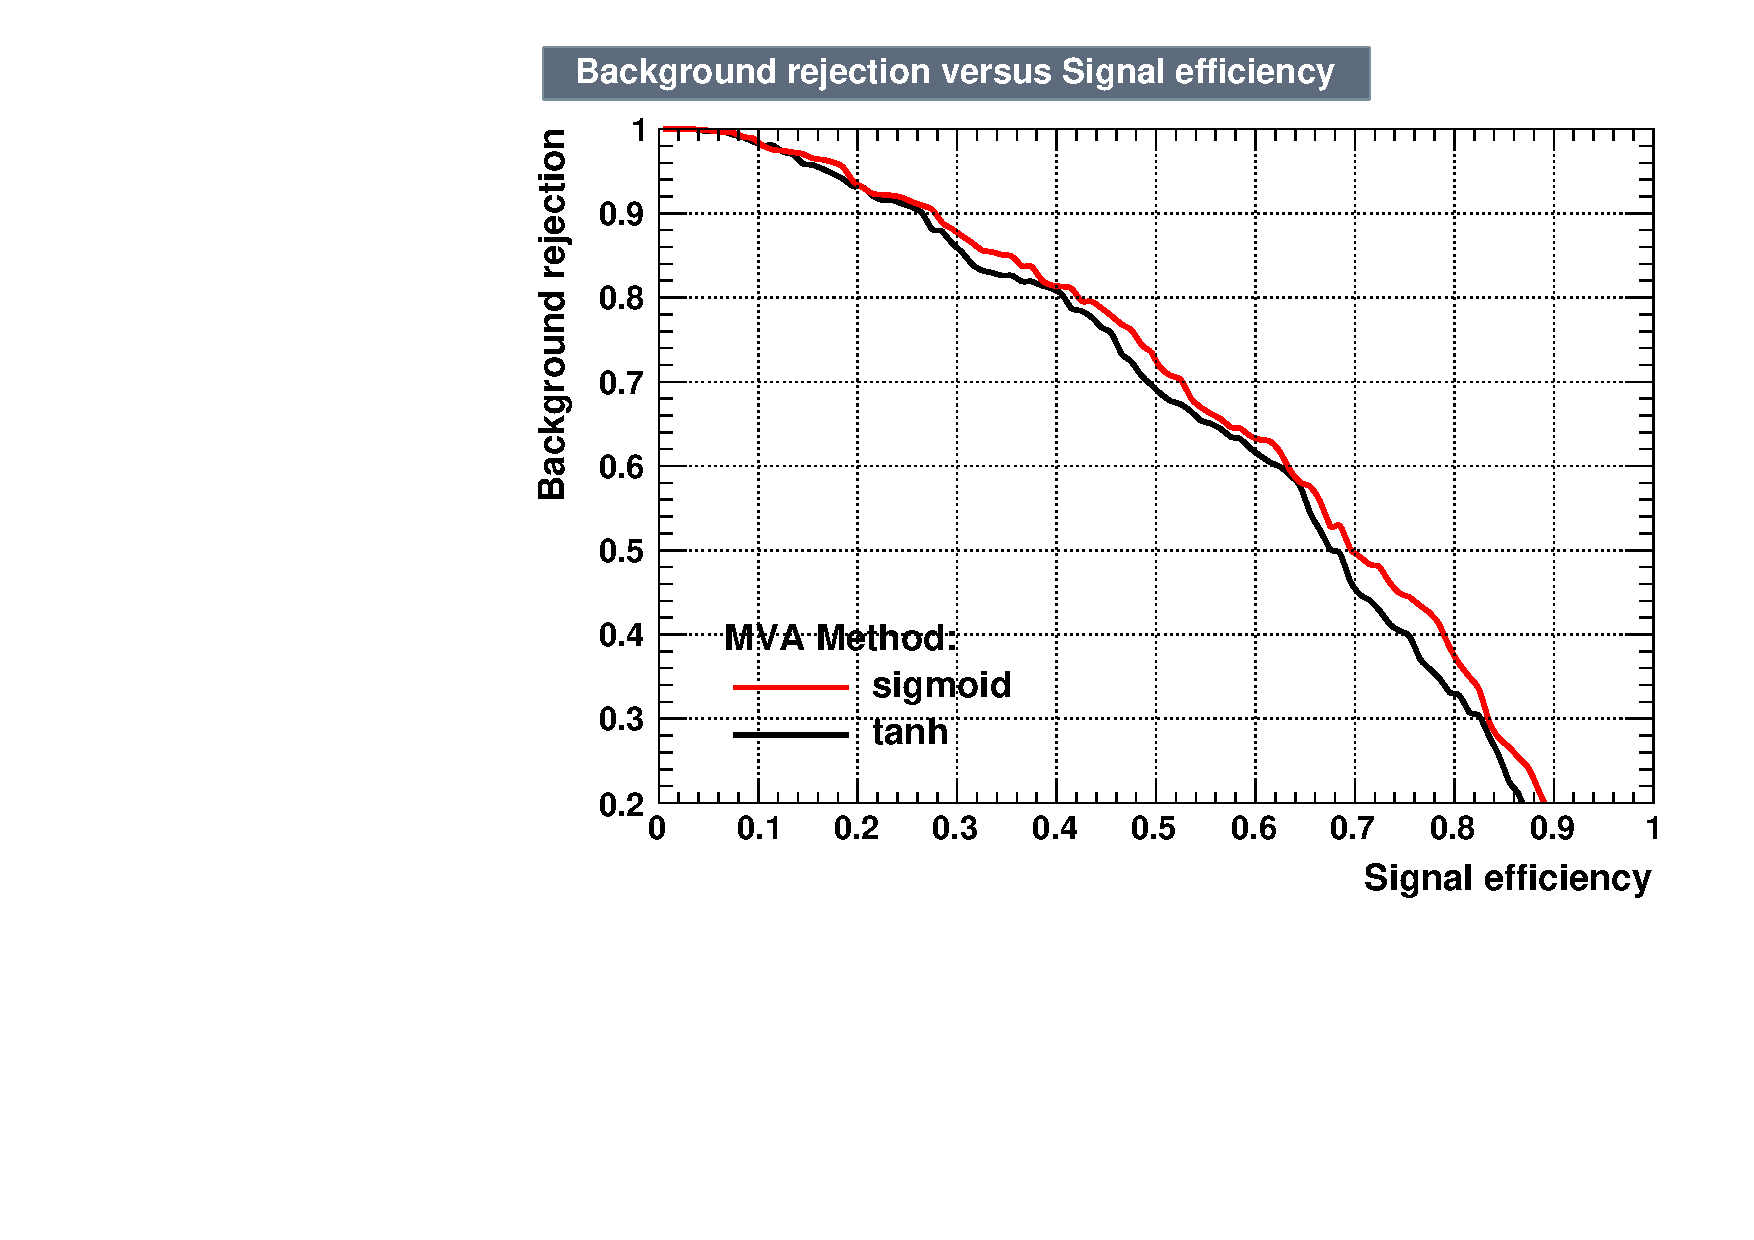
\includegraphics[width= 140pt, height= 120pt]{figs/newMVA/ROC_10GeV.pdf}
	}
   \end{minipage} \hfill
   \hspace{4pt}
   \begin{minipage}[c]{.48\linewidth}
   	\begin{exampleblock}{} {\begin{center} 500 GeV network \end{center}} \end{exampleblock} \vspace{10pt}
   	\centering{
		\includegraphics[width= 140pt, height= 120pt]{figs/newMVA/ROC_500GeV.pdf}
	}
   \end{minipage} \hfill \vfill
	
\end{frame}


\begin{frame}{Output of the ANN}

\justifying
We can also study the output of the different neural networks, and its significance curve which are helpful to find the optimal cut to apply to the analysis, to get the best significance possible. \vfill

   \begin{minipage}[c]{.48\linewidth}
       \begin{exampleblock}{} { \begin{center} 10 GeV network \end{center}} \end{exampleblock} \vspace{2pt}
   	\centering{
		\includegraphics[width= 95pt, height= 82pt]{figs/ANN_sigm_mt2ll80_Cedrictest_ttDM0001scalar00010_significance.png} \\
		\includegraphics[width= 100pt, height= 90pt]{figs/ANN_sigm_mt2ll80_Cedrictest_ttDM0001scalar00010_log.png}
	}
   \end{minipage} \hfill
   \hspace{4pt}
   \begin{minipage}[c]{.48\linewidth}
   	\begin{exampleblock}{} {\begin{center} 500 GeV network \end{center}} \end{exampleblock} \vspace{2pt}
   	\centering{
		\includegraphics[width= 95pt, height= 82pt]{figs/ANN_sigm_mt2ll80_Cedrictest_ttDM0001scalar00500_significance.png} \\
		\includegraphics[width= 100pt, height= 90pt]{figs/ANN_sigm_mt2ll80_Cedrictest_ttDM0001scalar00500_log.png}

	}
   \end{minipage} \hfill \vfill

\end{frame}


\begin{frame}{Yields table (pseudoscalar mediator)}

	\justifying 
	We can now represent the yields obtained for the different backgrounds with the associated systematics, for the different background processes and different dark matter mediator mass points (and therefore, different neural networks). \vfill
	
	\begin{minipage}[c]{.48\linewidth}
	
	\begin{center}
	
	\begin{exampleblock}{}{ \begin{center} 10 GeV pseudo (ANN output $>$ 0.80) \end{center}} \end{exampleblock} \vspace{8pt}
	
	\resizebox{170pt} {!}{
	\begin{tabular}{c|c|c|c}
	 	& & & \\
		Process & Yields & Statistical error & Systematic error \\
		& & & \\
		\hline \hline
		& & & \\
		$t \bar t$ & 8.28 & 0.15 & 0.42 \\
		Non-prompt & 0.30 & 0.65 & 0.10 \\
		ttV & 0.74 & 0.03 & 0.18 \\
		Single top & 0.35 & 0.06 & 0.01 \\
		Drell-Yan & 0.39 & 0.28 & 0.12 \\
		WW & 0.02 & 0.02 & 0.01 \\
		& & & \\
		\hline
		& & & \\
		Total background & 10.08 & 0.72 & 0.48 \\
		& & & \\
		\hline
		& & & \\
		Signal & 0.89 & 0.02 & 0.45 \\
		Total with signal & 10.97 & 0.73 & 0.66 \\
		& & & \\
		\hline
		& & & \\
		Data & 8 & - & - \\
		& & & \\
	\end{tabular}
	} 
	
	\end{center}

	\end{minipage} \hfill
	\begin{minipage}[c]{.48\linewidth}
	
	\begin{exampleblock}{}{ \begin{center} 500 GeV pseudo (ANN output $>$ 0.98) \end{center}} \end{exampleblock} \vspace{8pt}
	
	\resizebox{170pt} {!}{
	\begin{tabular}{c|c|c|c}
	 	& & & \\
		Process & Yields & Statistical error & Systematic error \\
		& & & \\
		\hline \hline
		& & & \\
		$t \bar t$ & 0.81 & 0.05 & 0.04 \\
		Non-prompt & 0.10 & 0.31 & 0.03 \\
		ttV & 0.46 & 0.02 & 0.12 \\
		Single top & 0.04 & 0.02 & 0.01 \\
		Drell-Yan & 0.00 & 0.00 & 0.00 \\
		WW & 0.01 & 0.01 & 0.01 \\
		& & & \\
		\hline
		& & & \\
		Total background & 1.42 & 0.32  & 0.13 \\
		& & & \\
		\hline
		& & & \\
		Signal & 0.03 & 0.01 & 0.01 \\
		Total with signal & 1.45 & 0.32 & 0.13 \\
		& & & \\
		\hline
		& & & \\
		Data & 1 & - & - \\
		& & & \\
	\end{tabular}
	} 
	
	\end{minipage} \hfill \vfill

\end{frame}


\begin{frame}{Complete 2016 dataset expected limits}

	\justifying
	From the 2.4 fb$^{-1}$ limits we calculated, it is actually easy to estimate the expected limits when considering the complete 35.9 fb$^{-1}$ dataset, since we know that the limits are expected to decrease as the square root of the increase in luminosity. An increase of a factor 15 in the luminosity should then result in limits 4 times smaller. \vfill

   \begin{center}
   	 \begin{minipage}[c]{.48\linewidth}
	 \begin{exampleblock}{} { \begin{center} Scalar mediator \end{center}} \end{exampleblock}
    	\begin{center}
   	\begin{tabular}{c|c}
		& \\
		$m_S$ [GeV]& Expected limit  \\ 
		& \\ 
		\hline \hline
		& \\
		10 &  0.77\\
            	20 &  0.81\\
            	50 & 1.07 \\
            	100 & 1.82  \\
            	200 & 6.55 \\
            	300 & 14.00\\
            	500 & 45.31 \\
		& \\
          \end{tabular}
          \end{center}
   \end{minipage} \hfill
   \begin{minipage}[c]{.48\linewidth}
   	\begin{exampleblock}{} { \begin{center} Pseudoscalar mediator \end{center}} \end{exampleblock}
   	\begin{center}
   	\begin{tabular}{c|c}
		& \\
		$m_P$ [GeV]& Expected limit  \\ 
		& \\ 
		\hline \hline
		& \\
		10 & 2.44 \\
            	20 & 2.57  \\
            	50 & 2.96  \\
            	100 & 2.84 \\
            	200 & 4.47 \\
            	300 & 8.55 \\
            	500 & 43.36 \\
		& \\
          \end{tabular}
          \end{center}
   \end{minipage} \hfill \vfill
   \end{center}
   
   By considering the complete 2016 dataset, we therefore expect to be able to exclude with our analysis the 10 and 20 GeV scalar mediators. \vfill

\end{frame}


%\begin{frame}{Additional references}

%[1] ...

%\end{frame}

\backupend


 \end{document}